\documentclass[11pt,a4paper]{article}

\usepackage[T1]{fontenc}
\usepackage[utf8]{inputenc}
\usepackage{mathpazo}
\usepackage{amsmath,amssymb,amsthm}
\usepackage[margin=2.6cm]{geometry}
\usepackage{tikz}
\usepackage{booktabs}
\usepackage{enumitem}
\usepackage{multicol}
\usepackage{microtype}
\usepackage[hidelinks]{hyperref}
\hypersetup{
  pdftitle={Three-Piece Siege on the 4x4 Board is a Draw},
  pdfauthor={Anonymous},
  pdfsubject={Computer-assisted non-loss proof via safety certificates},
  pdfkeywords={combinatorial game theory, certifying algorithms, safety games, retrograde analysis}
}

\theoremstyle{plain}
\newtheorem{theorem}{Theorem}[section]
\newtheorem{lemma}[theorem]{Lemma}
\newtheorem{proposition}[theorem]{Proposition}
\newtheorem{corollary}[theorem]{Corollary}
\theoremstyle{definition}
\newtheorem{definition}[theorem]{Definition}
\newtheorem{remark}[theorem]{Remark}
\newtheorem{example}[theorem]{Example}

\newcommand{\bl}{\mathsf{b}}
\newcommand{\wh}{\mathsf{w}}
\newcommand{\St}{\mathcal{S}}
\newcommand{\Act}{\mathcal{A}}
\newcommand{\Mv}{\mathcal{M}}
\newcommand{\Zc}{\mathcal{Z}}
\newcommand{\Rg}{\mathcal{R}}
\newcommand{\wins}{\top}
\newcommand{\vv}[1]{\mathbf{#1}}
\newcommand{\sqn}[1]{\mathtt{#1}}

\newcommand{\Npos}{3{,}723{,}720}
\newcommand{\Nwin}{2{,}097{,}414}
\newcommand{\Nlose}{1{,}053{,}186}
\newcommand{\Ndraw}{573{,}120}
\newcommand{\Ncert}{91{,}330}
\newcommand{\NcertB}{63{,}885}
\newcommand{\NcertW}{27{,}445}
\newcommand{\NcertFF}{26{,}646}
\newcommand{\NcertFT}{28{,}800}
\newcommand{\NcertTF}{13{,}042}
\newcommand{\NcertTT}{22{,}842}
\newcommand{\Nshapes}{153}
\newcommand{\Nshapesfour}{83}
\newcommand{\Nshapesthree}{70}
\newcommand{\Nshapescanon}{79}
\newcommand{\Nregionshapes}{330}
\newcommand{\NlayerthreeW}{8{,}968}
\newcommand{\NlayerfourW}{18{,}477}
\newcommand{\Nlayerthreeb}{26{,}916}
\newcommand{\Nlayerfourb}{36{,}969}
\newcommand{\Nnocapthree}{8{,}968}
\newcommand{\Nbaitpos}{1{,}999}
\newcommand{\Nbaitbad}{0}
\newcommand{\Nbookshapes}{79}
\newcommand{\Nbookcand}{121}
\newcommand{\Nbookcond}{849}
\newcommand{\Nbookrules}{970}
\newcommand{\Nsigma}{30{,}245}
\newcommand{\NsigmaBdec}{21{,}267}
\newcommand{\NsigmaWnodes}{8{,}978}
\newcommand{\NsigmaBwin}{6{,}268}
\newcommand{\NsigmaBstuck}{0}
\newcommand{\Nomega}{25{,}274}
\newcommand{\NomegaWdec}{17{,}756}
\newcommand{\NomegaBnodes}{7{,}518}
\newcommand{\NomegaWwin}{5{,}912}
\newcommand{\NomegaWstuck}{0}
\newcommand{\Nsigmashapes}{151}
\newcommand{\Nsigmafour}{21{,}219}
\newcommand{\Nsigmathree}{9{,}026}
\newcommand{\Ndrawplies}{12}
\newcommand{\Nrepplies}{4, 8, 12}
\newcommand{\Ncanondrawgame}{1.B $42$--$32$ 2.W $14$--$24$ 3.B $43$--$42$ 4.W $12$--$22$ 5.B $44$--$43$ 6.W $11$--$12$ 7.B $43$--$44$ 8.W $12$--$11$ 9.B $44$--$43$ 10.W $11$--$12$ 11.B $43$--$44$ 12.W $12$--$11$}
\newcommand{\Nsharp}{8{,}974}
\newcommand{\Nsharppct}{42\%}
\newcommand{\Ngoodpct}{84\%}
\newcommand{\Nwcfgmin}{107}
\newcommand{\Nwcfgmax}{1{,}070}
\newcommand{\Nfortresswin}{489}
\newcommand{\Nfortressdraw}{6}
\newcommand{\Nfortresstotal}{495}
\newcommand{\Nfortresswwin}{0}
\newcommand{\Nfortresswlose}{455}
\newcommand{\Nfortresswdraw}{40}
\newcommand{\Nfourshapes}{1{,}820}

\newcommand{\Nfourshapesall}{1{,}820}
\newcommand{\Nfortressnum}{1}
\newcommand{\Nfortbwin}{489}
\newcommand{\Nfortblose}{0}
\newcommand{\Nfortbdraw}{6}
\newcommand{\Nfortwwin}{0}
\newcommand{\Nfortwlose}{455}
\newcommand{\Nfortwdraw}{40}
\newcommand{\Nfortbwinth}{220}
\newcommand{\Nfortbdrawth}{0}
\newcommand{\Nfortwloseth}{220}

\newcommand{\Nexentry}{29}
\newcommand{\Nexrules}{7}
\newcommand{\Nexcoords}{\sqn{31}, \sqn{32}, \sqn{42}, \sqn{43}}
\newcommand{\Nfortentry}{--}
\newcommand{\Nfortrules}{0}


\title{\bf Three-Piece Siege on the $4\times4$ Board is a Draw:\\
A Certificate-Based Proof via Safety Games and a Colour-Reversible Rule Book}
\author{Anonymous submission}
\date{22 August 2026}

\begin{document}
\maketitle

\begin{abstract}
\emph{Three-Piece Siege} is a $4\times4$ board game with single-step moves, mandatory
line captures, loss by reduction to two men or by immobility, and a draw by threefold
repetition of the full position. We prove that the game is a draw, and we do so without
appealing to a database of game values. The proof rests on one explicitly given object:
a set $S$ of $\Ncert$ positions together with two elementary properties --- $S$ is closed
in the sense of a \emph{safety game} for Black, and $S$ contains the initial position both
with Black and with White to move. The rules admit a colour-reversing automorphism $\rho$
(a $180^\circ$ rotation composed with the exchange of the two colours and of the side to
move) which carries the initial position with White to move to the initial position with
Black to move; hence $\rho(S)$ is a corresponding certificate for White, and neither player
has a winning strategy. Checking the certificate requires no fixed-point iteration, no
search and no table of values: it is a single pass of local tests over the $\Npos$
positions, and takes $0.12$ seconds.

From $S$ we extract a memoryless strategy $\Pi$ presented as $\Nbookshapes$
shape-indexed ordered decision lists over atomic predicates on the opponent's men
($\Nbookrules$ rules in total). Black plays $\Pi$ and White plays its conjugate
$\Pi^\rho$; exhaustive expansions of the opponent's moves give reachable sets of
$\Nsigma$ and $\Nomega$ positions. The Black-strategy reachable set $\Sigma$, which is
$67\%$ smaller than $S$, is itself a valid certificate, so the whole proof can be carried
by an object one player can actually execute by hand. When both sides follow their
respective conjugate books, the game is drawn after $\Ndrawplies$ plies. An auxiliary
history-free retrograde classification of all $\Npos$ positions serves only as
corroboration: it identifies the central $2\times2$ block as the unique four-man shape
that is safe against \emph{every} opposing configuration. This is a local structural
fact; it makes no claim about forcing that shape from the initial position.

We stress the precise scope of this claim. What is proved, rigorously and independently
of any table of values, is that under the rules' history-dependent threefold-repetition
clause each player has a \emph{positional} (memoryless, history-blind) strategy that
guarantees at least a draw. Lemma~\ref{lem:finite} guarantees termination; it is
Theorem~\ref{thm:sound}, not finiteness alone, that establishes the effectiveness of the
constructed position-only safety strategies. The verification is
computer-assisted rather than machine-formalised: the published C verifier and Python
rule-book checker check the stated certificates (Section~\ref{sec:verify}), and no
proof-assistant formalisation (Coq, Lean, Isabelle) has been attempted. Nor is the
substance of the paper the size of the state space, which at $\Npos$ positions is small by
the standards of solved games; the substance is that the draw is certified without ever
constructing or trusting a value table, a distinction familiar from the theory of
certifying algorithms and one that scales to games whose value table is out of reach.
\end{abstract}

\section{Introduction}

Solving a finite two-player game of perfect information is, in principle, a triviality:
Zermelo's argument \cite{zermelo} assigns a value to every position by backward induction,
and retrograde analysis \cite{strohlein,romein} turns the argument into an algorithm.
In practice the difficulty is not obtaining the value but obtaining a \emph{proof} that a
reader can check. When the answer is produced by sweeping a table of $10^{6}$ or $10^{20}$
entries to a fixed point, the reader is asked to trust an iteration whose intermediate
states have no independent meaning. This is the difference, familiar from the theory of
certifying algorithms \cite{certifying}, between an algorithm that outputs an answer and
one that outputs a \emph{witness}.

For games whose value is a draw there is a particularly clean form of witness. To show
that a player $P$ cannot lose it suffices to exhibit a set of positions that is closed
under the opponent's moves, that $P$ can never be forced to leave, and in which $P$ is
never mated; the required properties are \emph{local} --- each is a statement about one
position and its immediate successors. Such sets are exactly the invariants of a
\emph{safety game}, and they are the greatest fixed points of a monotone operator
\cite{tarski,gtw}. A safety invariant is to a drawing strategy what a pairing strategy is
to a Hex or Y non-losing argument, or what a fortress is to an endgame evaluation: a
finite, checkable, human-inspectable object.

This paper carries out that programme for \emph{Three-Piece Siege}, a $4\times4$ board
game. The formal rule set used throughout (version 2.0, dated 22 August 2026 and reproduced
in full, section by section, in Section~\ref{sec:game}) was designed as a precise,
checkable, compact but nontrivial test case for the certificate method of
Section~\ref{sec:safety}. We make no claim to have discovered a previously
unknown game: the contribution of this paper is the proof method and its worked
instantiation, not the game itself. The rules (Section~\ref{sec:game}) are unusual in
three respects
that make the game genuinely difficult to analyse by hand: captures are \emph{mandatory}
and are triggered by the geometry of the destination square's row and column, so a player
can be forced to capture into a fork; a player who is reduced to two men loses at once,
so material is a cliff rather than a slope; and the draw rule is threefold repetition of
the full position \emph{including the side to move}, which makes the terminating condition
depend on the history rather than on the position.

Our results are the following.

\begin{itemize}[itemsep=2pt,topsep=3pt]
\item The game is a draw (Theorem~\ref{thm:main}). The proof needs a single explicitly
given set $S$ of $\Ncert$ positions, two local closure properties of $S$, and one
symmetry of the rules. It does not use the values of any position.
\item The history-dependence of the draw rule is harmless
(Lemma~\ref{lem:finite}): because each full position can occur at most three times, every
play has at most $2N+1$ moves with $N=\Npos$, so the game tree is finite. The
position-only non-loss claims are justified separately by the safety-certificate theorem
(Theorem~\ref{thm:sound}). This settles a caveat raised in the rules document itself.
\item There is a memoryless rule book $\Pi$ of $\Nbookrules$ rules, indexed by the
$\Nbookshapes$ shapes that Black's men may form. Black plays $\Pi$ directly, while White
plays the conjugate book $\Pi^\rho$ under the colour-reversing symmetry
(Theorem~\ref{thm:book}). The reachable set for $\Pi$, of only $\Nsigma$ positions, is
again a valid certificate (Theorem~\ref{thm:sigma}), so the strategy and the proof are
the same object.
\item The certificate has a transparent structure
(Propositions~\ref{prop:region}--\ref{prop:exchange}): all of Black's shapes live in a
fixed $10$-square region; Black concedes at most one man in the whole game; and once
Black is down to three men, White never again has a capturing move at all --- in none of
the $\NlayerthreeW$ relevant positions.
\item An auxiliary history-free retrograde classification (Section~\ref{sec:table}) is
used only as corroboration, not as an exact solution of the history-sensitive game. It
yields the local structural fact (Proposition~\ref{prop:fortress}) that, of the
$\Nfourshapesall$ four-man shapes, exactly $\Nfortressnum$ --- the central $2\times2$
block --- is safe against every opposing configuration.
\end{itemize}

Games have of course been solved by computer since the 1970s, and several are draws:
Connect Four is a first-player win \cite{allisthesis,allisconnect}, Nine Men's Morris is a
draw \cite{gasser}, Awari is a draw \cite{romein}, Fanorona is a draw \cite{fanorona}, and
Checkers is a draw \cite{checkers}. Reported state-space sizes for these games range from
the order of $10^{11}$--$10^{12}$ positions (Awari, Connect Four) to about $5\times10^{20}$
for Checkers \cite{checkers}; ours, at $\Npos$, is smaller by many orders of magnitude,
and that is deliberate --- a
small state space is what makes it feasible to also carry out, side by side, an auxiliary
history-free retrograde classification (Section~\ref{sec:table}) and a from-scratch, human-checkable
certificate (Sections~\ref{sec:safety}--\ref{sec:book}), so that the two can be compared.
In every one of the cited results the published witness is, in the end, a value database
plus the program that produced it: reproducing the proof means re-running that program (or
trusting its authors), because the database's intermediate states, being the output of a
fixed-point iteration, carry no independent meaning. This is exactly the distinction
between an algorithm and a \emph{certifying} algorithm \cite{certifying}: the latter emits,
together with its answer, a witness that a third party can check in time independent of
how the answer was found. Safety games \cite{tarski,gtw} are the certifying-algorithm
formulation of ``does not lose'' for a two-player game, in the same sense that a
satisfying assignment certifies satisfiability or a flow certifies a min-cut bound; what
this paper adds to that standard idea is (a) a construction disciplined enough to produce
a certificate small enough to typeset in an appendix, and (b) the observation, via the
colour-reversing symmetry of Section~\ref{sec:sym}, that for a symmetric game a single such
certificate can be transferred to serve both players at once, halving the construction
work. What is new is therefore not the scale of the example but the \emph{form} of the
argument: the entire mathematical content is two closure conditions on one exhibited set,
verified by a $232$-line program that performs no search and consults no value table; the
same recipe applies unchanged to any two-player game with a safety-style repetition or
move-limit rule, including ones whose full value table is far too large to compute.

\section{The game}\label{sec:game}

We follow the normative rules document (version 2.0, 22 August 2026); section numbers in
the form ``\S7.2'' refer to it. The definitions below are a verbatim formalisation.

\subsection{Board, positions, moves}

Let $X=\{1,2,3,4\}^2$, whose elements (\emph{squares}) we write $rc$ with $r$ the row
(from the top) and $c$ the column (from the left); thus $\sqn{41}$ is the bottom-left
square. Let $d_1$ be the $\ell^1$ distance on $X$. A \emph{line} is a row
$R_r=\{r\}\times\{1,\dots,4\}$ or a column $C_c=\{1,\dots,4\}\times\{c\}$; there are eight
lines. Black and White each own a set of indistinguishable men.

\begin{definition}[positions]
A \emph{position} is a triple $s=(B,W,t)$ with $B,W\subseteq X$, $B\cap W=\emptyset$,
$|B|,|W|\in\{3,4\}$ and $t\in\{\bl,\wh\}$; $t$ is the side to move. We write $\St$ for the
set of positions and $N=|\St|$. The \emph{mover's set} is $P(s)=B$ if $t=\bl$ and
$P(s)=W$ if $t=\wh$; the \emph{opponent's set} $Q(s)$ is the other one.
\end{definition}

Positions are exactly the states from which play can continue (\S5.1): a player reduced to
two men has already lost, so $|B|,|W|\ge3$. Counting,
\[
  N \;=\; 2\Bigl[\tbinom{16}{4}\tbinom{12}{4}+\tbinom{16}{4}\tbinom{12}{3}
      +\tbinom{16}{3}\tbinom{13}{4}+\tbinom{16}{3}\tbinom{13}{3}\Bigr]\;=\;\Npos .
\]
The \emph{initial position} has Black on the bottom row and White on the top row, with
Black to move:
\[
  B_0=\{\sqn{41},\sqn{42},\sqn{43},\sqn{44}\},\qquad
  W_0=\{\sqn{11},\sqn{12},\sqn{13},\sqn{14}\},\qquad
  s_0^\bl=(B_0,W_0,\bl),
\]
and we also write $s_0^\wh=(B_0,W_0,\wh)$ for the same board with White to move.

\begin{figure}[h]
\centering
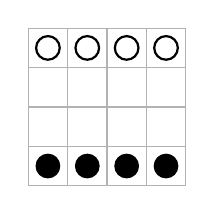
\begin{tikzpicture}[scale=0.50]
\draw[step=1,black!30] (0,0) grid (4,4);
\filldraw[white,draw=black,thick] (0.5,3.5) circle (0.30);
\filldraw[white,draw=black,thick] (1.5,3.5) circle (0.30);
\filldraw[white,draw=black,thick] (2.5,3.5) circle (0.30);
\filldraw[white,draw=black,thick] (3.5,3.5) circle (0.30);
\filldraw[black] (0.5,0.5) circle (0.30);
\filldraw[black] (1.5,0.5) circle (0.30);
\filldraw[black] (2.5,0.5) circle (0.30);
\filldraw[black] (3.5,0.5) circle (0.30);

\end{tikzpicture}
\caption{The initial position $s_0^\bl$ (\S3). Black ($\bullet$) is to move.}
\end{figure}

\begin{definition}[plain moves]
The set of \emph{plain moves} at $s$ is
$\Mv(s)=\{(x,y): x\in P(s),\; y\notin B\cup W,\; d_1(x,y)=1\}$ (\S6). For
$m=(x,y)\in\Mv(s)$ put $P'=\bigl(P(s)\setminus\{x\}\bigr)\cup\{y\}$.
\end{definition}

Captures are not declared by the player; they are detected automatically after the move,
and only on the two lines through the destination square (\S7.1).

\begin{definition}[capture candidates]\label{def:cap}
Let $m=(x,y)\in\Mv(s)$, $Q=Q(s)$ and let $L$ be one of the two lines containing $y$. A
square $z$ is a \emph{capture candidate on $L$} if, writing $O_L=(P'\cup Q)\cap L$
(\S7.2),
\begin{enumerate}[label=(\roman*),itemsep=1pt,topsep=2pt]
\item $|O_L|=3$; \quad (ii) $|P'\cap L|=2$; \quad (iii) $Q\cap L=\{z\}$;
\setcounter{enumi}{3}
\item writing $P'\cap L=\{a,b\}$, one has $d_1(a,b)=1$;
\item $d_1(z,a)=1$ or $d_1(z,b)=1$.
\end{enumerate}
Write $\Zc(s,m)$ for the set of capture candidates on either of the two lines through $y$.
\end{definition}

Thus a capture occurs precisely when the move creates, on a line through the destination,
a configuration of exactly three men consisting of two adjacent men of the mover and one
adjacent man of the opponent --- a sandwich seen from one side, whence the name. Since
$y\in P'\cap L$, the moved man is automatically one of $a,b$.

\begin{figure}[h]
\centering
\begin{tabular}{ccccc}
\input{fig_cap_ok1} & \input{fig_cap_ok2} & \input{fig_cap_no1} & \input{fig_cap_no2} & 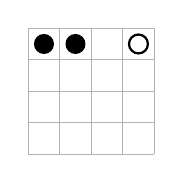
\begin{tikzpicture}[scale=0.40]
\draw[step=1,black!30] (0,0) grid (4,4);
\filldraw[black] (0.5,3.5) circle (0.30);
\filldraw[black] (1.5,3.5) circle (0.30);
\filldraw[white,draw=black,thick] (3.5,3.5) circle (0.30);

\end{tikzpicture}\\
capture & capture & no ($a,b$ apart) & no ($|O_L|=4$) & no ($z$ not adjacent)
\end{tabular}
\caption{Line patterns for Black to move, after Black's man has arrived on the line
(\S7.3--7.4). Only the row and the column through the destination square are examined.}
\end{figure}

\begin{definition}[actions]
The set of \emph{actions} at $s$ is
\[
 \Act(s)=\bigl\{(m,z): m\in\Mv(s),\, z\in\Zc(s,m)\bigr\}
      \;\cup\;\bigl\{(m,\bot): m\in\Mv(s),\, \Zc(s,m)=\emptyset\bigr\}.
\]
\end{definition}

Capturing is mandatory (\S8): if $\Zc(s,m)\neq\emptyset$ the mover \emph{must} remove one
candidate, and if there are two candidates the mover chooses which (\S8.3). At most one
man is captured per turn and chain captures are forbidden (\S8.4--8.5). Since every plain
move yields at least one action, we record:

\begin{equation}\label{eq:actempty}
  \Act(s)=\emptyset \iff \Mv(s)=\emptyset .
\end{equation}

\begin{definition}[transition]
Let $a=(m,z)\in\Act(s)$ with $m=(x,y)$. Put $Q'=Q(s)\setminus\{z\}$ if $z\neq\bot$ and
$Q'=Q(s)$ otherwise. If $|Q'|=2$ we call $a$ \emph{winning} and write
$s\cdot a=\wins$. Otherwise $s\cdot a\in\St$ is the position with mover's set $P'$,
opponent's set $Q'$ and the other side to move.
\end{definition}

\subsection{Plays, termination, and the repetition rule}

\begin{definition}[plays]
A \emph{play} from $s_0\in\St$ is a finite sequence
$\pi=(s_0,a_0,s_1,a_1,\dots)$ with $a_k\in\Act(s_k)$ and $s_{k+1}=s_k\cdot a_k\in\St$,
which ends in exactly one of the following three ways. Let $H_k=(s_0,\dots,s_k)$ and let
$\mathrm{occ}_{H_k}(s)$ be the number of indices $j\le k$ with $s_j=s$. Immediately after
the mover at $s_k$ has chosen $a_k$, the following tests are applied \emph{in this order}
(\S11.4):
\begin{enumerate}[label=(T\arabic*),itemsep=1pt,topsep=2pt]
\item if $a_k$ is winning, the play ends and the mover at $s_k$ \textbf{wins} (\S8, \S9);
\item otherwise $s_{k+1}=s_k\cdot a_k$ is appended, and if $\Mv(s_{k+1})=\emptyset$ the
play ends and the mover at $s_{k+1}$ \textbf{loses} (\S10);
\item otherwise, if $\mathrm{occ}_{H_{k+1}}(s_{k+1})=3$ the play ends in a
\textbf{draw} (\S11.2).
\end{enumerate}
If none of (T1)--(T3) applies, play continues from $s_{k+1}$. Test (T2) is also applied
to $s_0$ itself before the first move.
\end{definition}

Two features of this definition deserve emphasis. First, the object counted for
repetition is the \emph{full position} $(B,W,t)$, not the board pattern (\S11.1), and the
initial position counts as its own first occurrence (\S11.2). Second, the priority order
matters: a player who is immobilised loses even if the position is simultaneously a third
repetition (\S11.4).

Because termination depends on the history, a strategy is in general a function of
histories, not of positions, and the rules document explicitly warns (\S17) that an exact
analysis must use the extended state $(B,W,t,H)$. The following elementary observation
removes the difficulty for our purposes.

\begin{lemma}[finiteness]\label{lem:finite}
Every play from any $s_0\in\St$ has at most $2N+1$ moves, where $N=|\St|=\Npos$. In
particular the game is finite, and every maximal play ends by one of \textup{(T1)},
\textup{(T2)}, \textup{(T3)}.
\end{lemma}

\begin{proof}
Say that a position is \emph{appended} when it is added to the history; $s_0$ counts as
appended once, and each move either ends the play by (T1) or appends exactly one position.
Hence, if the play has $\ell$ moves, the number of appendings is $\ell$ or $\ell+1$; in
either case $\ell$ does not exceed the number of appendings.

Suppose some position reaches three appendings, say $s_{k+1}$ with
$\mathrm{occ}_{H_{k+1}}(s_{k+1})=3$. Then the play ends at that point: (T1) has already
been passed, so if (T2) does not fire, (T3) does. Consequently at most one position is
appended three times and it is the last appending, while every other position is appended
at most twice. The number of appendings is therefore at most $2(N-1)+3=2N+1$, and so is
the number of moves.

Finally, if a play has not ended at $s_k$ then $\Mv(s_k)\neq\emptyset$ by (T2), hence
$\Act(s_k)\neq\emptyset$ by~\eqref{eq:actempty} and the mover has an action available. So
a maximal play cannot go on forever and cannot get stuck without a verdict: it ends, and
only by (T1)--(T3).
\end{proof}

\begin{remark}
The bound $2N+1$ is of course absurdly pessimistic --- the longest line observed in the
auxiliary history-free analysis is shorter than $30$ moves --- but its only role is to
guarantee that no play is infinite. It does not by itself imply that positional strategies
suffice for a history-dependent game. For the strategies constructed below, that conclusion
comes from Theorem~\ref{thm:sound}: the repetition rule can only ever \emph{add} a draw
termination, never a loss, so a strategy certified not to lose on any finite prefix never
loses at all.
\end{remark}

\section{Safety certificates}\label{sec:safety}

Throughout, $P\in\{\text{Black},\text{White}\}$ is a distinguished player and $\bar P$ is
the opponent. We say a position $s$ is \emph{$P$-to-move} if $t=\bl$ and $P$ is Black, or
$t=\wh$ and $P$ is White.

\begin{definition}[$P$-safe set]\label{def:safe}
A set $S\subseteq\St$ is \emph{$P$-safe} if
\begin{enumerate}[label=(S\arabic*),itemsep=2pt,topsep=3pt]
\item for every $P$-to-move $s\in S$ there exists $a\in\Act(s)$ such that $a$ is winning
or $s\cdot a\in S$;
\item for every $\bar P$-to-move $s\in S$ and every $a\in\Act(s)$: $a$ is not winning,
and $s\cdot a\in S$.
\end{enumerate}
\end{definition}

Both conditions are local: (S1) quantifies over the actions at a single position and (S2)
likewise, and membership in $S$ is a table lookup. Note that (S1) forces
$\Act(s)\neq\emptyset$, hence $\Mv(s)\neq\emptyset$ by~\eqref{eq:actempty}, so a
$P$-to-move position of a $P$-safe set is never immobile. Condition (S2) is vacuous at a
$\bar P$-to-move position with $\Act(s)=\emptyset$; such a position is a win for $P$
by (T2).

A \emph{positional} (or memoryless) strategy for $P$ is a map $\sigma$ assigning to each
$P$-to-move position $s$ with $\Act(s)\ne\emptyset$ an action $\sigma(s)\in\Act(s)$; a play
is \emph{consistent with $\sigma$} if $P$'s every action is given by $\sigma$.

\begin{theorem}[soundness]\label{thm:sound}
Let $S$ be $P$-safe and $s_0\in S$. Then there is a positional strategy $\sigma$ for $P$
such that every maximal play from $s_0$ consistent with $\sigma$ ends either with a win
for $P$ by \textup{(T1)} or \textup{(T2)}, or in a draw by \textup{(T3)}. In particular
$\bar P$ has no winning strategy from $s_0$, and $P$ has a strategy guaranteeing at least
a draw.
\end{theorem}

\begin{proof}
For each $P$-to-move $s\in S$ choose, using (S1), an action $\sigma(s)\in\Act(s)$ that is
winning or satisfies $s\cdot\sigma(s)\in S$ (a choice from finitely many finite sets);
define $\sigma$ arbitrarily outside $S$. Let $\pi$ be a maximal play from $s_0$ consistent
with $\sigma$.

We claim that every position appended in $\pi$ lies in $S$, and that $\pi$ does not end
with a win for $\bar P$. We argue by induction along $\pi$; the base case $s_0\in S$ is the
hypothesis. Let $s_k\in S$ and suppose the play has not yet ended at $s_k$.

If $s_k$ is $P$-to-move, then $\Mv(s_k)\ne\emptyset$ as observed above, so the play was not
ended by (T2) at $s_k$ for want of a move. $P$ plays $\sigma(s_k)$: either it is winning,
and $\pi$ ends with a win for $P$ by (T1); or $s_{k+1}=s_k\cdot\sigma(s_k)\in S$ and the
play either ends by (T2) --- which is then a loss for the mover at $s_{k+1}$, i.e.\ for
$\bar P$, a win for $P$ --- or by (T3) as a draw, or continues.

If $s_k$ is $\bar P$-to-move, then either $\Mv(s_k)=\emptyset$, in which case $\pi$ already
ended by (T2) with a loss for $\bar P$; or $\bar P$ plays some $a\in\Act(s_k)$. By (S2)
$a$ is not winning, so $\pi$ does not end by (T1) here, and $s_{k+1}=s_k\cdot a\in S$. As
before the play may then end by (T2) (a loss for the mover at $s_{k+1}$, i.e.\ for $P$ ---
but this is impossible, since $s_{k+1}\in S$ is $P$-to-move and hence not immobile), or by
(T3) as a draw, or continue.

This proves the claim. By Lemma~\ref{lem:finite} the play $\pi$ is finite, and being
maximal it ends by one of (T1)--(T3); by the claim the only possibilities are a win for
$P$ or a draw.
\end{proof}

\begin{remark}[why a greatest fixed point]
The union of two $P$-safe sets is $P$-safe, so there is a largest one, $S^\ast_P$; it is
the greatest fixed point of the monotone operator $F(S)=\{s: \text{(S1) or (S2) holds for
$s$ w.r.t.\ } S\}$ and can be computed by iterated deletion from $\St$ (Tarski
\cite{tarski}; see \cite{gtw} for safety games). $S^\ast_P$ is the exact non-losing
region for the history-free safety objective defined by \textup{(S1)}--\textup{(S2)}.
For the actual game, whose repetition rule is history-sensitive, it is a certified subset
of that game's non-losing region. The point of Definition~\ref{def:safe} is not the existence but
the \emph{form}: any $S$ whatsoever, however obtained, proves the theorem once (S1) and
(S2) are checked, and the check never mentions the iteration that produced $S$.
\end{remark}

\begin{remark}[complexity of checking]
Verifying (S1)--(S2) for a given $S\subseteq\St$ costs one pass over $\St$, generating the
actions of each position; with a bitboard representation of $B$ and $W$ this is
$O(N)$ time and $O(N)$ space with tiny constants. Our verifier
(Section~\ref{sec:verify}) does it in $0.12$~s.
\end{remark}

\section{The symmetries of the rules}\label{sec:sym}

Let
\[
 \mu(r,c)=(r,5-c),\qquad \tau(r,c)=(5-r,5-c).
\]
Both are involutive bijections of $X$; $\mu$ is the left--right mirror and $\tau$ the
$180^\circ$ rotation. We extend them to sets of squares elementwise, and define
\[
 \hat\mu(B,W,t)=(\mu B,\mu W,t),\qquad
 \boxed{\;\rho(B,W,t)=(\tau W,\tau B,\bar t)\;}
\]
where $\bar\bl=\wh$ and $\bar\wh=\bl$. Thus $\rho$ rotates the board, exchanges the
colours, and exchanges the side to move.

\begin{lemma}\label{lem:rho}
$\rho$ is an involution of $\St$, and for every $s\in\St$ there is a bijection
$\Act(s)\to\Act(\rho s)$, $a\mapsto \rho_s a$, such that
\begin{enumerate}[label=(\roman*),itemsep=1pt,topsep=2pt]
\item $a$ is winning if and only if $\rho_s a$ is winning;
\item if $a$ is not winning then $\rho(s\cdot a)=\rho s\cdot \rho_s a$;
\item $\Act(s)=\emptyset$ if and only if $\Act(\rho s)=\emptyset$.
\end{enumerate}
The same holds with $\hat\mu$ in place of $\rho$.
\end{lemma}

\begin{proof}
That $\rho$ is an involution of $\St$ is immediate: $\tau$ is a bijection preserving
disjointness and cardinality, and $\bar{\bar t}=t$.

The mover's set at $s$ is $P(s)$, and the mover's set at $\rho s$ is
$\tau P(s)$: if $t=\bl$ then $P(s)=B$, and the side to move at $\rho s$ is $\wh$ whose set
is $\tau B$; symmetrically for $t=\wh$. Likewise the opponent's set at $\rho s$ is
$\tau Q(s)$. So $\rho$ maps the mover to the mover and the opponent to the opponent.

Now $\tau$ is an automorphism of the grid graph on $X$: it is a bijection with
$d_1(\tau u,\tau v)=d_1(u,v)$. It also permutes the eight lines, since
$\tau R_r=R_{5-r}$ and $\tau C_c=C_{5-c}$, and it maps the two lines through $y$ onto the
two lines through $\tau y$. Define $\rho_s(x,y)=(\tau x,\tau y)$ on plain moves; by the
above this is a bijection $\Mv(s)\to\Mv(\rho s)$, and it maps $P'$ to $(\tau P)'$.
Conditions (i)--(v) of Definition~\ref{def:cap} mention only cardinalities of intersections
of $P'$ and $Q$ with a line and $d_1$-adjacencies between the men on that line; all of
these are preserved. Hence $\tau\Zc(s,m)=\Zc(\rho s,\rho_s m)$, and setting
$\rho_s(m,z)=(\rho_s m,\tau z)$ (with $\tau\bot=\bot$) gives a bijection
$\Act(s)\to\Act(\rho s)$. Since $|\tau Q'|=|Q'|$, an action is winning iff its image is,
which is (i); and (ii) holds by construction, because the image position has mover's set
$\tau P'$, opponent's set $\tau Q'$ and the opposite side to move, which is precisely
$\rho(s\cdot a)$. Finally (iii) follows from~\eqref{eq:actempty} and the bijection on
plain moves. The argument for $\hat\mu$ is identical, using that $\mu$ is a grid
automorphism permuting the lines and that $\hat\mu$ preserves colours.
\end{proof}

\begin{corollary}\label{cor:transfer}
If $S$ is Black-safe then $\rho(S)$ is White-safe, and conversely. If $S$ is $P$-safe
then so is $\hat\mu(S)$.
\end{corollary}

\begin{proof}
Let $S$ be Black-safe and put $S'=\rho(S)$; note $\rho$ maps Black-to-move positions to
White-to-move positions and conversely. Let $s'=\rho s\in S'$ be White-to-move, so $s\in
S$ is Black-to-move; by (S1) there is $a\in\Act(s)$ winning or with $s\cdot a\in S$, and
then $\rho_s a\in\Act(s')$ is winning, resp.\ satisfies
$s'\cdot\rho_sa=\rho(s\cdot a)\in S'$, by Lemma~\ref{lem:rho}. This is (S1) for $S'$ with
$P=$ White. Let $s'=\rho s\in S'$ be Black-to-move and $a'\in\Act(s')$; then
$a'=\rho_s a$ for a unique $a\in\Act(s)$ (using $\rho^2=\mathrm{id}$), $a$ is not winning
by (S2) for $S$, hence neither is $a'$, and $s'\cdot a'=\rho(s\cdot a)\in S'$. This is
(S2). The converse and the $\hat\mu$ statement are proved the same way.
\end{proof}

The following triviality is what couples the two colours.

\begin{lemma}\label{lem:init}
$\rho(s_0^\wh)=s_0^\bl$ and $\rho(s_0^\bl)=s_0^\wh$.
\end{lemma}

\begin{proof}
$\tau W_0=\tau\{\sqn{11},\sqn{12},\sqn{13},\sqn{14}\}
=\{\sqn{44},\sqn{43},\sqn{42},\sqn{41}\}=B_0$ and likewise $\tau B_0=W_0$; and
$\bar\wh=\bl$. Hence $\rho(B_0,W_0,\wh)=(\tau W_0,\tau B_0,\bl)=(B_0,W_0,\bl)$.
\end{proof}

\begin{remark}
This is the precise sense in which Three-Piece Siege is a \emph{symmetric} game: the two
players face the same problem, but with the side to move swapped. Consequently a single
certificate that contains the initial board \emph{both} with Black to move and with White
to move settles both colours at once. It is not a priori clear that such a certificate
exists: it asserts that Black can survive even after conceding the first move.
\end{remark}

\section{The certificate}\label{sec:cert}

\subsection{Statement}

We exhibit a set $S\subseteq\St$ of size $\Ncert$. It is given as a flat array of
one-byte flags indexed by $(\mathrm{rank}(B),\mathrm{rank}(W),t)$, where $\mathrm{rank}$
enumerates the $2380$ subsets of $X$ of size $3$ or $4$ in increasing order of their
$16$-bit characteristic words (bit $i$ set iff square $i$, in row-major order, is
occupied); precisely, byte $(\mathrm{rank}(B)\cdot2380+\mathrm{rank}(W))\cdot2+t$ of the
file is $1$ if $(B,W,t)\in S$ and $0$ otherwise (this is the function \texttt{sidx} of
\texttt{engine.py}). The file \texttt{safe6.bin} of $2380^2\cdot2=11\,328\,800$ bytes is
part of the supplementary material; Section~\ref{sec:repro} gives its checksum and the
environment needed to regenerate it. Its statistics are
\[
\begin{gathered}
|S|=\Ncert,\\
\text{Black to move: }\NcertB,\qquad\text{White to move: }\NcertW,\\[2pt]
(|B|,|W|)=(4,4):\ \NcertFF,\qquad (4,3):\ \NcertFT,\\
(3,4):\ \NcertTF,\qquad (3,3):\ \NcertTT.
\end{gathered}
\]

\begin{theorem}\label{thm:cert}
$S$ is Black-safe, and $s_0^\bl\in S$ and $s_0^\wh\in S$.
\end{theorem}

The proof is a finite verification, described and audited in Section~\ref{sec:verify}.

\begin{theorem}[main]\label{thm:main}
Three-Piece Siege on the $4\times4$ board, with the rules of Section~\ref{sec:game}, is a
draw: each player has a positional strategy that guarantees at least a draw. Moreover any
maximal play in which one of these strategies is followed, and which is not won by the
player following it, ends in a draw by threefold repetition after at most $2N+1$ moves.
\end{theorem}

\begin{proof}
By Theorem~\ref{thm:cert}, $S$ is Black-safe and $s_0^\bl\in S$; by
Theorem~\ref{thm:sound} with $P=$~Black, Black has a positional strategy guaranteeing at
least a draw from $s_0^\bl$, and White has no winning strategy.

By Theorem~\ref{thm:cert} and Corollary~\ref{cor:transfer}, $S'=\rho(S)$ is White-safe.
By Theorem~\ref{thm:cert} again, $s_0^\wh\in S$, so by Lemma~\ref{lem:init}
$s_0^\bl=\rho(s_0^\wh)\in S'$. By Theorem~\ref{thm:sound} with $P=$~White, White has a
positional strategy guaranteeing at least a draw from $s_0^\bl$, and Black has no winning
strategy. The bound on the length of a play is Lemma~\ref{lem:finite}.
\end{proof}

\begin{remark}
No appeal to Zermelo's theorem or to backward induction is made: both non-losing
strategies are exhibited, and ``draw'' means precisely that neither player has a winning
strategy while both have non-losing ones. In particular the argument is unaffected by the
history-dependence of (T3).
\end{remark}

\begin{remark}[the first-repetition variant]
Under the variant of \S13, in which the \emph{second} occurrence of a full position is
already a draw, Lemma~\ref{lem:finite} improves to $N+1$ moves and nothing else changes:
Definition~\ref{def:safe} and Theorem~\ref{thm:sound} never mention how many repetitions
are needed, only that a repetition draw is not a loss. Hence Theorem~\ref{thm:main} holds
verbatim for that variant, with the same certificate $S$ and the same strategies.
\end{remark}

\subsection{Where $S$ came from}

The construction is heuristic and plays no part in the proof; we record it for
reproducibility. Starting from the full state space we compute the greatest fixed point of
the safety operator for Black by iterated deletion (program \texttt{safety6.c}: $24$
sweeps, $0.19$~s). This yields the largest Black-safe set, which is huge and structureless.
To obtain something intelligible we restrict Black's admissible shapes: fix the
$10$-square region
\[
 \Rg=\{\sqn{22},\sqn{23}\}\cup R_3\cup R_4
\]
and a whitelist $\mathcal{W}$ of subsets of $\Rg$ of size $3$ or $4$, and compute the
greatest fixed point of the safety operator \emph{restricted} to positions with
$B\in\mathcal{W}$ --- that is, Black must at every moment be able to keep his men inside
the whitelist. The whitelist is then minimised greedily: shapes (in $\hat\mu$-orbits, to
keep the result mirror-symmetric) are proposed for deletion in order of decreasing
distance from Black's home block, and a deletion is accepted if the restricted fixed point
still contains \emph{both} $s_0^\bl$ and $s_0^\wh$ (program \texttt{prune3.py}, $170$
orbit trials, each a full re-solve). The surviving whitelist has $\Nshapes$ shapes and the
associated fixed point is $S$.

\begin{figure}[h]
\centering
\begin{tabular}{ccc}
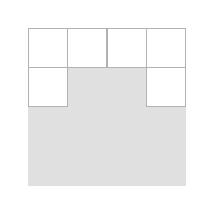
\begin{tikzpicture}[scale=0.50]
\draw[step=1,black!30] (0,0) grid (4,4);
\fill[black!12] (1.0,2.0) rectangle (2.0,3.0);
\fill[black!12] (2.0,2.0) rectangle (3.0,3.0);
\fill[black!12] (0.0,1.0) rectangle (1.0,2.0);
\fill[black!12] (1.0,1.0) rectangle (2.0,2.0);
\fill[black!12] (2.0,1.0) rectangle (3.0,2.0);
\fill[black!12] (3.0,1.0) rectangle (4.0,2.0);
\fill[black!12] (0.0,0.0) rectangle (1.0,1.0);
\fill[black!12] (1.0,0.0) rectangle (2.0,1.0);
\fill[black!12] (2.0,0.0) rectangle (3.0,1.0);
\fill[black!12] (3.0,0.0) rectangle (4.0,1.0);

\end{tikzpicture} & \qquad & 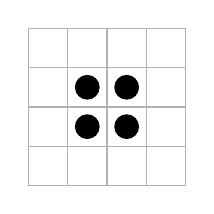
\begin{tikzpicture}[scale=0.50]
\draw[step=1,black!30] (0,0) grid (4,4);
\filldraw[black] (1.5,2.5) circle (0.30);
\filldraw[black] (2.5,2.5) circle (0.30);
\filldraw[black] (1.5,1.5) circle (0.30);
\filldraw[black] (2.5,1.5) circle (0.30);

\end{tikzpicture}\\
the region $\Rg$ & & the fortress
\end{tabular}
\caption{Left: the $10$ squares of $\Rg$; Black's men never leave this region in the
certificate (Proposition~\ref{prop:region}). Right: the central $2\times2$ block, the
unique four-man shape that is safe against every opposing configuration
(Proposition~\ref{prop:fortress}).}
\end{figure}

\subsection{Structure of $S$}

The following propositions report exhaustive checks over $S$. They are not needed for
Theorem~\ref{thm:main}, but they make the certificate readable.

\begin{proposition}[localisation]\label{prop:region}
For every $(B,W,t)\in S$ we have $B\subseteq\Rg$, where $|\Rg|=10$. Only $\Nshapes$ of the
$\Nregionshapes$ subsets of $\Rg$ of size $3$ or $4$ occur as such a $B$ --- $\Nshapesfour$
of size $4$ and $\Nshapesthree$ of size $3$ --- namely $\Nshapescanon$ up to the mirror
$\mu$. Moreover $S$ is $\hat\mu$-invariant. No condition is imposed on $W$: each of the
$\Nshapes$ shapes occurs in $S$ with between $\Nwcfgmin$ and $\Nwcfgmax$ different White
configurations.
\end{proposition}

\begin{remark}
Black's men never form the central block $B^\ast$ of Proposition~\ref{prop:fortress} in
this particular certificate: the minimisation deleted that shape from the whitelist.
This is a fact about the certificate's local structure only. It does not establish whether
either player can force occupation of the block, or force the other player away from it,
from the initial position; those reachability claims require a separate proof. The region
$\Rg$ is the neighbourhood of Black's \emph{half} of the centre, not the centre itself.
\end{remark}

\begin{proposition}[one exchange, and only one]\label{prop:exchange}
Let $(B,W,\wh)\in S$.
\begin{enumerate}[label=(\roman*),itemsep=1pt,topsep=2pt]
\item If $|B|=3$ then $\Zc\bigl((B,W,\wh),m\bigr)=\emptyset$ for every $m\in\Mv$: White
has no capturing move at all. This holds for all $\NlayerthreeW$ such positions in $S$.
\item If $|B|=4$, then of the $\NlayerfourW$ such positions in $S$ exactly $\Nbaitpos$
admit a capturing move for White, and in every one of them every White capture leads to a
position of $S$ with $|B|=3$ (in particular no White capture is winning).
\end{enumerate}
\end{proposition}

\begin{corollary}
In any play from $s_0^\bl$ in which Black follows a strategy witnessing (S1) for $S$,
White captures at most one Black man in the entire game, and Black is never reduced below
three men. Symmetrically for White.
\end{corollary}

\begin{proof}
By the proof of Theorem~\ref{thm:sound} every position of the play lies in $S$. Black's
men can only decrease, and by Proposition~\ref{prop:exchange}(i) once $|B|=3$ no White
move captures ever again; by (ii) the transition from $|B|=4$ to $|B|=3$ is not a win for
White.
\end{proof}

Thus the certificate encodes a two-layer defence. On the upper layer ($|B|=4$) Black
tolerates White's capturing chances but only ever offers \emph{bait}: every capture
White can make transports the game into the lower layer, where --- and this is the
substantive content --- White's captures have been extinguished for good. Black's own
winning chances are not renounced: of the positions reachable when Black follows the
explicit rule book of Section~\ref{sec:book}, $\NsigmaBwin$ are decisions in which
Black's book move wins outright.

\section{Verification}\label{sec:verify}

Theorem~\ref{thm:cert} is proved by the program \texttt{certify.c} ($232$ lines of C, no
dependencies). It reads the certificate file and performs a single pass over all
$\Npos$ positions, checking four conditions. Nothing is iterated and no game values are
consulted.

\begin{description}[itemsep=2pt,topsep=3pt,leftmargin=3.4em]
\item[(C1)] \emph{Legality.} Every $s$ with $s\in S$ satisfies $B\cap W=\emptyset$ and
$|B|,|W|\in\{3,4\}$, i.e.\ $S\subseteq\St$.
\item[(C2)] \emph{Black-safety.} For every Black-to-move $s\in S$, some action is winning
or stays in $S$; for every White-to-move $s\in S$, no action is winning and all actions
stay in $S$. (Definition~\ref{def:safe} with $P=$~Black.)
\item[(C3)] \emph{Initial positions.} $s_0^\bl\in S$ and $s_0^\wh\in S$.
\item[(C4)] \emph{White-safety of the transferred set.} Independently of
Corollary~\ref{cor:transfer}, the program forms $T=\{s_0^\bl\}\cup\rho(S)$ --- membership
in $T$ is decided on the fly by $s\in T\iff \rho s\in S$ or $s=s_0^\bl$, since
$\rho^2=\mathrm{id}$ --- and checks Definition~\ref{def:safe} for $T$ with $P=$~White.
\end{description}

Check (C4) is logically redundant given (C2), (C3) and Corollary~\ref{cor:transfer}, whose
proof is a page of routine verification; we include it so that the symmetry argument is
also machine-checked. The output on \texttt{safe6.bin} is

\begin{center}\small
\begin{tabular}{@{}lr@{}}
\toprule
$|S|$ & $\Ncert$\\
Black shapes occurring in $S$ & $\Nshapes$\\
$|T|=|\{s_0^\bl\}\cup\rho(S)|$ & $\Ncert$\\
(C1) illegal states in $S$ & $0$\\
(C2) Black-safety violations & $0$\\
(C3) $s_0^\bl\in S$ and $s_0^\wh\in S$ & yes\\
(C4) White-safety violations for $T$ & $0$\\
\midrule
running time & $0.12$~s\\
\bottomrule
\end{tabular}
\end{center}

That $|T|=|S|$ reflects $\hat\mu$- and $\rho$-compatibility of $S$ near the initial
position: $s_0^\bl$ already lies in $\rho(S)$ because $s_0^\wh\in S$.

The action generator inside \texttt{certify.c} implements Definition~\ref{def:cap}
directly from the rules text. The Python reference engine is covered by the published
unit tests in \texttt{test\_engine.py}. In particular, the verifier always enumerates
both capture candidates, so that (S2) quantifies over White's choice in the
two-candidate case (\S8.3) rather than fixing it.

\begin{remark}[what this verification does, and does not, establish]\label{rem:verif-scope}
\texttt{certify.c} checks the local certificate conditions, while
\texttt{test\_engine.py} tests the published Python reference implementation and
\texttt{verify\_dual.py} exhaustively checks the rule book in its two colour-conjugate
uses. This is not claimed to be cross-validation between two independent retrograde
solvers: the only retrograde program in the artifact is the auxiliary, history-free
\texttt{solve.c}. The remaining risk is a shared misunderstanding of the natural-language
rules or a defect in the verification programs. We have not obtained reproduction by an
independent third party, nor a specification of Definitions~\ref{def:cap}--\ref{def:safe}
in a proof assistant (Coq, Lean, Isabelle); either would reduce that residual risk.
\end{remark}

\section{A rule book that works for both colours}\label{sec:book}

A certificate proves that a non-losing strategy exists and, via (S1), implicitly encodes
one; but ``look up $\Ncert$ bits'' is not a strategy a person can follow. We now give an
explicit finite object.

\subsection{The language}

Let $\mathcal{K}$ be the following set of atomic predicates, each a function of the
opponent's set $W$ (and, for the last two, of $B$ as well), for a Black-to-move position
$(B,W,\bl)$:
\[
\begin{array}{ll}
 \text{$\mathsf{on}(u)$, $\mathsf{off}(u)$} & \text{the opponent does / does not occupy square $u$};\\
 \mathsf{count}(k) & |W|=k;\\
 \mathsf{row}_{\ge}(r,k),\ \mathsf{col}_{\ge}(c,k) & \text{line $r$ (resp.\ $c$) contains at least $k$ opponent men};\\
 \mathsf{row}_{0}(r),\ \mathsf{col}_{0}(c) & \text{line $r$ (resp.\ $c$) contains no opponent man};\\
 \mathsf{thr},\ \mathsf{nthr} & \text{the opponent does / does not have a capturing move}.
\end{array}
\]
A \emph{rule book} is a finite partial map $\Pi$ from shapes $B\subseteq X$ to finite
sequences of \emph{items}, each item being either a \emph{candidate} $\langle m\rangle$
with $m$ a plain move, or a \emph{conditional} $\langle C\Rightarrow m\rangle$ with
$C\subseteq\mathcal{K}$ finite.

The book is executed as follows at a Black-to-move position $s=(B,W,\bl)$. First
$\hat\mu$-canonicalise: if $(\mu B,\mu W)$ precedes $(B,W)$ lexicographically, replace $s$
by $\hat\mu s$ and remember to mirror the answer back. Then look up the item sequence of
$B$ and scan it in order:
\begin{itemize}[itemsep=1pt,topsep=3pt]
\item a candidate $\langle m\rangle$ \emph{fires} if $m\in\Mv(s)$ and either the resulting
action wins or the resulting Black shape is one of the $\Nshapes$ shapes of $S$;
\item a conditional $\langle C\Rightarrow m\rangle$ fires if every predicate in $C$ holds
at $s$ (it is guaranteed by construction that then $m\in\Mv(s)$).
\end{itemize}
The move of the first item that fires is played, mirrored back if necessary. Finally, if
the chosen move has two capture candidates, the one on the larger row index is taken,
ties broken towards the smaller column index; this fixes the choice left open by \S8.3.

\begin{example}
Entry $\Nexentry$ of Appendix~\ref{app:book}, for the shape $\Nexcoords$, has
$\Nexrules$ items:

\begin{quote}\small
\noindent\textbf{Entry 29} \; 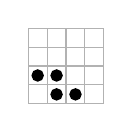
\begin{tikzpicture}[scale=0.24]
\draw[step=1,black!30] (0,0) grid (4,4);
\filldraw[black] (0.5,1.5) circle (0.30);
\filldraw[black] (1.5,1.5) circle (0.30);
\filldraw[black] (1.5,0.5) circle (0.30);
\filldraw[black] (2.5,0.5) circle (0.30);

\end{tikzpicture}
\nopagebreak\begin{enumerate}[topsep=1pt,itemsep=0pt,parsep=0pt,leftmargin=2.2em,label=\arabic*.]
\item if row 1 has >=2 opp and row 4 empty of opp: $31\!\to\!41$
\item if opp on 23 and col 4 has >=1 opp: $32\!\to\!33$
\item if opp on 21 and opp not on 41: $42\!\to\!41$
\item if col 3 empty of opp and row 1 has >=1 opp: $43\!\to\!33$
\item $31\!\to\!41$ \hfill\textit{(cand.)}
\item if opp not on 11 and opp not on 14: $32\!\to\!33$
\item $43\!\to\!44$ \hfill\textit{(cand.)}
\end{enumerate}\smallskip\end{quote}

\noindent Read top to bottom. Items $1$--$4$ and $6$ are exceptions triggered by specific
White placements; items $5$ and $7$ are the default plan --- retreat $\sqn{31}\to\sqn{41}$
if that is legal and keeps a recognised shape, otherwise shuffle $\sqn{43}\to\sqn{44}$ on
the bottom rank. The exceptions are listed before the default they override, which is why
a rule as unconditional-looking as item $5$ can appear in the middle of the list.
\end{example}

The size of the book we obtained is
\[
 \Nbookshapes \text{ entries},\qquad
 \Nbookcand \text{ candidates},\qquad
 \Nbookcond \text{ conditionals},\qquad
 \Nbookrules \text{ rules in total}.
\]
It is printed in full in Appendix~\ref{app:book}. The machine-readable book is the
supplementary file \texttt{book\_dual.pkl}, executed by the $130$-line interpreter
\texttt{dualbook.py}.

\subsection{Extraction}

Again the construction is irrelevant to the proof but we record it. We first compute, by
policy iteration inside $S$, for every Black-to-move $s\in S$ the set $G(s)$ of
\emph{good} actions --- those that win immediately or stay in $S$ --- and then look for a
small book whose behaviour is pointwise in $G$. This is a set-cover problem: a candidate
item $\langle m\rangle$ placed early in a shape's list covers all positions of that shape
at which $m$ is legal, shape-preserving and good; the remaining positions must be covered
by conditionals, which are grown greedily by adding the predicate of $\mathcal{K}$ that
covers the most residual positions without covering a position where the move is not good.
Iterating --- fit the book, recompute the set reachable when the book is followed, refit
--- converged after a handful of rounds to a book that needs no fallback, i.e.\ that
decides every position reachable under its own play.

\subsection{Correctness for both colours}

Let $\Pi$ be the book. For a White-to-move position $s$ define
$\Pi^\rho(s)=\rho_{s}^{-1}\bigl(\Pi(\rho s)\bigr)$; concretely, rotate the board by
$180^\circ$, exchange the colours, consult $\Pi$, and rotate the answer back. (The
capture preference is conjugated accordingly.)

\begin{theorem}\label{thm:book}
\begin{enumerate}[label=(\roman*),itemsep=2pt,topsep=3pt]
\item Following $\Pi$ from either $s_0^\bl$ or $s_0^\wh$, Black never loses: at every
reachable Black-to-move position the book returns a legal move, and at every reachable
White-to-move position no White action is winning. The set of positions reachable in this
way has $\Nsigma$ elements, of which $\NsigmaBdec$ are Black decisions and $\NsigmaWnodes$
are White-to-move; in $\NsigmaBwin$ of the decisions Black's move wins outright by reducing
White to two men; White is immobile in $\NsigmaBstuck$ of the reachable positions.
\item Following $\Pi^\rho$ from $s_0^\bl$, White never loses, in the same sense. The
reachable set has $\Nomega$ elements, $\NomegaWdec$ White decisions and $\NomegaBnodes$
Black-to-move positions, with $\NomegaWwin$ immediate White wins; Black is immobile in
$\NomegaWstuck$ of them.
\item The reachable set of (ii) is contained in the $\rho$-image of the reachable set of
(i).
\end{enumerate}
\end{theorem}

The verification (program \texttt{verify\_dual.py}) is a breadth-first expansion in which
the book's side plays its single move and the opponent's side branches over
\emph{all} actions, with assertions for legality, for the absence of a winning opposing
action, and for non-immobility. It is independent of \texttt{certify.c} and of the
certificate file: it consults only the book and the rules engine. As an additional
cross-check, each successor of a book move was looked up in the value table of
Section~\ref{sec:table} and never had value ``win for the opponent to move''
($0$ discrepancies out of $\NsigmaBdec+\NomegaWdec$).

The reachable set $\Sigma$ of Theorem~\ref{thm:book}(i) is by construction Black-safe:
Black's book move witnesses (S1), and the expansion over all White actions witnesses (S2).
Since $s_0^\bl,s_0^\wh\in\Sigma$ we obtain a second, sharper certificate, which we have
verified with the same program \texttt{certify.c}:

\begin{theorem}\label{thm:sigma}
The set $\Sigma$ of positions reachable when Black follows $\Pi$ from
$\{s_0^\bl,s_0^\wh\}$ has $|\Sigma|=\Nsigma$ elements, involves $\Nsigmashapes$ Black
shapes, and passes checks \textup{(C1)--(C4)}. Hence $\Sigma$ alone proves
Theorem~\ref{thm:main}, and the strategy witnessing it is the $\Nbookrules$-rule book of
Appendix~\ref{app:book}.
\end{theorem}

So the certificate can be taken to be $\Sigma$, which is $67\%$ smaller than $S$ and comes
with a human-executable witness; we retain $S$ because its shape catalogue is the object
from which the book was built, and because $S$ is $\hat\mu$-invariant, which $\Sigma$ need
not be.

\subsection{The canonical drawn game}

If both players follow the book --- Black using $\Pi$, White using $\Pi^\rho$ --- the game
is decided quickly.

\begin{proposition}\label{prop:game}
When Black plays $\Pi$ and White plays $\Pi^\rho$ from $s_0^\bl$, the play is
\begin{center}
\Ncanondrawgame
\end{center}
and is a draw by threefold repetition after $\Ndrawplies$ plies: the positions reached
after plies $\Nrepplies$ coincide.
\end{proposition}

No capture occurs: both sides advance a man to the third rank, bring a second man to the
centre, and then shuffle. This is the shape of optimal play in this game --- neither side
can force an exchange on favourable terms, so both consolidate around the centre and wait.
It also illustrates why the repetition rule, and not a capture-based termination
condition, is what ends the game.

\begin{remark}
All four of Black's opening moves preserve the draw, as do (by Lemma~\ref{lem:rho}) all
four of White's; so the initial position is not a delicate one. The delicacy is in the
middle game: of the $\NsigmaBdec$ Black decisions in $\Sigma$, $\Nsharp$ ($\Nsharppct$)
admit at least one legal move that loses on the spot, and only $\Ngoodpct$ of all the legal
actions available at these decisions are non-losing. This is why the book needs
$\Nbookcond$ conditionals: a plan that ignores White's exact placement will not survive.
\end{remark}

\section{Corroboration: an auxiliary history-free retrograde classification}\label{sec:table}

Although no part of Theorem~\ref{thm:main} depends on it, we computed an auxiliary
history-free retrograde classification as a sanity check on the certificate and to obtain
the local structural facts below. The program \texttt{solve.c} performs value iteration
over all $\Npos$ positions, assigning \emph{draw} to cycles, and reaches a fixed point in
$65$ sweeps and $13.7$~s. This classification is used only as corroboration and is not
claimed to solve the history-sensitive game exactly or to give its value under (T3).

\begin{center}\small
\begin{tabular}{@{}lrr@{}}
\toprule
value for the side to move & positions & share\\
\midrule
win  & $\Nwin$ & $56.3\%$\\
loss & $\Nlose$ & $28.3\%$\\
draw & $\Ndraw$ & $15.4\%$\\
\midrule
total & $\Npos$ & \\
\bottomrule
\end{tabular}
\end{center}

Both $s_0^\bl$ and $s_0^\wh$ receive the label \emph{draw}, in agreement with the
certificate theorem. Note how sharp this auxiliary classification is: more than five out
of six positions receive decisive labels, which is why a drawing strategy must be as
detailed as the book of Appendix~\ref{app:book}.

The table also explains \emph{why} the game is drawn.

\begin{proposition}[the fortress]\label{prop:fortress}
Among the $\Nfourshapesall$ four-man shapes $B\subseteq X$, exactly $\Nfortressnum$ has the
property that for every admissible opposing set $W$ Black does not lose, whether Black or
White is to move; namely the central block
$B^\ast=\{\sqn{22},\sqn{23},\sqn{32},\sqn{33}\}$. Its profile against the $495$ four-man
White sets disjoint from it is: Black to move, $\Nfortbwin$ wins, $\Nfortbdraw$ draws,
$\Nfortblose$ losses; White to move, $\Nfortwwin$ wins for White, $\Nfortwdraw$ draws,
$\Nfortwlose$ losses for White. Against the $220$ three-man White sets, Black to move
wins in all $\Nfortbwinth$, and White to move loses in all $\Nfortwloseth$.
\end{proposition}

In words: this is a local structural fact about positions in which a player already holds
the central $2\times2$ block with four men. By the symmetry of Lemma~\ref{lem:rho} the
corresponding fact holds for White. It does not imply that either player can force
occupation of that block, or force the other player away from it, from the initial
position; such reachability claims would require a separate proof. The certificate's
region $\Rg$ (Proposition~\ref{prop:region}) is a neighbourhood of Black's half of the
centre.

\section{Reproducibility}\label{sec:repro}

All programs required to verify the main certificate and executable rule book are in the
artifact and are self-contained (C99 and Python 3, no third-party libraries). Times are
from the reference run on one core of a commodity laptop.

\begin{center}\small
\begin{tabular}{@{}llrl@{}}
\toprule
file & rôle & lines & time\\
\midrule
\texttt{engine.py} & reference rules engine (bitboards) & $146$ & ---\\
\texttt{test\_engine.py} & unit tests for the reference engine & $107$ & $0.1$~s\\
\texttt{solve.c} & auxiliary history-free retrograde classification & $251$ & $13.7$~s\\
\texttt{safety6.c} & greatest fixed point inside a shape whitelist & $190$ & $0.19$~s\\
\texttt{prune3.py} & greedy minimisation of the whitelist ($170$ trials) & $72$ & $58$~s\\
\texttt{dualbook.py} & executable rule-book representation & $130$ & ---\\
\textbf{\texttt{certify.c}} & \textbf{the verifier: checks (C1)--(C4)} & $\mathbf{232}$ & $\mathbf{0.12}$~s\\
\texttt{verify\_dual.py} & exhaustive check of the book, both colours & $88$ & $0.9$~s\\
\bottomrule
\end{tabular}
\end{center}

\subsection{Data format}

Both \texttt{safe6.bin} and \texttt{sigma.bin} use the byte encoding given in
Section~\ref{sec:cert}: a file of $11\,328\,800$ bytes, one per triple
$(\mathrm{rank}(B),\mathrm{rank}(W),t)$, value $1$ for membership and $0$ otherwise, with
\[
 \texttt{sidx}(B,W,t)=(\mathrm{rank}(B)\cdot2380+\mathrm{rank}(W))\cdot2+t .
\]
\texttt{values.bin} has the same shape and indexing but one byte per \emph{pair}
$(\mathrm{rank}(B),\mathrm{rank}(W))$ doubled for the two values of $t$, encoding the
result of Section~\ref{sec:table} as $1=$~win, $2=$~loss, $3=$~draw for the side to move.
The rule book is a Python dictionary pickled to \texttt{book\_dual.pkl}, keyed by the
$16$-bit integer encoding of $B$, each value the ordered list of items of
Section~\ref{sec:book} in the internal representation consumed by \texttt{dualbook.py};
the same information is human-readable in Appendix~\ref{app:book} and is what the
$232$-line verifier never needs to touch. The book is a published, hash-checked
certificate: it is exhaustively verified by \texttt{verify\_dual.py}, but its compact
rule-fitting construction is not regenerated by the one-command script.

\subsection{Environment and checksums}

The reference run used CPython~3.10 and GCC~11.4 (\texttt{-O2}, C99, no non-standard
extensions) on x86-64 Linux; nothing in the code is platform-specific, and none of the
programs listed above links against a library beyond the standard ones shipped with Python
and a C compiler. The fixed-version artifact repository includes the source, certificate
files, \texttt{SHA256SUMS.txt}, \texttt{expected-output.txt}, and the one-command script
\texttt{scripts/verify.sh}. The release record must additionally name its repository
commit or tag and the exact clean-room environment. As a fixed reference point independent
of the prose descriptions, the certificate file used throughout has SHA-256 digest
\begin{center}
\footnotesize\ttfamily
sha256(safe6.bin)\\
6DA3BF4F72B850F0167DA092D26E180CDDA2B1D381EA0122F48850985D3B5581
\end{center}
and size $11\,328\,800$ bytes.
A different digest means that byte-for-byte regeneration was not reproduced; the theorem
must then be rechecked using the verifier. A digest difference alone does not refute the
theorem if the newly generated certificate passes that verification.

\subsection{Reproduction command}

To reproduce the proof of Theorem~\ref{thm:main} it suffices to compile and run
\begin{center}
\texttt{cc -O2 -o certify certify.c \&\& ./certify safe6.bin}
\end{center}
which reads the certificate and prints the four counts of the table in
Section~\ref{sec:verify}; the expected output is exactly that table (in particular, all
four violation counts are $0$ and (C3) reads \emph{yes}). Nothing else --- no solver, no
database, no search --- is involved. Running it on \texttt{sigma.bin} instead verifies
Theorem~\ref{thm:sigma}, with the corresponding counts of Section~\ref{sec:book}.
The certificate file itself is regenerated from scratch, without any of the other
artefacts, by \texttt{cc -O2 -o safety6 safety6.c \&\& FRESH=1 python3 prune3.py}, which
took $58$~s in the reference environment and should reproduce \texttt{safe6.bin} with the
recorded SHA-256 digest. An independent clean-room reproduction remains outstanding; its
record must give the exact environment, artifact commit, commands, digests, verifier
output, and result.

\section{Discussion}

The proof above has three ingredients of different natures, and it is worth separating
them. The \emph{mathematical} content is Lemma~\ref{lem:finite} (the repetition rule makes
the game finite), Theorem~\ref{thm:sound} (the safety certificate establishes that the
constructed positional strategies are non-losing), and Lemma~\ref{lem:rho} together with
Corollary~\ref{cor:transfer} and Lemma~\ref{lem:init} (the colour symmetry transfers a
certificate from one player to the other, and the initial position is a fixed point of the
transfer). The \emph{computational} content is a single pass of local checks over
$\Npos$ positions. The \emph{heuristic} content --- the search for a small, structured,
mirror-symmetric certificate and for a compact rule book --- is where all the work went,
and none of it needs to be trusted.

Several questions suggest themselves. Is there a certificate small enough to check by
hand? Proposition~\ref{prop:region} reduces Black's side of the state space to
$\Nshapescanon$ shapes, but each shape still carries thousands of White configurations, and
Proposition~\ref{prop:exchange} shows that the interaction with White's configuration
cannot be ignored. Our rule book needs $\Nbookcond$ conditionals, and we do not know the
minimum; the corresponding decision problem (is there a book of $\le k$ rules in a fixed
predicate language?) is a natural measure of a game's strategic complexity, and is
plausibly hard. A second question is scaling: how does the value of the game change on
$n\times n$ boards, or with $k$ men each, or if captures are allowed to chain? The
mandatory-capture rule makes material a liability as well as an asset --- one is sometimes
forced to capture into a fork --- and it would be interesting to know whether the
draw persists.

\appendix

The two appendices below are data, not argument: nothing in the proof of
Theorem~\ref{thm:main} depends on them (that proof needs only Theorem~\ref{thm:cert} and
Section~\ref{sec:verify}), and nothing in Theorem~\ref{thm:book} or~\ref{thm:sigma}
depends on the reader inspecting them either, since both are machine-checked in full. They
are included so that the certificate and the book are auditable by eye and not only by
program; a venue with strict length limits could equally well relegate both to the
supplementary material and keep only the worked Example of Section~\ref{sec:book} in the
printed text, which is the only illustrative material actually used in the argument.

\section{The shape catalogue}\label{app:shapes}

The $\Nshapescanon$ Black shapes occurring in the certificate $S$, up to the left--right
mirror $\mu$ (Proposition~\ref{prop:region}); shapes of four men first, then of three.

\noindent\makebox[\textwidth]{\begin{minipage}{2.0cm}\centering 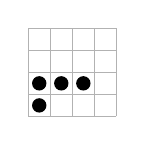
\begin{tikzpicture}[scale=0.28]
\draw[step=1,black!30] (0,0) grid (4,4);
\filldraw[black] (0.5,1.5) circle (0.30);
\filldraw[black] (1.5,1.5) circle (0.30);
\filldraw[black] (2.5,1.5) circle (0.30);
\filldraw[black] (0.5,0.5) circle (0.30);

\end{tikzpicture}\\[-1pt]{\tiny\#1}\end{minipage}\hfill\begin{minipage}{2.0cm}\centering 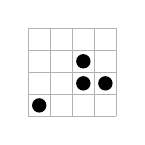
\begin{tikzpicture}[scale=0.28]
\draw[step=1,black!30] (0,0) grid (4,4);
\filldraw[black] (2.5,2.5) circle (0.30);
\filldraw[black] (2.5,1.5) circle (0.30);
\filldraw[black] (3.5,1.5) circle (0.30);
\filldraw[black] (0.5,0.5) circle (0.30);

\end{tikzpicture}\\[-1pt]{\tiny\#2}\end{minipage}\hfill\begin{minipage}{2.0cm}\centering 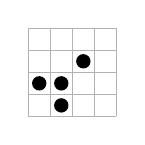
\begin{tikzpicture}[scale=0.28]
\draw[step=1,black!30] (0,0) grid (4,4);
\filldraw[black] (2.5,2.5) circle (0.30);
\filldraw[black] (0.5,1.5) circle (0.30);
\filldraw[black] (1.5,1.5) circle (0.30);
\filldraw[black] (1.5,0.5) circle (0.30);

\end{tikzpicture}\\[-1pt]{\tiny\#3}\end{minipage}\hfill\begin{minipage}{2.0cm}\centering 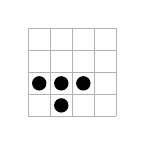
\begin{tikzpicture}[scale=0.28]
\draw[step=1,black!30] (0,0) grid (4,4);
\filldraw[black] (0.5,1.5) circle (0.30);
\filldraw[black] (1.5,1.5) circle (0.30);
\filldraw[black] (2.5,1.5) circle (0.30);
\filldraw[black] (1.5,0.5) circle (0.30);

\end{tikzpicture}\\[-1pt]{\tiny\#4}\end{minipage}\hfill\begin{minipage}{2.0cm}\centering 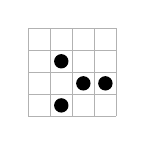
\begin{tikzpicture}[scale=0.28]
\draw[step=1,black!30] (0,0) grid (4,4);
\filldraw[black] (1.5,2.5) circle (0.30);
\filldraw[black] (2.5,1.5) circle (0.30);
\filldraw[black] (3.5,1.5) circle (0.30);
\filldraw[black] (1.5,0.5) circle (0.30);

\end{tikzpicture}\\[-1pt]{\tiny\#5}\end{minipage}\hfill\begin{minipage}{2.0cm}\centering 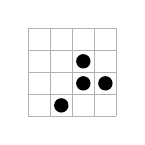
\begin{tikzpicture}[scale=0.28]
\draw[step=1,black!30] (0,0) grid (4,4);
\filldraw[black] (2.5,2.5) circle (0.30);
\filldraw[black] (2.5,1.5) circle (0.30);
\filldraw[black] (3.5,1.5) circle (0.30);
\filldraw[black] (1.5,0.5) circle (0.30);

\end{tikzpicture}\\[-1pt]{\tiny\#6}\end{minipage}}\par\vspace{6pt}
\noindent\makebox[\textwidth]{\begin{minipage}{2.0cm}\centering 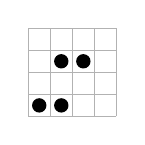
\begin{tikzpicture}[scale=0.28]
\draw[step=1,black!30] (0,0) grid (4,4);
\filldraw[black] (1.5,2.5) circle (0.30);
\filldraw[black] (2.5,2.5) circle (0.30);
\filldraw[black] (0.5,0.5) circle (0.30);
\filldraw[black] (1.5,0.5) circle (0.30);

\end{tikzpicture}\\[-1pt]{\tiny\#7}\end{minipage}\hfill\begin{minipage}{2.0cm}\centering 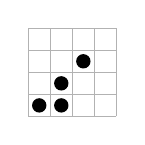
\begin{tikzpicture}[scale=0.28]
\draw[step=1,black!30] (0,0) grid (4,4);
\filldraw[black] (2.5,2.5) circle (0.30);
\filldraw[black] (1.5,1.5) circle (0.30);
\filldraw[black] (0.5,0.5) circle (0.30);
\filldraw[black] (1.5,0.5) circle (0.30);

\end{tikzpicture}\\[-1pt]{\tiny\#8}\end{minipage}\hfill\begin{minipage}{2.0cm}\centering 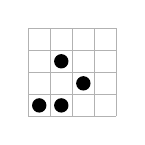
\begin{tikzpicture}[scale=0.28]
\draw[step=1,black!30] (0,0) grid (4,4);
\filldraw[black] (1.5,2.5) circle (0.30);
\filldraw[black] (2.5,1.5) circle (0.30);
\filldraw[black] (0.5,0.5) circle (0.30);
\filldraw[black] (1.5,0.5) circle (0.30);

\end{tikzpicture}\\[-1pt]{\tiny\#9}\end{minipage}\hfill\begin{minipage}{2.0cm}\centering 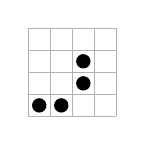
\begin{tikzpicture}[scale=0.28]
\draw[step=1,black!30] (0,0) grid (4,4);
\filldraw[black] (2.5,2.5) circle (0.30);
\filldraw[black] (2.5,1.5) circle (0.30);
\filldraw[black] (0.5,0.5) circle (0.30);
\filldraw[black] (1.5,0.5) circle (0.30);

\end{tikzpicture}\\[-1pt]{\tiny\#10}\end{minipage}\hfill\begin{minipage}{2.0cm}\centering 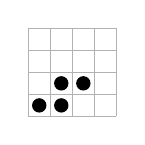
\begin{tikzpicture}[scale=0.28]
\draw[step=1,black!30] (0,0) grid (4,4);
\filldraw[black] (1.5,1.5) circle (0.30);
\filldraw[black] (2.5,1.5) circle (0.30);
\filldraw[black] (0.5,0.5) circle (0.30);
\filldraw[black] (1.5,0.5) circle (0.30);

\end{tikzpicture}\\[-1pt]{\tiny\#11}\end{minipage}\hfill\begin{minipage}{2.0cm}\centering 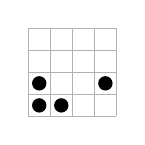
\begin{tikzpicture}[scale=0.28]
\draw[step=1,black!30] (0,0) grid (4,4);
\filldraw[black] (0.5,1.5) circle (0.30);
\filldraw[black] (3.5,1.5) circle (0.30);
\filldraw[black] (0.5,0.5) circle (0.30);
\filldraw[black] (1.5,0.5) circle (0.30);

\end{tikzpicture}\\[-1pt]{\tiny\#12}\end{minipage}}\par\vspace{6pt}
\noindent\makebox[\textwidth]{\begin{minipage}{2.0cm}\centering 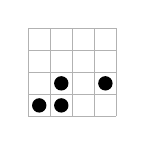
\begin{tikzpicture}[scale=0.28]
\draw[step=1,black!30] (0,0) grid (4,4);
\filldraw[black] (1.5,1.5) circle (0.30);
\filldraw[black] (3.5,1.5) circle (0.30);
\filldraw[black] (0.5,0.5) circle (0.30);
\filldraw[black] (1.5,0.5) circle (0.30);

\end{tikzpicture}\\[-1pt]{\tiny\#13}\end{minipage}\hfill\begin{minipage}{2.0cm}\centering 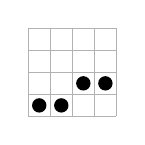
\begin{tikzpicture}[scale=0.28]
\draw[step=1,black!30] (0,0) grid (4,4);
\filldraw[black] (2.5,1.5) circle (0.30);
\filldraw[black] (3.5,1.5) circle (0.30);
\filldraw[black] (0.5,0.5) circle (0.30);
\filldraw[black] (1.5,0.5) circle (0.30);

\end{tikzpicture}\\[-1pt]{\tiny\#14}\end{minipage}\hfill\begin{minipage}{2.0cm}\centering 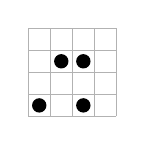
\begin{tikzpicture}[scale=0.28]
\draw[step=1,black!30] (0,0) grid (4,4);
\filldraw[black] (1.5,2.5) circle (0.30);
\filldraw[black] (2.5,2.5) circle (0.30);
\filldraw[black] (0.5,0.5) circle (0.30);
\filldraw[black] (2.5,0.5) circle (0.30);

\end{tikzpicture}\\[-1pt]{\tiny\#15}\end{minipage}\hfill\begin{minipage}{2.0cm}\centering 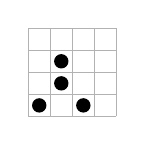
\begin{tikzpicture}[scale=0.28]
\draw[step=1,black!30] (0,0) grid (4,4);
\filldraw[black] (1.5,2.5) circle (0.30);
\filldraw[black] (1.5,1.5) circle (0.30);
\filldraw[black] (0.5,0.5) circle (0.30);
\filldraw[black] (2.5,0.5) circle (0.30);

\end{tikzpicture}\\[-1pt]{\tiny\#16}\end{minipage}\hfill\begin{minipage}{2.0cm}\centering 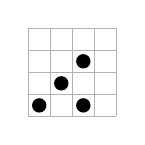
\begin{tikzpicture}[scale=0.28]
\draw[step=1,black!30] (0,0) grid (4,4);
\filldraw[black] (2.5,2.5) circle (0.30);
\filldraw[black] (1.5,1.5) circle (0.30);
\filldraw[black] (0.5,0.5) circle (0.30);
\filldraw[black] (2.5,0.5) circle (0.30);

\end{tikzpicture}\\[-1pt]{\tiny\#17}\end{minipage}\hfill\begin{minipage}{2.0cm}\centering 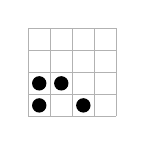
\begin{tikzpicture}[scale=0.28]
\draw[step=1,black!30] (0,0) grid (4,4);
\filldraw[black] (0.5,1.5) circle (0.30);
\filldraw[black] (1.5,1.5) circle (0.30);
\filldraw[black] (0.5,0.5) circle (0.30);
\filldraw[black] (2.5,0.5) circle (0.30);

\end{tikzpicture}\\[-1pt]{\tiny\#18}\end{minipage}}\par\vspace{6pt}
\noindent\makebox[\textwidth]{\begin{minipage}{2.0cm}\centering 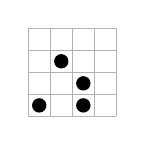
\begin{tikzpicture}[scale=0.28]
\draw[step=1,black!30] (0,0) grid (4,4);
\filldraw[black] (1.5,2.5) circle (0.30);
\filldraw[black] (2.5,1.5) circle (0.30);
\filldraw[black] (0.5,0.5) circle (0.30);
\filldraw[black] (2.5,0.5) circle (0.30);

\end{tikzpicture}\\[-1pt]{\tiny\#19}\end{minipage}\hfill\begin{minipage}{2.0cm}\centering 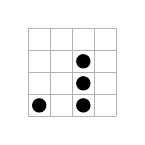
\begin{tikzpicture}[scale=0.28]
\draw[step=1,black!30] (0,0) grid (4,4);
\filldraw[black] (2.5,2.5) circle (0.30);
\filldraw[black] (2.5,1.5) circle (0.30);
\filldraw[black] (0.5,0.5) circle (0.30);
\filldraw[black] (2.5,0.5) circle (0.30);

\end{tikzpicture}\\[-1pt]{\tiny\#20}\end{minipage}\hfill\begin{minipage}{2.0cm}\centering 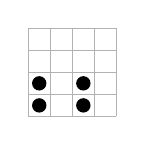
\begin{tikzpicture}[scale=0.28]
\draw[step=1,black!30] (0,0) grid (4,4);
\filldraw[black] (0.5,1.5) circle (0.30);
\filldraw[black] (2.5,1.5) circle (0.30);
\filldraw[black] (0.5,0.5) circle (0.30);
\filldraw[black] (2.5,0.5) circle (0.30);

\end{tikzpicture}\\[-1pt]{\tiny\#21}\end{minipage}\hfill\begin{minipage}{2.0cm}\centering 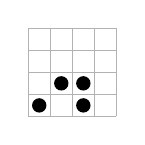
\begin{tikzpicture}[scale=0.28]
\draw[step=1,black!30] (0,0) grid (4,4);
\filldraw[black] (1.5,1.5) circle (0.30);
\filldraw[black] (2.5,1.5) circle (0.30);
\filldraw[black] (0.5,0.5) circle (0.30);
\filldraw[black] (2.5,0.5) circle (0.30);

\end{tikzpicture}\\[-1pt]{\tiny\#22}\end{minipage}\hfill\begin{minipage}{2.0cm}\centering 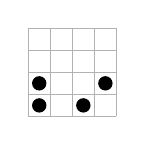
\begin{tikzpicture}[scale=0.28]
\draw[step=1,black!30] (0,0) grid (4,4);
\filldraw[black] (0.5,1.5) circle (0.30);
\filldraw[black] (3.5,1.5) circle (0.30);
\filldraw[black] (0.5,0.5) circle (0.30);
\filldraw[black] (2.5,0.5) circle (0.30);

\end{tikzpicture}\\[-1pt]{\tiny\#23}\end{minipage}\hfill\begin{minipage}{2.0cm}\centering 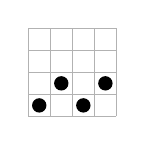
\begin{tikzpicture}[scale=0.28]
\draw[step=1,black!30] (0,0) grid (4,4);
\filldraw[black] (1.5,1.5) circle (0.30);
\filldraw[black] (3.5,1.5) circle (0.30);
\filldraw[black] (0.5,0.5) circle (0.30);
\filldraw[black] (2.5,0.5) circle (0.30);

\end{tikzpicture}\\[-1pt]{\tiny\#24}\end{minipage}}\par\vspace{6pt}
\noindent\makebox[\textwidth]{\begin{minipage}{2.0cm}\centering 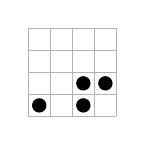
\begin{tikzpicture}[scale=0.28]
\draw[step=1,black!30] (0,0) grid (4,4);
\filldraw[black] (2.5,1.5) circle (0.30);
\filldraw[black] (3.5,1.5) circle (0.30);
\filldraw[black] (0.5,0.5) circle (0.30);
\filldraw[black] (2.5,0.5) circle (0.30);

\end{tikzpicture}\\[-1pt]{\tiny\#25}\end{minipage}\hfill\begin{minipage}{2.0cm}\centering 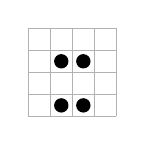
\begin{tikzpicture}[scale=0.28]
\draw[step=1,black!30] (0,0) grid (4,4);
\filldraw[black] (1.5,2.5) circle (0.30);
\filldraw[black] (2.5,2.5) circle (0.30);
\filldraw[black] (1.5,0.5) circle (0.30);
\filldraw[black] (2.5,0.5) circle (0.30);

\end{tikzpicture}\\[-1pt]{\tiny\#26}\end{minipage}\hfill\begin{minipage}{2.0cm}\centering 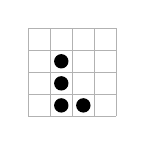
\begin{tikzpicture}[scale=0.28]
\draw[step=1,black!30] (0,0) grid (4,4);
\filldraw[black] (1.5,2.5) circle (0.30);
\filldraw[black] (1.5,1.5) circle (0.30);
\filldraw[black] (1.5,0.5) circle (0.30);
\filldraw[black] (2.5,0.5) circle (0.30);

\end{tikzpicture}\\[-1pt]{\tiny\#27}\end{minipage}\hfill\begin{minipage}{2.0cm}\centering 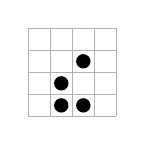
\begin{tikzpicture}[scale=0.28]
\draw[step=1,black!30] (0,0) grid (4,4);
\filldraw[black] (2.5,2.5) circle (0.30);
\filldraw[black] (1.5,1.5) circle (0.30);
\filldraw[black] (1.5,0.5) circle (0.30);
\filldraw[black] (2.5,0.5) circle (0.30);

\end{tikzpicture}\\[-1pt]{\tiny\#28}\end{minipage}\hfill\begin{minipage}{2.0cm}\centering 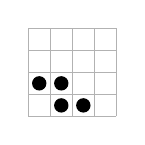
\begin{tikzpicture}[scale=0.28]
\draw[step=1,black!30] (0,0) grid (4,4);
\filldraw[black] (0.5,1.5) circle (0.30);
\filldraw[black] (1.5,1.5) circle (0.30);
\filldraw[black] (1.5,0.5) circle (0.30);
\filldraw[black] (2.5,0.5) circle (0.30);

\end{tikzpicture}\\[-1pt]{\tiny\#29}\end{minipage}\hfill\begin{minipage}{2.0cm}\centering 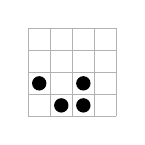
\begin{tikzpicture}[scale=0.28]
\draw[step=1,black!30] (0,0) grid (4,4);
\filldraw[black] (0.5,1.5) circle (0.30);
\filldraw[black] (2.5,1.5) circle (0.30);
\filldraw[black] (1.5,0.5) circle (0.30);
\filldraw[black] (2.5,0.5) circle (0.30);

\end{tikzpicture}\\[-1pt]{\tiny\#30}\end{minipage}}\par\vspace{6pt}
\noindent\makebox[\textwidth]{\begin{minipage}{2.0cm}\centering 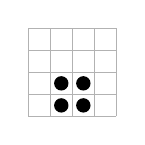
\begin{tikzpicture}[scale=0.28]
\draw[step=1,black!30] (0,0) grid (4,4);
\filldraw[black] (1.5,1.5) circle (0.30);
\filldraw[black] (2.5,1.5) circle (0.30);
\filldraw[black] (1.5,0.5) circle (0.30);
\filldraw[black] (2.5,0.5) circle (0.30);

\end{tikzpicture}\\[-1pt]{\tiny\#31}\end{minipage}\hfill\begin{minipage}{2.0cm}\centering 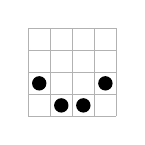
\begin{tikzpicture}[scale=0.28]
\draw[step=1,black!30] (0,0) grid (4,4);
\filldraw[black] (0.5,1.5) circle (0.30);
\filldraw[black] (3.5,1.5) circle (0.30);
\filldraw[black] (1.5,0.5) circle (0.30);
\filldraw[black] (2.5,0.5) circle (0.30);

\end{tikzpicture}\\[-1pt]{\tiny\#32}\end{minipage}\hfill\begin{minipage}{2.0cm}\centering 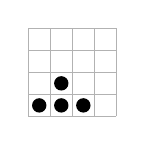
\begin{tikzpicture}[scale=0.28]
\draw[step=1,black!30] (0,0) grid (4,4);
\filldraw[black] (1.5,1.5) circle (0.30);
\filldraw[black] (0.5,0.5) circle (0.30);
\filldraw[black] (1.5,0.5) circle (0.30);
\filldraw[black] (2.5,0.5) circle (0.30);

\end{tikzpicture}\\[-1pt]{\tiny\#33}\end{minipage}\hfill\begin{minipage}{2.0cm}\centering 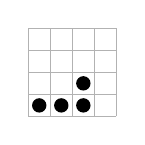
\begin{tikzpicture}[scale=0.28]
\draw[step=1,black!30] (0,0) grid (4,4);
\filldraw[black] (2.5,1.5) circle (0.30);
\filldraw[black] (0.5,0.5) circle (0.30);
\filldraw[black] (1.5,0.5) circle (0.30);
\filldraw[black] (2.5,0.5) circle (0.30);

\end{tikzpicture}\\[-1pt]{\tiny\#34}\end{minipage}\hfill\begin{minipage}{2.0cm}\centering 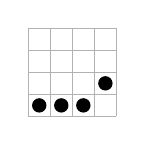
\begin{tikzpicture}[scale=0.28]
\draw[step=1,black!30] (0,0) grid (4,4);
\filldraw[black] (3.5,1.5) circle (0.30);
\filldraw[black] (0.5,0.5) circle (0.30);
\filldraw[black] (1.5,0.5) circle (0.30);
\filldraw[black] (2.5,0.5) circle (0.30);

\end{tikzpicture}\\[-1pt]{\tiny\#35}\end{minipage}\hfill\begin{minipage}{2.0cm}\centering 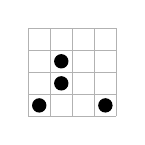
\begin{tikzpicture}[scale=0.28]
\draw[step=1,black!30] (0,0) grid (4,4);
\filldraw[black] (1.5,2.5) circle (0.30);
\filldraw[black] (1.5,1.5) circle (0.30);
\filldraw[black] (0.5,0.5) circle (0.30);
\filldraw[black] (3.5,0.5) circle (0.30);

\end{tikzpicture}\\[-1pt]{\tiny\#36}\end{minipage}}\par\vspace{6pt}
\noindent\makebox[\textwidth]{\begin{minipage}{2.0cm}\centering 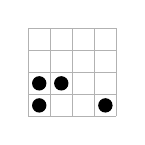
\begin{tikzpicture}[scale=0.28]
\draw[step=1,black!30] (0,0) grid (4,4);
\filldraw[black] (0.5,1.5) circle (0.30);
\filldraw[black] (1.5,1.5) circle (0.30);
\filldraw[black] (0.5,0.5) circle (0.30);
\filldraw[black] (3.5,0.5) circle (0.30);

\end{tikzpicture}\\[-1pt]{\tiny\#37}\end{minipage}\hfill\begin{minipage}{2.0cm}\centering 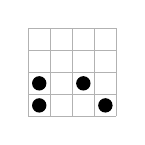
\begin{tikzpicture}[scale=0.28]
\draw[step=1,black!30] (0,0) grid (4,4);
\filldraw[black] (0.5,1.5) circle (0.30);
\filldraw[black] (2.5,1.5) circle (0.30);
\filldraw[black] (0.5,0.5) circle (0.30);
\filldraw[black] (3.5,0.5) circle (0.30);

\end{tikzpicture}\\[-1pt]{\tiny\#38}\end{minipage}\hfill\begin{minipage}{2.0cm}\centering 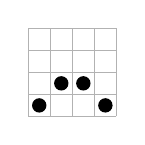
\begin{tikzpicture}[scale=0.28]
\draw[step=1,black!30] (0,0) grid (4,4);
\filldraw[black] (1.5,1.5) circle (0.30);
\filldraw[black] (2.5,1.5) circle (0.30);
\filldraw[black] (0.5,0.5) circle (0.30);
\filldraw[black] (3.5,0.5) circle (0.30);

\end{tikzpicture}\\[-1pt]{\tiny\#39}\end{minipage}\hfill\begin{minipage}{2.0cm}\centering 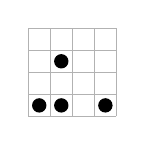
\begin{tikzpicture}[scale=0.28]
\draw[step=1,black!30] (0,0) grid (4,4);
\filldraw[black] (1.5,2.5) circle (0.30);
\filldraw[black] (0.5,0.5) circle (0.30);
\filldraw[black] (1.5,0.5) circle (0.30);
\filldraw[black] (3.5,0.5) circle (0.30);

\end{tikzpicture}\\[-1pt]{\tiny\#40}\end{minipage}\hfill\begin{minipage}{2.0cm}\centering 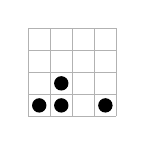
\begin{tikzpicture}[scale=0.28]
\draw[step=1,black!30] (0,0) grid (4,4);
\filldraw[black] (1.5,1.5) circle (0.30);
\filldraw[black] (0.5,0.5) circle (0.30);
\filldraw[black] (1.5,0.5) circle (0.30);
\filldraw[black] (3.5,0.5) circle (0.30);

\end{tikzpicture}\\[-1pt]{\tiny\#41}\end{minipage}\hfill\begin{minipage}{2.0cm}\centering 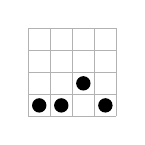
\begin{tikzpicture}[scale=0.28]
\draw[step=1,black!30] (0,0) grid (4,4);
\filldraw[black] (2.5,1.5) circle (0.30);
\filldraw[black] (0.5,0.5) circle (0.30);
\filldraw[black] (1.5,0.5) circle (0.30);
\filldraw[black] (3.5,0.5) circle (0.30);

\end{tikzpicture}\\[-1pt]{\tiny\#42}\end{minipage}}\par\vspace{6pt}
\noindent\makebox[\textwidth]{\begin{minipage}{2.0cm}\centering 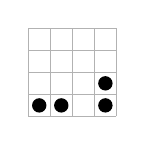
\begin{tikzpicture}[scale=0.28]
\draw[step=1,black!30] (0,0) grid (4,4);
\filldraw[black] (3.5,1.5) circle (0.30);
\filldraw[black] (0.5,0.5) circle (0.30);
\filldraw[black] (1.5,0.5) circle (0.30);
\filldraw[black] (3.5,0.5) circle (0.30);

\end{tikzpicture}\\[-1pt]{\tiny\#43}\end{minipage}\hfill\begin{minipage}{2.0cm}\centering 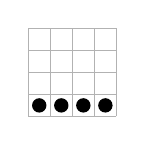
\begin{tikzpicture}[scale=0.28]
\draw[step=1,black!30] (0,0) grid (4,4);
\filldraw[black] (0.5,0.5) circle (0.30);
\filldraw[black] (1.5,0.5) circle (0.30);
\filldraw[black] (2.5,0.5) circle (0.30);
\filldraw[black] (3.5,0.5) circle (0.30);

\end{tikzpicture}\\[-1pt]{\tiny\#44}\end{minipage}\hfill\begin{minipage}{2.0cm}\centering 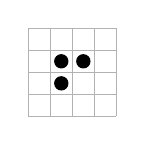
\begin{tikzpicture}[scale=0.28]
\draw[step=1,black!30] (0,0) grid (4,4);
\filldraw[black] (1.5,2.5) circle (0.30);
\filldraw[black] (2.5,2.5) circle (0.30);
\filldraw[black] (1.5,1.5) circle (0.30);

\end{tikzpicture}\\[-1pt]{\tiny\#45}\end{minipage}\hfill\begin{minipage}{2.0cm}\centering \begin{tikzpicture}[scale=0.28]
\draw[step=1,black!30] (0,0) grid (4,4);
\filldraw[black] (2.5,2.5) circle (0.30);
\filldraw[black] (0.5,1.5) circle (0.30);
\filldraw[black] (1.5,1.5) circle (0.30);

\end{tikzpicture}\\[-1pt]{\tiny\#46}\end{minipage}\hfill\begin{minipage}{2.0cm}\centering \begin{tikzpicture}[scale=0.28]
\draw[step=1,black!30] (0,0) grid (4,4);
\filldraw[black] (1.5,2.5) circle (0.30);
\filldraw[black] (1.5,1.5) circle (0.30);
\filldraw[black] (2.5,1.5) circle (0.30);

\end{tikzpicture}\\[-1pt]{\tiny\#47}\end{minipage}\hfill\begin{minipage}{2.0cm}\centering \begin{tikzpicture}[scale=0.28]
\draw[step=1,black!30] (0,0) grid (4,4);
\filldraw[black] (1.5,2.5) circle (0.30);
\filldraw[black] (0.5,1.5) circle (0.30);
\filldraw[black] (0.5,0.5) circle (0.30);

\end{tikzpicture}\\[-1pt]{\tiny\#48}\end{minipage}}\par\vspace{6pt}
\noindent\makebox[\textwidth]{\begin{minipage}{2.0cm}\centering \begin{tikzpicture}[scale=0.28]
\draw[step=1,black!30] (0,0) grid (4,4);
\filldraw[black] (1.5,2.5) circle (0.30);
\filldraw[black] (1.5,1.5) circle (0.30);
\filldraw[black] (0.5,0.5) circle (0.30);

\end{tikzpicture}\\[-1pt]{\tiny\#49}\end{minipage}\hfill\begin{minipage}{2.0cm}\centering \begin{tikzpicture}[scale=0.28]
\draw[step=1,black!30] (0,0) grid (4,4);
\filldraw[black] (2.5,2.5) circle (0.30);
\filldraw[black] (1.5,1.5) circle (0.30);
\filldraw[black] (0.5,0.5) circle (0.30);

\end{tikzpicture}\\[-1pt]{\tiny\#50}\end{minipage}\hfill\begin{minipage}{2.0cm}\centering \begin{tikzpicture}[scale=0.28]
\draw[step=1,black!30] (0,0) grid (4,4);
\filldraw[black] (2.5,2.5) circle (0.30);
\filldraw[black] (2.5,1.5) circle (0.30);
\filldraw[black] (0.5,0.5) circle (0.30);

\end{tikzpicture}\\[-1pt]{\tiny\#51}\end{minipage}\hfill\begin{minipage}{2.0cm}\centering \begin{tikzpicture}[scale=0.28]
\draw[step=1,black!30] (0,0) grid (4,4);
\filldraw[black] (1.5,1.5) circle (0.30);
\filldraw[black] (2.5,1.5) circle (0.30);
\filldraw[black] (0.5,0.5) circle (0.30);

\end{tikzpicture}\\[-1pt]{\tiny\#52}\end{minipage}\hfill\begin{minipage}{2.0cm}\centering \begin{tikzpicture}[scale=0.28]
\draw[step=1,black!30] (0,0) grid (4,4);
\filldraw[black] (2.5,1.5) circle (0.30);
\filldraw[black] (3.5,1.5) circle (0.30);
\filldraw[black] (0.5,0.5) circle (0.30);

\end{tikzpicture}\\[-1pt]{\tiny\#53}\end{minipage}\hfill\begin{minipage}{2.0cm}\centering \begin{tikzpicture}[scale=0.28]
\draw[step=1,black!30] (0,0) grid (4,4);
\filldraw[black] (1.5,2.5) circle (0.30);
\filldraw[black] (2.5,2.5) circle (0.30);
\filldraw[black] (1.5,0.5) circle (0.30);

\end{tikzpicture}\\[-1pt]{\tiny\#54}\end{minipage}}\par\vspace{6pt}
\noindent\makebox[\textwidth]{\begin{minipage}{2.0cm}\centering \begin{tikzpicture}[scale=0.28]
\draw[step=1,black!30] (0,0) grid (4,4);
\filldraw[black] (1.5,2.5) circle (0.30);
\filldraw[black] (0.5,1.5) circle (0.30);
\filldraw[black] (1.5,0.5) circle (0.30);

\end{tikzpicture}\\[-1pt]{\tiny\#55}\end{minipage}\hfill\begin{minipage}{2.0cm}\centering \begin{tikzpicture}[scale=0.28]
\draw[step=1,black!30] (0,0) grid (4,4);
\filldraw[black] (2.5,2.5) circle (0.30);
\filldraw[black] (0.5,1.5) circle (0.30);
\filldraw[black] (1.5,0.5) circle (0.30);

\end{tikzpicture}\\[-1pt]{\tiny\#56}\end{minipage}\hfill\begin{minipage}{2.0cm}\centering \begin{tikzpicture}[scale=0.28]
\draw[step=1,black!30] (0,0) grid (4,4);
\filldraw[black] (1.5,2.5) circle (0.30);
\filldraw[black] (1.5,1.5) circle (0.30);
\filldraw[black] (1.5,0.5) circle (0.30);

\end{tikzpicture}\\[-1pt]{\tiny\#57}\end{minipage}\hfill\begin{minipage}{2.0cm}\centering \begin{tikzpicture}[scale=0.28]
\draw[step=1,black!30] (0,0) grid (4,4);
\filldraw[black] (2.5,2.5) circle (0.30);
\filldraw[black] (1.5,1.5) circle (0.30);
\filldraw[black] (1.5,0.5) circle (0.30);

\end{tikzpicture}\\[-1pt]{\tiny\#58}\end{minipage}\hfill\begin{minipage}{2.0cm}\centering \begin{tikzpicture}[scale=0.28]
\draw[step=1,black!30] (0,0) grid (4,4);
\filldraw[black] (0.5,1.5) circle (0.30);
\filldraw[black] (1.5,1.5) circle (0.30);
\filldraw[black] (1.5,0.5) circle (0.30);

\end{tikzpicture}\\[-1pt]{\tiny\#59}\end{minipage}\hfill\begin{minipage}{2.0cm}\centering \begin{tikzpicture}[scale=0.28]
\draw[step=1,black!30] (0,0) grid (4,4);
\filldraw[black] (1.5,2.5) circle (0.30);
\filldraw[black] (2.5,1.5) circle (0.30);
\filldraw[black] (1.5,0.5) circle (0.30);

\end{tikzpicture}\\[-1pt]{\tiny\#60}\end{minipage}}\par\vspace{6pt}
\noindent\makebox[\textwidth]{\begin{minipage}{2.0cm}\centering \begin{tikzpicture}[scale=0.28]
\draw[step=1,black!30] (0,0) grid (4,4);
\filldraw[black] (2.5,2.5) circle (0.30);
\filldraw[black] (2.5,1.5) circle (0.30);
\filldraw[black] (1.5,0.5) circle (0.30);

\end{tikzpicture}\\[-1pt]{\tiny\#61}\end{minipage}\hfill\begin{minipage}{2.0cm}\centering \begin{tikzpicture}[scale=0.28]
\draw[step=1,black!30] (0,0) grid (4,4);
\filldraw[black] (0.5,1.5) circle (0.30);
\filldraw[black] (2.5,1.5) circle (0.30);
\filldraw[black] (1.5,0.5) circle (0.30);

\end{tikzpicture}\\[-1pt]{\tiny\#62}\end{minipage}\hfill\begin{minipage}{2.0cm}\centering \begin{tikzpicture}[scale=0.28]
\draw[step=1,black!30] (0,0) grid (4,4);
\filldraw[black] (1.5,1.5) circle (0.30);
\filldraw[black] (2.5,1.5) circle (0.30);
\filldraw[black] (1.5,0.5) circle (0.30);

\end{tikzpicture}\\[-1pt]{\tiny\#63}\end{minipage}\hfill\begin{minipage}{2.0cm}\centering \begin{tikzpicture}[scale=0.28]
\draw[step=1,black!30] (0,0) grid (4,4);
\filldraw[black] (0.5,1.5) circle (0.30);
\filldraw[black] (3.5,1.5) circle (0.30);
\filldraw[black] (1.5,0.5) circle (0.30);

\end{tikzpicture}\\[-1pt]{\tiny\#64}\end{minipage}\hfill\begin{minipage}{2.0cm}\centering \begin{tikzpicture}[scale=0.28]
\draw[step=1,black!30] (0,0) grid (4,4);
\filldraw[black] (1.5,1.5) circle (0.30);
\filldraw[black] (3.5,1.5) circle (0.30);
\filldraw[black] (1.5,0.5) circle (0.30);

\end{tikzpicture}\\[-1pt]{\tiny\#65}\end{minipage}\hfill\begin{minipage}{2.0cm}\centering \begin{tikzpicture}[scale=0.28]
\draw[step=1,black!30] (0,0) grid (4,4);
\filldraw[black] (2.5,1.5) circle (0.30);
\filldraw[black] (3.5,1.5) circle (0.30);
\filldraw[black] (1.5,0.5) circle (0.30);

\end{tikzpicture}\\[-1pt]{\tiny\#66}\end{minipage}}\par\vspace{6pt}
\noindent\makebox[\textwidth]{\begin{minipage}{2.0cm}\centering \begin{tikzpicture}[scale=0.28]
\draw[step=1,black!30] (0,0) grid (4,4);
\filldraw[black] (2.5,2.5) circle (0.30);
\filldraw[black] (0.5,0.5) circle (0.30);
\filldraw[black] (1.5,0.5) circle (0.30);

\end{tikzpicture}\\[-1pt]{\tiny\#67}\end{minipage}\hfill\begin{minipage}{2.0cm}\centering \begin{tikzpicture}[scale=0.28]
\draw[step=1,black!30] (0,0) grid (4,4);
\filldraw[black] (1.5,1.5) circle (0.30);
\filldraw[black] (0.5,0.5) circle (0.30);
\filldraw[black] (1.5,0.5) circle (0.30);

\end{tikzpicture}\\[-1pt]{\tiny\#68}\end{minipage}\hfill\begin{minipage}{2.0cm}\centering \begin{tikzpicture}[scale=0.28]
\draw[step=1,black!30] (0,0) grid (4,4);
\filldraw[black] (2.5,1.5) circle (0.30);
\filldraw[black] (0.5,0.5) circle (0.30);
\filldraw[black] (1.5,0.5) circle (0.30);

\end{tikzpicture}\\[-1pt]{\tiny\#69}\end{minipage}\hfill\begin{minipage}{2.0cm}\centering \begin{tikzpicture}[scale=0.28]
\draw[step=1,black!30] (0,0) grid (4,4);
\filldraw[black] (2.5,2.5) circle (0.30);
\filldraw[black] (0.5,0.5) circle (0.30);
\filldraw[black] (2.5,0.5) circle (0.30);

\end{tikzpicture}\\[-1pt]{\tiny\#70}\end{minipage}\hfill\begin{minipage}{2.0cm}\centering \begin{tikzpicture}[scale=0.28]
\draw[step=1,black!30] (0,0) grid (4,4);
\filldraw[black] (0.5,1.5) circle (0.30);
\filldraw[black] (0.5,0.5) circle (0.30);
\filldraw[black] (2.5,0.5) circle (0.30);

\end{tikzpicture}\\[-1pt]{\tiny\#71}\end{minipage}\hfill\begin{minipage}{2.0cm}\centering \begin{tikzpicture}[scale=0.28]
\draw[step=1,black!30] (0,0) grid (4,4);
\filldraw[black] (1.5,1.5) circle (0.30);
\filldraw[black] (0.5,0.5) circle (0.30);
\filldraw[black] (2.5,0.5) circle (0.30);

\end{tikzpicture}\\[-1pt]{\tiny\#72}\end{minipage}}\par\vspace{6pt}
\noindent\makebox[\textwidth]{\begin{minipage}{2.0cm}\centering \begin{tikzpicture}[scale=0.28]
\draw[step=1,black!30] (0,0) grid (4,4);
\filldraw[black] (2.5,1.5) circle (0.30);
\filldraw[black] (0.5,0.5) circle (0.30);
\filldraw[black] (2.5,0.5) circle (0.30);

\end{tikzpicture}\\[-1pt]{\tiny\#73}\end{minipage}\hfill\begin{minipage}{2.0cm}\centering \begin{tikzpicture}[scale=0.28]
\draw[step=1,black!30] (0,0) grid (4,4);
\filldraw[black] (3.5,1.5) circle (0.30);
\filldraw[black] (0.5,0.5) circle (0.30);
\filldraw[black] (2.5,0.5) circle (0.30);

\end{tikzpicture}\\[-1pt]{\tiny\#74}\end{minipage}\hfill\begin{minipage}{2.0cm}\centering \begin{tikzpicture}[scale=0.28]
\draw[step=1,black!30] (0,0) grid (4,4);
\filldraw[black] (1.5,2.5) circle (0.30);
\filldraw[black] (1.5,0.5) circle (0.30);
\filldraw[black] (2.5,0.5) circle (0.30);

\end{tikzpicture}\\[-1pt]{\tiny\#75}\end{minipage}\hfill\begin{minipage}{2.0cm}\centering \begin{tikzpicture}[scale=0.28]
\draw[step=1,black!30] (0,0) grid (4,4);
\filldraw[black] (0.5,1.5) circle (0.30);
\filldraw[black] (1.5,0.5) circle (0.30);
\filldraw[black] (2.5,0.5) circle (0.30);

\end{tikzpicture}\\[-1pt]{\tiny\#76}\end{minipage}\hfill\begin{minipage}{2.0cm}\centering \begin{tikzpicture}[scale=0.28]
\draw[step=1,black!30] (0,0) grid (4,4);
\filldraw[black] (1.5,1.5) circle (0.30);
\filldraw[black] (1.5,0.5) circle (0.30);
\filldraw[black] (2.5,0.5) circle (0.30);

\end{tikzpicture}\\[-1pt]{\tiny\#77}\end{minipage}\hfill\begin{minipage}{2.0cm}\centering \begin{tikzpicture}[scale=0.28]
\draw[step=1,black!30] (0,0) grid (4,4);
\filldraw[black] (0.5,1.5) circle (0.30);
\filldraw[black] (0.5,0.5) circle (0.30);
\filldraw[black] (3.5,0.5) circle (0.30);

\end{tikzpicture}\\[-1pt]{\tiny\#78}\end{minipage}}\par\vspace{6pt}
\noindent\makebox[\textwidth]{\begin{minipage}{2.0cm}\centering \begin{tikzpicture}[scale=0.28]
\draw[step=1,black!30] (0,0) grid (4,4);
\filldraw[black] (1.5,1.5) circle (0.30);
\filldraw[black] (0.5,0.5) circle (0.30);
\filldraw[black] (3.5,0.5) circle (0.30);

\end{tikzpicture}\\[-1pt]{\tiny\#79}\end{minipage}\hfill\begin{minipage}{2.0cm}\ \end{minipage}\hfill\begin{minipage}{2.0cm}\ \end{minipage}\hfill\begin{minipage}{2.0cm}\ \end{minipage}\hfill\begin{minipage}{2.0cm}\ \end{minipage}\hfill\begin{minipage}{2.0cm}\ \end{minipage}}\par\vspace{6pt}

\section{The rule book}\label{app:book}

The complete book $\Pi$: for each of the $\Nbookshapes$ shapes, the ordered list of items,
to be scanned top to bottom. Coordinates are $rc$ as in Section~\ref{sec:game};
``\textit{cand.}'' marks a candidate item, which fires when the move is legal and keeps a
shape of the catalogue (or wins); all other items are conditionals on the opponent's
placement. Black applies the book after mirroring the position into canonical form; White
applies it after the colour reversal $\rho$ of Section~\ref{sec:sym}.

\begin{multicols}{2}\raggedcolumns\small
\noindent\textbf{Entry 1} \; \begin{tikzpicture}[scale=0.24]
\draw[step=1,black!30] (0,0) grid (4,4);
\filldraw[black] (0.5,1.5) circle (0.30);
\filldraw[black] (1.5,1.5) circle (0.30);
\filldraw[black] (2.5,1.5) circle (0.30);
\filldraw[black] (0.5,0.5) circle (0.30);

\end{tikzpicture}
\nopagebreak\begin{enumerate}[topsep=1pt,itemsep=0pt,parsep=0pt,leftmargin=2.2em,label=\arabic*.]
\item if opp not on 13: $41\!\to\!42$
\item if opp on 13 and row 1 has >=2 opp: $33\!\to\!43$
\item $41\!\to\!42$ \hfill\textit{(cand.)}
\end{enumerate}\smallskip
\noindent\textbf{Entry 2} \; \begin{tikzpicture}[scale=0.24]
\draw[step=1,black!30] (0,0) grid (4,4);
\filldraw[black] (2.5,2.5) circle (0.30);
\filldraw[black] (2.5,1.5) circle (0.30);
\filldraw[black] (3.5,1.5) circle (0.30);
\filldraw[black] (0.5,0.5) circle (0.30);

\end{tikzpicture}
\nopagebreak\begin{enumerate}[topsep=1pt,itemsep=0pt,parsep=0pt,leftmargin=2.2em,label=\arabic*.]
\item $41\!\to\!42$ \hfill\textit{(cand.)}
\end{enumerate}\smallskip
\noindent\textbf{Entry 3} \; \begin{tikzpicture}[scale=0.24]
\draw[step=1,black!30] (0,0) grid (4,4);
\filldraw[black] (2.5,2.5) circle (0.30);
\filldraw[black] (0.5,1.5) circle (0.30);
\filldraw[black] (1.5,1.5) circle (0.30);
\filldraw[black] (1.5,0.5) circle (0.30);

\end{tikzpicture}
\nopagebreak\begin{enumerate}[topsep=1pt,itemsep=0pt,parsep=0pt,leftmargin=2.2em,label=\arabic*.]
\item if opp on 43 and opp not on 41: $31\!\to\!41$
\item if opp not on 13 and col 1 empty of opp: $42\!\to\!43$
\item if opp on 14 and opp not on 41: $31\!\to\!41$
\item if opp on 34 and row 4 empty of opp: $31\!\to\!41$
\item if opp on 21 and col 3 empty of opp: $23\!\to\!33$
\item if opp on 24 and opp not on 22: $42\!\to\!43$
\item if opp not on 41 and opp has no capturing move: $31\!\to\!41$
\item if opp not on 33 and opp not on 44: $23\!\to\!33$
\item if opp not on 12 and opp not on 22: $42\!\to\!43$
\item $31\!\to\!41$ \hfill\textit{(cand.)}
\item $42\!\to\!43$ \hfill\textit{(cand.)}
\end{enumerate}\smallskip
\noindent\textbf{Entry 4} \; \begin{tikzpicture}[scale=0.24]
\draw[step=1,black!30] (0,0) grid (4,4);
\filldraw[black] (0.5,1.5) circle (0.30);
\filldraw[black] (1.5,1.5) circle (0.30);
\filldraw[black] (2.5,1.5) circle (0.30);
\filldraw[black] (1.5,0.5) circle (0.30);

\end{tikzpicture}
\nopagebreak\begin{enumerate}[topsep=1pt,itemsep=0pt,parsep=0pt,leftmargin=2.2em,label=\arabic*.]
\item if opp not on 41 and col 3 has >=2 opp: $31\!\to\!41$
\item if opp on 44 and row 1 has >=2 opp: $33\!\to\!43$
\item if opp not on 22 and col 1 empty of opp: $31\!\to\!41$
\item if opp not on 43 and col 1 has >=2 opp: $33\!\to\!43$
\item if opp on 11 and row 1 has >=2 opp: $31\!\to\!41$
\item if opp on 21 and opp on 43: $31\!\to\!41$
\item if opp on 21 and opp on 44: $33\!\to\!43$
\item if opp on 21 and opp not on 12: $42\!\to\!41$
\item if opp not on 23 and col 2 empty of opp: $33\!\to\!23$
\item if col 3 empty of opp and row 4 has >=1 opp: $33\!\to\!43$
\item if row 4 empty of opp and opp has no capturing move: $31\!\to\!41$
\item if opp not on 43 and col 1 empty of opp: $33\!\to\!43$
\item if opp on 21 and opp not on 14: $42\!\to\!41$
\item if opp not on 41 and opp not on 44: $31\!\to\!41$
\item if opp not on 24 and opp not on 43: $33\!\to\!43$
\item $33\!\to\!23$ \hfill\textit{(cand.)}
\item $31\!\to\!41$ \hfill\textit{(cand.)}
\item $42\!\to\!43$ \hfill\textit{(cand.)}
\end{enumerate}\smallskip
\noindent\textbf{Entry 5} \; \begin{tikzpicture}[scale=0.24]
\draw[step=1,black!30] (0,0) grid (4,4);
\filldraw[black] (1.5,2.5) circle (0.30);
\filldraw[black] (2.5,1.5) circle (0.30);
\filldraw[black] (3.5,1.5) circle (0.30);
\filldraw[black] (1.5,0.5) circle (0.30);

\end{tikzpicture}
\nopagebreak\begin{enumerate}[topsep=1pt,itemsep=0pt,parsep=0pt,leftmargin=2.2em,label=\arabic*.]
\item if opp on 31 and opp not on 44: $34\!\to\!44$
\item if opp not on 13 and opp not on 43: $42\!\to\!43$
\item $22\!\to\!23$ \hfill\textit{(cand.)}
\item $34\!\to\!44$ \hfill\textit{(cand.)}
\end{enumerate}\smallskip
\noindent\textbf{Entry 6} \; \begin{tikzpicture}[scale=0.24]
\draw[step=1,black!30] (0,0) grid (4,4);
\filldraw[black] (2.5,2.5) circle (0.30);
\filldraw[black] (2.5,1.5) circle (0.30);
\filldraw[black] (3.5,1.5) circle (0.30);
\filldraw[black] (1.5,0.5) circle (0.30);

\end{tikzpicture}
\nopagebreak\begin{enumerate}[topsep=1pt,itemsep=0pt,parsep=0pt,leftmargin=2.2em,label=\arabic*.]
\item if opp not on 32 and opp not on 44: $34\!\to\!44$
\item if opp not on 13 and opp not on 22: $23\!\to\!22$
\item if opp not on 43 and row 4 has >=1 opp: $33\!\to\!43$
\item $34\!\to\!44$ \hfill\textit{(cand.)}
\end{enumerate}\smallskip
\noindent\textbf{Entry 7} \; \begin{tikzpicture}[scale=0.24]
\draw[step=1,black!30] (0,0) grid (4,4);
\filldraw[black] (1.5,2.5) circle (0.30);
\filldraw[black] (2.5,2.5) circle (0.30);
\filldraw[black] (0.5,0.5) circle (0.30);
\filldraw[black] (1.5,0.5) circle (0.30);

\end{tikzpicture}
\nopagebreak\begin{enumerate}[topsep=1pt,itemsep=0pt,parsep=0pt,leftmargin=2.2em,label=\arabic*.]
\item if opp not on 11 and opp not on 43: $42\!\to\!43$
\item if opp not on 24 and opp not on 33: $23\!\to\!33$
\item if opp not on 13 and opp not on 33: $23\!\to\!33$
\item if opp on 11 and opp not on 21: $42\!\to\!43$
\item $22\!\to\!32$ \hfill\textit{(cand.)}
\end{enumerate}\smallskip
\noindent\textbf{Entry 8} \; \begin{tikzpicture}[scale=0.24]
\draw[step=1,black!30] (0,0) grid (4,4);
\filldraw[black] (2.5,2.5) circle (0.30);
\filldraw[black] (1.5,1.5) circle (0.30);
\filldraw[black] (0.5,0.5) circle (0.30);
\filldraw[black] (1.5,0.5) circle (0.30);

\end{tikzpicture}
\nopagebreak\begin{enumerate}[topsep=1pt,itemsep=0pt,parsep=0pt,leftmargin=2.2em,label=\arabic*.]
\item if opp on 43 and opp not on 13: $32\!\to\!33$
\item if opp on 13 and col 4 has >=2 opp: $32\!\to\!33$
\item if row 2 empty of opp and row 4 empty of opp: $42\!\to\!43$
\item if col 1 empty of opp and col 3 empty of opp: $42\!\to\!43$
\item if row 1 empty of opp and opp has no capturing move: $42\!\to\!43$
\item if opp not on 12 and col 1 empty of opp: $41\!\to\!31$
\item if col 2 has >=2 opp and opp has no capturing move: $42\!\to\!43$
\item if opp on 34 and row 1 has >=2 opp: $23\!\to\!33$
\item if opp on 21 and col 4 empty of opp: $32\!\to\!22$
\item if opp on 33 and opp has no capturing move: $32\!\to\!22$
\item if opp on 33 and opp not on 31: $41\!\to\!31$
\item if opp on 34 and opp not on 31: $23\!\to\!33$
\item if col 2 empty of opp and row 4 empty of opp: $32\!\to\!22$
\item if col 4 has >=2 opp and row 1 has >=2 opp: $23\!\to\!33$
\item if opp not on 13 and col 2 empty of opp: $42\!\to\!43$
\item if opp not on 14 and row 2 empty of opp: $23\!\to\!33$
\item if opp on 12 and opp has a capturing move: $32\!\to\!22$
\item if opp on 11 and opp not on 13: $23\!\to\!33$
\item if opp not on 13 and opp not on 44: $42\!\to\!43$
\item if opp not on 31 and row 4 empty of opp: $32\!\to\!33$
\item if opp on 31: $23\!\to\!33$
\item if col 2 empty of opp and row 2 has >=1 opp: $32\!\to\!22$
\item if opp on 13 and opp on 14: $41\!\to\!31$
\item if opp on 11: $32\!\to\!33$
\item if opp on 12 and opp on 13: $32\!\to\!22$
\item $41\!\to\!31$ \hfill\textit{(cand.)}
\end{enumerate}\smallskip
\noindent\textbf{Entry 9} \; \begin{tikzpicture}[scale=0.24]
\draw[step=1,black!30] (0,0) grid (4,4);
\filldraw[black] (1.5,2.5) circle (0.30);
\filldraw[black] (2.5,1.5) circle (0.30);
\filldraw[black] (0.5,0.5) circle (0.30);
\filldraw[black] (1.5,0.5) circle (0.30);

\end{tikzpicture}
\nopagebreak\begin{enumerate}[topsep=1pt,itemsep=0pt,parsep=0pt,leftmargin=2.2em,label=\arabic*.]
\item if opp on 23 and opp not on 43: $42\!\to\!43$
\item if col 3 has >=1 opp and col 4 has >=2 opp: $22\!\to\!23$
\item if opp on 24 and opp not on 21: $33\!\to\!23$
\item if opp not on 43 and row 3 empty of opp: $42\!\to\!43$
\item if opp on 13 and row 4 empty of opp: $22\!\to\!23$
\item if opp not on 21 and row 4 empty of opp: $42\!\to\!43$
\item if opp on 34 and opp on 44: $42\!\to\!43$
\item if col 2 empty of opp and row 3 has >=1 opp: $22\!\to\!32$
\item if opp not on 21 and row 3 empty of opp: $22\!\to\!32$
\item if col 3 empty of opp and opp has no capturing move: $42\!\to\!43$
\item if opp on 21 and opp on 32: $33\!\to\!23$
\item if opp on 32 and opp not on 12: $22\!\to\!23$
\item $42\!\to\!43$ \hfill\textit{(cand.)}
\item if opp not on 13 and opp not on 23: $22\!\to\!23$
\item if opp on 13 and opp on 21: $33\!\to\!23$
\item $22\!\to\!32$ \hfill\textit{(cand.)}
\end{enumerate}\smallskip
\noindent\textbf{Entry 10} \; \begin{tikzpicture}[scale=0.24]
\draw[step=1,black!30] (0,0) grid (4,4);
\filldraw[black] (2.5,2.5) circle (0.30);
\filldraw[black] (2.5,1.5) circle (0.30);
\filldraw[black] (0.5,0.5) circle (0.30);
\filldraw[black] (1.5,0.5) circle (0.30);

\end{tikzpicture}
\nopagebreak\begin{enumerate}[topsep=1pt,itemsep=0pt,parsep=0pt,leftmargin=2.2em,label=\arabic*.]
\item if row 3 has >=1 opp and row 2 empty of opp: $23\!\to\!22$
\item if opp on 14 and row 3 empty of opp: $33\!\to\!32$
\item if opp on 22 and opp not on 44: $33\!\to\!32$
\item if opp not on 13 and row 4 empty of opp: $23\!\to\!22$
\item if opp on 11 and opp not on 12: $33\!\to\!32$
\item if opp on 44 and opp not on 43: $42\!\to\!43$
\item if opp on 43: $23\!\to\!22$
\item if opp not on 32 and opp has no capturing move: $33\!\to\!32$
\item if opp on 12: $23\!\to\!22$
\item $42\!\to\!43$ \hfill\textit{(cand.)}
\end{enumerate}\smallskip
\noindent\textbf{Entry 11} \; \begin{tikzpicture}[scale=0.24]
\draw[step=1,black!30] (0,0) grid (4,4);
\filldraw[black] (1.5,1.5) circle (0.30);
\filldraw[black] (2.5,1.5) circle (0.30);
\filldraw[black] (0.5,0.5) circle (0.30);
\filldraw[black] (1.5,0.5) circle (0.30);

\end{tikzpicture}
\nopagebreak\begin{enumerate}[topsep=1pt,itemsep=0pt,parsep=0pt,leftmargin=2.2em,label=\arabic*.]
\item if opp on 23 and opp not on 43: $42\!\to\!43$
\item if opp on 43 and row 3 empty of opp: $41\!\to\!31$
\item if col 2 empty of opp and col 3 empty of opp: $32\!\to\!22$
\item if col 1 empty of opp and row 4 empty of opp: $33\!\to\!23$
\item if opp not on 43 and col 1 empty of opp: $42\!\to\!43$
\item if col 2 empty of opp and row 1 has >=2 opp: $33\!\to\!23$
\item if opp on 43 and opp not on 23: $32\!\to\!22$
\item if opp on 31 and opp not on 34: $33\!\to\!34$
\item if opp not on 21 and row 2 empty of opp: $42\!\to\!43$
\item if opp on 22 and row 1 empty of opp: $42\!\to\!43$
\item if col 3 has >=1 opp and opp has no capturing move: $32\!\to\!22$
\item if opp on 12 and col 4 empty of opp: $42\!\to\!43$
\item if opp on 24 and opp on 34: $33\!\to\!23$
\item if opp not on 11 and opp not on 12: $42\!\to\!43$
\item if opp on 44 and opp not on 22: $32\!\to\!22$
\item if opp on 24 and col 4 has >=2 opp: $33\!\to\!23$
\item if opp on 22 and opp on 34: $33\!\to\!43$
\item if opp not on 13 and opp not on 21: $42\!\to\!43$
\item if opp on 22 and opp not on 21: $33\!\to\!43$
\item if opp on 11 and opp on 22: $33\!\to\!23$
\item if opp on 21 and opp on 24: $33\!\to\!43$
\item if opp not on 11 and opp not on 22: $41\!\to\!31$
\item if opp on 11 and opp on 21: $32\!\to\!22$
\item if opp on 12 and opp not on 44: $42\!\to\!43$
\item $41\!\to\!31$ \hfill\textit{(cand.)}
\end{enumerate}\smallskip
\noindent\textbf{Entry 12} \; \begin{tikzpicture}[scale=0.24]
\draw[step=1,black!30] (0,0) grid (4,4);
\filldraw[black] (0.5,1.5) circle (0.30);
\filldraw[black] (3.5,1.5) circle (0.30);
\filldraw[black] (0.5,0.5) circle (0.30);
\filldraw[black] (1.5,0.5) circle (0.30);

\end{tikzpicture}
\nopagebreak\begin{enumerate}[topsep=1pt,itemsep=0pt,parsep=0pt,leftmargin=2.2em,label=\arabic*.]
\item if opp not on 31 and row 3 empty of opp: $31\!\to\!32$
\item if opp on 33 and opp not on 44: $31\!\to\!32$
\item $42\!\to\!43$ \hfill\textit{(cand.)}
\end{enumerate}\smallskip
\noindent\textbf{Entry 13} \; \begin{tikzpicture}[scale=0.24]
\draw[step=1,black!30] (0,0) grid (4,4);
\filldraw[black] (1.5,1.5) circle (0.30);
\filldraw[black] (3.5,1.5) circle (0.30);
\filldraw[black] (0.5,0.5) circle (0.30);
\filldraw[black] (1.5,0.5) circle (0.30);

\end{tikzpicture}
\nopagebreak\begin{enumerate}[topsep=1pt,itemsep=0pt,parsep=0pt,leftmargin=2.2em,label=\arabic*.]
\item if opp on 31 and opp not on 33: $34\!\to\!33$
\item if opp on 21 and opp not on 11: $32\!\to\!31$
\item if opp not on 21 and col 4 empty of opp: $34\!\to\!44$
\item if opp not on 21 and col 3 empty of opp: $42\!\to\!43$
\item if opp on 23 and opp not on 43: $42\!\to\!43$
\item if opp on 43 and opp not on 44: $34\!\to\!44$
\item if opp on 11 and col 2 empty of opp: $42\!\to\!43$
\item if opp on 11 and opp not on 44: $34\!\to\!33$
\item if opp not on 33 and opp not on 43: $42\!\to\!43$
\item $34\!\to\!33$ \hfill\textit{(cand.)}
\item if opp not on 13 and row 2 empty of opp: $42\!\to\!43$
\item if opp not on 22 and opp not on 31: $32\!\to\!31$
\item $34\!\to\!44$ \hfill\textit{(cand.)}
\end{enumerate}\smallskip
\noindent\textbf{Entry 14} \; \begin{tikzpicture}[scale=0.24]
\draw[step=1,black!30] (0,0) grid (4,4);
\filldraw[black] (2.5,1.5) circle (0.30);
\filldraw[black] (3.5,1.5) circle (0.30);
\filldraw[black] (0.5,0.5) circle (0.30);
\filldraw[black] (1.5,0.5) circle (0.30);

\end{tikzpicture}
\nopagebreak\begin{enumerate}[topsep=1pt,itemsep=0pt,parsep=0pt,leftmargin=2.2em,label=\arabic*.]
\item if opp not on 44 and opp has no capturing move: $34\!\to\!44$
\item if opp not on 24 and opp has no capturing move: $33\!\to\!32$
\item if col 1 empty of opp and row 4 empty of opp: $42\!\to\!43$
\item if col 3 empty of opp and row 2 has >=1 opp: $33\!\to\!43$
\item if opp not on 12 and col 3 has >=2 opp: $34\!\to\!44$
\item if opp not on 22 and col 3 has >=1 opp: $42\!\to\!43$
\item if opp not on 23 and col 1 has >=1 opp: $33\!\to\!32$
\item $33\!\to\!43$ \hfill\textit{(cand.)}
\end{enumerate}\smallskip
\noindent\textbf{Entry 15} \; \begin{tikzpicture}[scale=0.24]
\draw[step=1,black!30] (0,0) grid (4,4);
\filldraw[black] (1.5,2.5) circle (0.30);
\filldraw[black] (2.5,2.5) circle (0.30);
\filldraw[black] (0.5,0.5) circle (0.30);
\filldraw[black] (2.5,0.5) circle (0.30);

\end{tikzpicture}
\nopagebreak\begin{enumerate}[topsep=1pt,itemsep=0pt,parsep=0pt,leftmargin=2.2em,label=\arabic*.]
\item if opp on 44 and opp not on 42: $41\!\to\!42$
\item if opp not on 22 and row 3 empty of opp: $23\!\to\!33$
\item if opp on 34 and col 3 empty of opp: $23\!\to\!33$
\item if opp not on 32 and row 2 empty of opp: $22\!\to\!32$
\item if opp not on 24 and row 1 has >=1 opp: $41\!\to\!42$
\item if opp not on 11 and col 2 empty of opp: $41\!\to\!42$
\item if opp on 32 and row 2 has >=1 opp: $41\!\to\!42$
\item if opp on 24 and opp not on 33: $22\!\to\!32$
\item if opp not on 21 and opp not on 34: $43\!\to\!42$
\item $22\!\to\!32$ \hfill\textit{(cand.)}
\end{enumerate}\smallskip
\noindent\textbf{Entry 16} \; \begin{tikzpicture}[scale=0.24]
\draw[step=1,black!30] (0,0) grid (4,4);
\filldraw[black] (1.5,2.5) circle (0.30);
\filldraw[black] (1.5,1.5) circle (0.30);
\filldraw[black] (0.5,0.5) circle (0.30);
\filldraw[black] (2.5,0.5) circle (0.30);

\end{tikzpicture}
\nopagebreak\begin{enumerate}[topsep=1pt,itemsep=0pt,parsep=0pt,leftmargin=2.2em,label=\arabic*.]
\item if row 3 empty of opp and opp has no capturing move: $32\!\to\!33$
\item if row 2 empty of opp and opp has no capturing move: $22\!\to\!23$
\item if opp on 23 and opp not on 33: $32\!\to\!33$
\item if opp on 24 and opp not on 33: $22\!\to\!23$
\item if opp not on 31 and opp not on 34: $41\!\to\!31$
\item if opp on 34 and opp not on 33: $32\!\to\!33$
\item $32\!\to\!31$ \hfill\textit{(cand.)}
\item if opp not on 23 and opp not on 44: $22\!\to\!23$
\item $41\!\to\!42$ \hfill\textit{(cand.)}
\end{enumerate}\smallskip
\noindent\textbf{Entry 17} \; \begin{tikzpicture}[scale=0.24]
\draw[step=1,black!30] (0,0) grid (4,4);
\filldraw[black] (2.5,2.5) circle (0.30);
\filldraw[black] (1.5,1.5) circle (0.30);
\filldraw[black] (0.5,0.5) circle (0.30);
\filldraw[black] (2.5,0.5) circle (0.30);

\end{tikzpicture}
\nopagebreak\begin{enumerate}[topsep=1pt,itemsep=0pt,parsep=0pt,leftmargin=2.2em,label=\arabic*.]
\item if col 2 empty of opp and row 3 empty of opp: $23\!\to\!33$
\item if row 2 empty of opp and row 3 empty of opp: $23\!\to\!22$
\item if opp on 44 and row 1 has >=2 opp: $41\!\to\!42$
\item if col 1 empty of opp and col 2 empty of opp: $32\!\to\!22$
\item if col 3 empty of opp and col 4 empty of opp: $23\!\to\!33$
\item if opp on 34 and col 2 has >=2 opp: $23\!\to\!33$
\item if col 3 empty of opp and row 2 empty of opp: $23\!\to\!22$
\item if opp on 31 and opp on 44: $41\!\to\!42$
\item if opp on 34 and row 2 has >=2 opp: $43\!\to\!42$
\item if opp on 21 and opp on 34: $32\!\to\!22$
\item if opp on 24 and opp on 34: $32\!\to\!22$
\item if row 1 has >=2 opp and row 2 has >=2 opp: $41\!\to\!42$
\item if opp on 24 and row 1 has >=2 opp: $32\!\to\!22$
\item if opp on 34 and opp has a capturing move: $41\!\to\!42$
\item if col 3 empty of opp and row 3 has >=1 opp: $23\!\to\!33$
\item if opp on 33 and col 2 has >=2 opp: $41\!\to\!31$
\item if opp on 21 and row 1 has >=2 opp: $32\!\to\!22$
\item if opp not on 22 and row 3 empty of opp: $23\!\to\!22$
\item if opp not on 31 and row 1 empty of opp: $41\!\to\!31$
\item if opp not on 33 and col 4 empty of opp: $23\!\to\!33$
\item if opp on 22 and opp not on 14: $41\!\to\!42$
\item if opp on 21 and opp not on 31: $41\!\to\!31$
\item if opp not on 14 and opp not on 33: $23\!\to\!22$
\item if col 1 empty of opp and row 4 has >=1 opp: $41\!\to\!31$
\item if opp not on 24 and col 1 empty of opp: $43\!\to\!42$
\item if opp not on 22 and row 2 has >=1 opp: $32\!\to\!22$
\item if opp not on 44 and col 2 empty of opp: $43\!\to\!42$
\item if opp on 31 and opp not on 22: $23\!\to\!22$
\item if opp not on 22 and opp not on 34: $41\!\to\!31$
\item $32\!\to\!22$ \hfill\textit{(cand.)}
\item if opp not on 12 and opp not on 24: $41\!\to\!42$
\item $23\!\to\!33$ \hfill\textit{(cand.)}
\item $41\!\to\!31$ \hfill\textit{(cand.)}
\end{enumerate}\smallskip
\noindent\textbf{Entry 18} \; \begin{tikzpicture}[scale=0.24]
\draw[step=1,black!30] (0,0) grid (4,4);
\filldraw[black] (0.5,1.5) circle (0.30);
\filldraw[black] (1.5,1.5) circle (0.30);
\filldraw[black] (0.5,0.5) circle (0.30);
\filldraw[black] (2.5,0.5) circle (0.30);

\end{tikzpicture}
\nopagebreak\begin{enumerate}[topsep=1pt,itemsep=0pt,parsep=0pt,leftmargin=2.2em,label=\arabic*.]
\item if opp not on 23: $41\!\to\!42$
\item $32\!\to\!33$ \hfill\textit{(cand.)}
\end{enumerate}\smallskip
\noindent\textbf{Entry 19} \; \begin{tikzpicture}[scale=0.24]
\draw[step=1,black!30] (0,0) grid (4,4);
\filldraw[black] (1.5,2.5) circle (0.30);
\filldraw[black] (2.5,1.5) circle (0.30);
\filldraw[black] (0.5,0.5) circle (0.30);
\filldraw[black] (2.5,0.5) circle (0.30);

\end{tikzpicture}
\nopagebreak\begin{enumerate}[topsep=1pt,itemsep=0pt,parsep=0pt,leftmargin=2.2em,label=\arabic*.]
\item if opp on 44 and col 2 empty of opp: $41\!\to\!42$
\item if opp on 44 and row 3 empty of opp: $33\!\to\!32$
\item if opp on 44 and opp not on 32: $22\!\to\!32$
\item if opp on 44 and opp has no capturing move: $41\!\to\!42$
\item if opp on 42 and col 4 empty of opp: $22\!\to\!32$
\item if opp not on 23 and row 1 empty of opp: $33\!\to\!23$
\item if opp on 34 and row 2 has >=2 opp: $22\!\to\!32$
\item if opp on 24 and opp on 34: $33\!\to\!23$
\item if col 2 empty of opp and col 3 empty of opp: $41\!\to\!42$
\item if opp on 12 and row 2 has >=2 opp: $33\!\to\!32$
\item if opp on 12 and opp on 21: $33\!\to\!23$
\item if opp on 12 and opp on 24: $33\!\to\!23$
\item if col 2 has >=1 opp and row 3 empty of opp: $33\!\to\!32$
\item if row 3 empty of opp and opp has no capturing move: $41\!\to\!42$
\item if opp not on 32 and row 2 has >=1 opp: $22\!\to\!32$
\item if opp on 14 and opp not on 32: $22\!\to\!32$
\item if opp not on 34 and row 2 empty of opp: $41\!\to\!42$
\item if opp not on 23 and row 2 has >=1 opp: $33\!\to\!23$
\item if opp not on 32 and opp has no capturing move: $33\!\to\!32$
\item if opp not on 42 and col 4 has >=1 opp: $43\!\to\!42$
\item $33\!\to\!32$ \hfill\textit{(cand.)}
\item if opp not on 11 and opp not on 31: $41\!\to\!42$
\item $43\!\to\!42$ \hfill\textit{(cand.)}
\end{enumerate}\smallskip
\noindent\textbf{Entry 20} \; \begin{tikzpicture}[scale=0.24]
\draw[step=1,black!30] (0,0) grid (4,4);
\filldraw[black] (2.5,2.5) circle (0.30);
\filldraw[black] (2.5,1.5) circle (0.30);
\filldraw[black] (0.5,0.5) circle (0.30);
\filldraw[black] (2.5,0.5) circle (0.30);

\end{tikzpicture}
\nopagebreak\begin{enumerate}[topsep=1pt,itemsep=0pt,parsep=0pt,leftmargin=2.2em,label=\arabic*.]
\item if opp not on 31 and col 2 empty of opp: $23\!\to\!22$
\item if opp not on 13 and row 2 empty of opp: $23\!\to\!22$
\item if opp on 14 and row 3 empty of opp: $33\!\to\!32$
\item if opp not on 32 and row 1 empty of opp: $33\!\to\!32$
\item if opp on 44 and opp not on 13: $41\!\to\!42$
\item if opp on 11 and row 4 empty of opp: $43\!\to\!42$
\item if opp on 22 and opp not on 12: $41\!\to\!42$
\item if opp not on 32 and col 1 empty of opp: $33\!\to\!32$
\item if opp on 12 and opp not on 31: $23\!\to\!22$
\item if opp on 13 and opp not on 44: $43\!\to\!42$
\item $33\!\to\!32$ \hfill\textit{(cand.)}
\item if opp on 32 and opp not on 21: $41\!\to\!42$
\item $23\!\to\!22$ \hfill\textit{(cand.)}
\end{enumerate}\smallskip
\noindent\textbf{Entry 21} \; \begin{tikzpicture}[scale=0.24]
\draw[step=1,black!30] (0,0) grid (4,4);
\filldraw[black] (0.5,1.5) circle (0.30);
\filldraw[black] (2.5,1.5) circle (0.30);
\filldraw[black] (0.5,0.5) circle (0.30);
\filldraw[black] (2.5,0.5) circle (0.30);

\end{tikzpicture}
\nopagebreak\begin{enumerate}[topsep=1pt,itemsep=0pt,parsep=0pt,leftmargin=2.2em,label=\arabic*.]
\item if opp on 34 and opp not on 32: $31\!\to\!32$
\item if opp not on 42 and col 4 has >=2 opp: $41\!\to\!42$
\item if opp not on 12 and col 2 empty of opp: $41\!\to\!42$
\item if opp not on 32 and opp not on 44: $31\!\to\!32$
\item $43\!\to\!44$ \hfill\textit{(cand.)}
\item if opp not on 22 and opp not on 23: $33\!\to\!34$
\item if opp not on 13 and opp not on 42: $41\!\to\!42$
\item if opp on 13 and opp not on 12: $41\!\to\!42$
\item if opp on 22: $31\!\to\!32$
\item $41\!\to\!42$ \hfill\textit{(cand.)}
\item $31\!\to\!32$ \hfill\textit{(cand.)}
\end{enumerate}\smallskip
\noindent\textbf{Entry 22} \; \begin{tikzpicture}[scale=0.24]
\draw[step=1,black!30] (0,0) grid (4,4);
\filldraw[black] (1.5,1.5) circle (0.30);
\filldraw[black] (2.5,1.5) circle (0.30);
\filldraw[black] (0.5,0.5) circle (0.30);
\filldraw[black] (2.5,0.5) circle (0.30);

\end{tikzpicture}
\nopagebreak\begin{enumerate}[topsep=1pt,itemsep=0pt,parsep=0pt,leftmargin=2.2em,label=\arabic*.]
\item if opp on 44 and opp not on 42: $41\!\to\!42$
\item if opp not on 31 and row 2 empty of opp: $32\!\to\!22$
\item if opp not on 42 and row 1 empty of opp: $43\!\to\!42$
\item if opp not on 34 and row 2 empty of opp: $33\!\to\!34$
\item if opp not on 44 and row 1 empty of opp: $43\!\to\!44$
\item if opp on 42 and col 2 has >=2 opp: $33\!\to\!34$
\item if opp on 22 and opp not on 12: $41\!\to\!42$
\item if opp not on 23 and col 1 empty of opp: $33\!\to\!23$
\item if opp on 34 and row 2 has >=2 opp: $32\!\to\!31$
\item if col 2 empty of opp and row 2 has >=2 opp: $32\!\to\!22$
\item if opp on 21 and opp has a capturing move: $32\!\to\!22$
\item if col 2 empty of opp and row 3 empty of opp: $32\!\to\!42$
\item if opp not on 31 and col 2 empty of opp: $32\!\to\!31$
\item if col 1 empty of opp and opp has a capturing move: $32\!\to\!42$
\item if opp not on 23 and col 4 empty of opp: $33\!\to\!34$
\item if opp not on 14 and col 2 empty of opp: $41\!\to\!42$
\item if col 4 empty of opp and row 1 has >=2 opp: $41\!\to\!42$
\item if opp not on 44 and col 1 empty of opp: $33\!\to\!34$
\item if opp on 42 and opp not on 11: $32\!\to\!31$
\item if col 2 has >=1 opp and col 4 has >=2 opp: $33\!\to\!23$
\item if opp not on 34 and col 3 empty of opp: $33\!\to\!34$
\item if opp on 23 and opp has no capturing move: $43\!\to\!44$
\item if opp not on 11 and opp not on 13: $43\!\to\!42$
\item if opp on 23 and opp not on 24: $32\!\to\!42$
\item if opp not on 13 and opp not on 22: $32\!\to\!22$
\item if opp on 11 and opp on 13: $33\!\to\!23$
\item $33\!\to\!34$ \hfill\textit{(cand.)}
\item if opp on 12: $43\!\to\!44$
\item $43\!\to\!42$ \hfill\textit{(cand.)}
\end{enumerate}\smallskip
\noindent\textbf{Entry 23} \; \begin{tikzpicture}[scale=0.24]
\draw[step=1,black!30] (0,0) grid (4,4);
\filldraw[black] (0.5,1.5) circle (0.30);
\filldraw[black] (3.5,1.5) circle (0.30);
\filldraw[black] (0.5,0.5) circle (0.30);
\filldraw[black] (2.5,0.5) circle (0.30);

\end{tikzpicture}
\nopagebreak\begin{enumerate}[topsep=1pt,itemsep=0pt,parsep=0pt,leftmargin=2.2em,label=\arabic*.]
\item if opp on 11 and opp not on 42: $41\!\to\!42$
\item if opp on 23 and opp not on 13: $34\!\to\!33$
\item if opp on 44 and opp not on 42: $41\!\to\!42$
\item if opp not on 21 and row 3 empty of opp: $31\!\to\!32$
\item if opp on 21 and opp not on 33: $34\!\to\!33$
\item if opp on 33 and opp has a capturing move: $43\!\to\!42$
\item $31\!\to\!32$ \hfill\textit{(cand.)}
\item if opp on 32 and opp not on 14: $34\!\to\!33$
\item if opp on 14 and opp not on 12: $41\!\to\!42$
\item $34\!\to\!33$ \hfill\textit{(cand.)}
\end{enumerate}\smallskip
\noindent\textbf{Entry 24} \; \begin{tikzpicture}[scale=0.24]
\draw[step=1,black!30] (0,0) grid (4,4);
\filldraw[black] (1.5,1.5) circle (0.30);
\filldraw[black] (3.5,1.5) circle (0.30);
\filldraw[black] (0.5,0.5) circle (0.30);
\filldraw[black] (2.5,0.5) circle (0.30);

\end{tikzpicture}
\nopagebreak\begin{enumerate}[topsep=1pt,itemsep=0pt,parsep=0pt,leftmargin=2.2em,label=\arabic*.]
\item if opp not on 42 and col 3 empty of opp: $41\!\to\!42$
\item if opp not on 33 and col 2 empty of opp: $34\!\to\!33$
\item if opp on 31 and opp not on 33: $34\!\to\!33$
\item if opp on 42 and col 4 empty of opp: $34\!\to\!44$
\item if opp not on 44 and col 3 empty of opp: $34\!\to\!44$
\item if opp not on 13 and opp not on 33: $34\!\to\!33$
\item if opp on 44 and opp not on 13: $41\!\to\!42$
\item if opp on 24 and opp on 33: $43\!\to\!44$
\item if opp on 33 and opp has no capturing move: $34\!\to\!44$
\item if opp on 11 and opp on 22: $41\!\to\!42$
\item if opp not on 44 and opp has no capturing move: $34\!\to\!44$
\item if opp on 21 and opp not on 11: $32\!\to\!31$
\item if opp on 13 and opp has no capturing move: $34\!\to\!33$
\item if opp not on 12 and row 2 has >=2 opp: $41\!\to\!42$
\item if opp on 22 and opp not on 12: $43\!\to\!42$
\item if opp on 13 and opp on 24: $43\!\to\!44$
\item if opp on 13 and opp on 23: $32\!\to\!33$
\item if opp on 33 and row 1 has >=2 opp: $34\!\to\!44$
\item if opp on 33 and col 3 has >=2 opp: $43\!\to\!42$
\item if opp on 11: $41\!\to\!42$
\item $34\!\to\!44$ \hfill\textit{(cand.)}
\end{enumerate}\smallskip
\noindent\textbf{Entry 25} \; \begin{tikzpicture}[scale=0.24]
\draw[step=1,black!30] (0,0) grid (4,4);
\filldraw[black] (2.5,1.5) circle (0.30);
\filldraw[black] (3.5,1.5) circle (0.30);
\filldraw[black] (0.5,0.5) circle (0.30);
\filldraw[black] (2.5,0.5) circle (0.30);

\end{tikzpicture}
\nopagebreak\begin{enumerate}[topsep=1pt,itemsep=0pt,parsep=0pt,leftmargin=2.2em,label=\arabic*.]
\item if opp on 44 and opp not on 22: $41\!\to\!42$
\item if opp not on 32 and col 3 empty of opp: $33\!\to\!32$
\item if opp not on 31 and col 4 empty of opp: $34\!\to\!44$
\item if row 3 empty of opp and opp has no capturing move: $33\!\to\!32$
\item if opp on 14 and opp not on 11: $34\!\to\!44$
\item if opp on 24 and opp not on 11: $43\!\to\!44$
\item if opp on 31 and row 1 has >=1 opp: $41\!\to\!42$
\item if opp not on 13 and opp not on 22: $34\!\to\!44$
\item if opp on 23: $43\!\to\!42$
\item $34\!\to\!44$ \hfill\textit{(cand.)}
\end{enumerate}\smallskip
\noindent\textbf{Entry 26} \; \begin{tikzpicture}[scale=0.24]
\draw[step=1,black!30] (0,0) grid (4,4);
\filldraw[black] (1.5,2.5) circle (0.30);
\filldraw[black] (2.5,2.5) circle (0.30);
\filldraw[black] (1.5,0.5) circle (0.30);
\filldraw[black] (2.5,0.5) circle (0.30);

\end{tikzpicture}
\nopagebreak\begin{enumerate}[topsep=1pt,itemsep=0pt,parsep=0pt,leftmargin=2.2em,label=\arabic*.]
\item if opp not on 14 and opp not on 32: $22\!\to\!32$
\item if opp not on 31 and opp not on 41: $42\!\to\!41$
\item if opp on 14 and col 2 empty of opp: $22\!\to\!32$
\item if opp on 41 and opp not on 44: $43\!\to\!44$
\item $23\!\to\!33$ \hfill\textit{(cand.)}
\item $42\!\to\!41$ \hfill\textit{(cand.)}
\end{enumerate}\smallskip
\noindent\textbf{Entry 27} \; \begin{tikzpicture}[scale=0.24]
\draw[step=1,black!30] (0,0) grid (4,4);
\filldraw[black] (1.5,2.5) circle (0.30);
\filldraw[black] (1.5,1.5) circle (0.30);
\filldraw[black] (1.5,0.5) circle (0.30);
\filldraw[black] (2.5,0.5) circle (0.30);

\end{tikzpicture}
\nopagebreak\begin{enumerate}[topsep=1pt,itemsep=0pt,parsep=0pt,leftmargin=2.2em,label=\arabic*.]
\item if opp not on 12 and row 2 empty of opp: $22\!\to\!23$
\item if opp on 23 and col 4 has >=1 opp: $32\!\to\!33$
\item if opp on 24 and opp not on 12: $22\!\to\!23$
\item if opp on 14 and row 4 empty of opp: $42\!\to\!41$
\item if opp not on 13 and row 3 empty of opp: $32\!\to\!33$
\item if opp on 41 and opp not on 24: $43\!\to\!44$
\item if opp on 21 and opp not on 33: $32\!\to\!33$
\item if opp not on 11 and opp has no capturing move: $42\!\to\!41$
\item if opp not on 31 and opp has no capturing move: $42\!\to\!41$
\item if opp on 13 and opp not on 23: $22\!\to\!23$
\item if opp not on 33 and opp not on 44: $32\!\to\!33$
\item $43\!\to\!44$ \hfill\textit{(cand.)}
\item $42\!\to\!41$ \hfill\textit{(cand.)}
\end{enumerate}\smallskip
\noindent\textbf{Entry 28} \; \begin{tikzpicture}[scale=0.24]
\draw[step=1,black!30] (0,0) grid (4,4);
\filldraw[black] (2.5,2.5) circle (0.30);
\filldraw[black] (1.5,1.5) circle (0.30);
\filldraw[black] (1.5,0.5) circle (0.30);
\filldraw[black] (2.5,0.5) circle (0.30);

\end{tikzpicture}
\nopagebreak\begin{enumerate}[topsep=1pt,itemsep=0pt,parsep=0pt,leftmargin=2.2em,label=\arabic*.]
\item if opp not on 22 and opp has a capturing move: $32\!\to\!22$
\item if opp not on 22 and col 1 empty of opp: $42\!\to\!41$
\item if col 3 empty of opp and col 4 empty of opp: $23\!\to\!33$
\item if opp not on 13 and col 1 empty of opp: $42\!\to\!41$
\item if row 2 empty of opp and row 3 empty of opp: $32\!\to\!33$
\item if opp on 31 and row 2 has >=2 opp: $23\!\to\!33$
\item if opp on 24 and opp on 31: $32\!\to\!22$
\item if opp not on 41 and row 1 empty of opp: $42\!\to\!41$
\item if row 1 has >=2 opp and row 2 has >=2 opp: $43\!\to\!44$
\item if opp not on 22 and row 3 empty of opp: $32\!\to\!22$
\item if opp on 24 and opp on 34: $23\!\to\!33$
\item if opp on 44 and col 1 has >=2 opp: $23\!\to\!33$
\item if opp on 24 and opp not on 44: $43\!\to\!44$
\item if opp on 22 and col 1 has >=2 opp: $23\!\to\!33$
\item if opp on 11 and opp on 21: $32\!\to\!22$
\item if opp on 11 and opp on 31: $43\!\to\!44$
\item if col 2 has >=2 opp and row 4 empty of opp: $23\!\to\!33$
\item if opp on 12 and opp not on 41: $42\!\to\!41$
\item if col 3 empty of opp and row 2 empty of opp: $23\!\to\!33$
\item if opp on 13 and col 4 empty of opp: $43\!\to\!44$
\item if opp not on 22 and col 3 empty of opp: $32\!\to\!22$
\item if opp not on 22 and col 4 empty of opp: $23\!\to\!22$
\item if opp on 21 and opp not on 22: $32\!\to\!22$
\item if opp on 41 and opp not on 22: $43\!\to\!44$
\item if opp on 34 and row 4 has >=1 opp: $23\!\to\!33$
\item if opp on 33 and col 4 has >=1 opp: $42\!\to\!41$
\item if opp on 34 and opp not on 31: $23\!\to\!33$
\item if opp not on 44 and opp has no capturing move: $43\!\to\!44$
\item if opp not on 41 and col 3 empty of opp: $42\!\to\!41$
\item if opp on 44 and opp not on 14: $32\!\to\!33$
\item if opp on 13 and opp on 31: $23\!\to\!33$
\item $43\!\to\!44$ \hfill\textit{(cand.)}
\item $42\!\to\!41$ \hfill\textit{(cand.)}
\end{enumerate}\smallskip
\noindent\textbf{Entry 29} \; \begin{tikzpicture}[scale=0.24]
\draw[step=1,black!30] (0,0) grid (4,4);
\filldraw[black] (0.5,1.5) circle (0.30);
\filldraw[black] (1.5,1.5) circle (0.30);
\filldraw[black] (1.5,0.5) circle (0.30);
\filldraw[black] (2.5,0.5) circle (0.30);

\end{tikzpicture}
\nopagebreak\begin{enumerate}[topsep=1pt,itemsep=0pt,parsep=0pt,leftmargin=2.2em,label=\arabic*.]
\item if row 1 has >=2 opp and row 4 empty of opp: $31\!\to\!41$
\item if opp on 23 and col 4 has >=1 opp: $32\!\to\!33$
\item if opp on 21 and opp not on 41: $42\!\to\!41$
\item if col 3 empty of opp and row 1 has >=1 opp: $43\!\to\!33$
\item $31\!\to\!41$ \hfill\textit{(cand.)}
\item if opp not on 11 and opp not on 14: $32\!\to\!33$
\item $43\!\to\!44$ \hfill\textit{(cand.)}
\end{enumerate}\smallskip
\noindent\textbf{Entry 30} \; \begin{tikzpicture}[scale=0.24]
\draw[step=1,black!30] (0,0) grid (4,4);
\filldraw[black] (0.5,1.5) circle (0.30);
\filldraw[black] (2.5,1.5) circle (0.30);
\filldraw[black] (1.5,0.5) circle (0.30);
\filldraw[black] (2.5,0.5) circle (0.30);

\end{tikzpicture}
\nopagebreak\begin{enumerate}[topsep=1pt,itemsep=0pt,parsep=0pt,leftmargin=2.2em,label=\arabic*.]
\item if opp on 34 and opp not on 32: $31\!\to\!32$
\item if opp on 21 and opp has a capturing move: $42\!\to\!41$
\item if opp on 14 and opp on 22: $31\!\to\!32$
\item if opp not on 32 and row 2 empty of opp: $33\!\to\!34$
\item if col 2 empty of opp and col 3 empty of opp: $33\!\to\!34$
\item if opp on 22 and opp on 23: $31\!\to\!32$
\item if opp not on 44 and col 3 has >=2 opp: $43\!\to\!44$
\item if opp on 21 and opp on 22: $31\!\to\!32$
\item if opp on 14 and opp on 44: $42\!\to\!41$
\item if opp on 41 and col 4 empty of opp: $43\!\to\!44$
\item if opp on 13 and opp on 14: $33\!\to\!34$
\item if opp on 11 and opp on 14: $31\!\to\!41$
\item if col 4 has >=2 opp and col 2 empty of opp: $42\!\to\!41$
\item if opp not on 34 and row 1 empty of opp: $33\!\to\!34$
\item if opp on 22 and col 4 has >=1 opp: $33\!\to\!32$
\item if opp on 44 and opp not on 12: $42\!\to\!41$
\item if opp on 14 and col 1 has >=1 opp: $43\!\to\!44$
\item if opp not on 32 and col 3 empty of opp: $33\!\to\!34$
\item if opp on 32 and col 1 has >=1 opp: $43\!\to\!44$
\item if opp not on 22 and col 4 empty of opp: $31\!\to\!41$
\item if opp on 23 and col 1 has >=1 opp: $33\!\to\!34$
\item if opp on 12 and opp on 23: $31\!\to\!41$
\item if opp not on 11 and opp not on 32: $31\!\to\!32$
\item if opp on 14 and opp not on 24: $42\!\to\!41$
\item if opp not on 13 and opp not on 34: $33\!\to\!34$
\item if opp on 11 and opp on 22: $31\!\to\!32$
\item if opp on 11 and opp not on 41: $31\!\to\!41$
\item $33\!\to\!32$ \hfill\textit{(cand.)}
\item if col 3 has >=1 opp and row 2 has >=1 opp: $42\!\to\!41$
\item if opp on 32 and opp not on 12: $43\!\to\!44$
\item $42\!\to\!41$ \hfill\textit{(cand.)}
\end{enumerate}\smallskip
\noindent\textbf{Entry 31} \; \begin{tikzpicture}[scale=0.24]
\draw[step=1,black!30] (0,0) grid (4,4);
\filldraw[black] (1.5,1.5) circle (0.30);
\filldraw[black] (2.5,1.5) circle (0.30);
\filldraw[black] (1.5,0.5) circle (0.30);
\filldraw[black] (2.5,0.5) circle (0.30);

\end{tikzpicture}
\nopagebreak\begin{enumerate}[topsep=1pt,itemsep=0pt,parsep=0pt,leftmargin=2.2em,label=\arabic*.]
\item if opp not on 44 and row 2 empty of opp: $43\!\to\!44$
\item if opp not on 44 and row 1 empty of opp: $43\!\to\!44$
\item if col 3 empty of opp and row 1 has >=2 opp: $43\!\to\!44$
\item if opp not on 31 and col 3 empty of opp: $33\!\to\!23$
\item if col 3 empty of opp and col 4 empty of opp: $33\!\to\!34$
\item if opp on 21 and opp on 24: $33\!\to\!23$
\item if opp on 12 and opp on 24: $33\!\to\!34$
\item if opp on 24 and opp on 41: $33\!\to\!23$
\item if opp on 24 and opp not on 22: $33\!\to\!34$
\item if opp on 23 and row 3 has >=1 opp: $43\!\to\!44$
\item if opp not on 22 and opp not on 41: $32\!\to\!22$
\item if opp on 13 and opp not on 22: $43\!\to\!44$
\item if opp on 21 and opp not on 23: $33\!\to\!23$
\item if opp on 13 and opp not on 23: $33\!\to\!34$
\item if opp not on 12 and col 4 empty of opp: $43\!\to\!44$
\item if opp on 31 and opp on 44: $33\!\to\!23$
\item if opp on 41 and opp not on 21: $43\!\to\!44$
\item $32\!\to\!22$ \hfill\textit{(cand.)}
\item if opp on 23 and opp not on 11: $32\!\to\!31$
\item if opp on 14: $33\!\to\!23$
\item if opp on 11 and opp on 24: $33\!\to\!34$
\item $42\!\to\!41$ \hfill\textit{(cand.)}
\end{enumerate}\smallskip
\noindent\textbf{Entry 32} \; \begin{tikzpicture}[scale=0.24]
\draw[step=1,black!30] (0,0) grid (4,4);
\filldraw[black] (0.5,1.5) circle (0.30);
\filldraw[black] (3.5,1.5) circle (0.30);
\filldraw[black] (1.5,0.5) circle (0.30);
\filldraw[black] (2.5,0.5) circle (0.30);

\end{tikzpicture}
\nopagebreak\begin{enumerate}[topsep=1pt,itemsep=0pt,parsep=0pt,leftmargin=2.2em,label=\arabic*.]
\item if opp on 24 and opp not on 14: $43\!\to\!44$
\item if opp on 23 and opp not on 13: $34\!\to\!33$
\item if opp on 11 and opp not on 32: $31\!\to\!32$
\item if opp on 22 and opp not on 32: $31\!\to\!32$
\item if opp on 21 and opp not on 41: $42\!\to\!41$
\item if opp not on 32 and col 4 empty of opp: $43\!\to\!44$
\item if opp on 21 and opp not on 12: $34\!\to\!33$
\item if row 2 empty of opp and row 3 empty of opp: $34\!\to\!33$
\item if opp not on 23 and opp not on 32: $43\!\to\!44$
\item if opp not on 12 and col 4 has >=1 opp: $34\!\to\!33$
\item if opp on 11 and opp not on 41: $31\!\to\!41$
\item if opp on 32 and opp not on 12: $43\!\to\!44$
\item if opp not on 13 and opp not on 14: $34\!\to\!33$
\item if opp on 12 and opp on 13: $42\!\to\!41$
\item $31\!\to\!41$ \hfill\textit{(cand.)}
\end{enumerate}\smallskip
\noindent\textbf{Entry 33} \; \begin{tikzpicture}[scale=0.24]
\draw[step=1,black!30] (0,0) grid (4,4);
\filldraw[black] (1.5,1.5) circle (0.30);
\filldraw[black] (0.5,0.5) circle (0.30);
\filldraw[black] (1.5,0.5) circle (0.30);
\filldraw[black] (2.5,0.5) circle (0.30);

\end{tikzpicture}
\nopagebreak\begin{enumerate}[topsep=1pt,itemsep=0pt,parsep=0pt,leftmargin=2.2em,label=\arabic*.]
\item if col 3 empty of opp and row 3 has >=1 opp: $43\!\to\!33$
\item if col 2 empty of opp and row 3 empty of opp: $32\!\to\!33$
\item if opp not on 33 and col 2 empty of opp: $43\!\to\!33$
\item if opp on 33 and row 1 has >=2 opp: $41\!\to\!31$
\item if row 1 has >=2 opp and row 3 has >=1 opp: $43\!\to\!33$
\item if opp on 22 and col 4 empty of opp: $43\!\to\!44$
\item if opp not on 22 and col 3 empty of opp: $32\!\to\!33$
\item if opp on 33 and opp on 44: $41\!\to\!31$
\item if opp on 33 and row 3 has >=2 opp: $43\!\to\!44$
\item if opp on 33: $41\!\to\!31$
\item if opp not on 21 and opp not on 22: $32\!\to\!33$
\item if opp on 23 and col 1 empty of opp: $32\!\to\!33$
\item if opp not on 13 and col 1 empty of opp: $43\!\to\!33$
\item if opp on 14 and opp not on 44: $43\!\to\!44$
\item if opp not on 12 and opp not on 23: $41\!\to\!31$
\item if opp on 21 and opp not on 13: $32\!\to\!33$
\item if opp on 11 and col 3 has >=1 opp: $32\!\to\!33$
\item if opp on 12 and opp not on 44: $43\!\to\!44$
\item $41\!\to\!31$ \hfill\textit{(cand.)}
\item $43\!\to\!33$ \hfill\textit{(cand.)}
\end{enumerate}\smallskip
\noindent\textbf{Entry 34} \; \begin{tikzpicture}[scale=0.24]
\draw[step=1,black!30] (0,0) grid (4,4);
\filldraw[black] (2.5,1.5) circle (0.30);
\filldraw[black] (0.5,0.5) circle (0.30);
\filldraw[black] (1.5,0.5) circle (0.30);
\filldraw[black] (2.5,0.5) circle (0.30);

\end{tikzpicture}
\nopagebreak\begin{enumerate}[topsep=1pt,itemsep=0pt,parsep=0pt,leftmargin=2.2em,label=\arabic*.]
\item if opp not on 32 and row 3 has >=1 opp: $42\!\to\!32$
\item if opp on 44 and col 2 empty of opp: $42\!\to\!32$
\item if opp not on 12 and col 2 empty of opp: $41\!\to\!31$
\item if opp not on 12 and opp not on 32: $33\!\to\!32$
\item if opp not on 32 and row 2 empty of opp: $42\!\to\!32$
\item if opp on 32 and col 3 has >=1 opp: $43\!\to\!44$
\item if opp on 22 and col 1 has >=1 opp: $42\!\to\!32$
\item if opp not on 34 and row 2 empty of opp: $33\!\to\!34$
\item if opp on 11 and opp not on 24: $41\!\to\!31$
\item if opp on 23 and opp not on 13: $33\!\to\!32$
\item if opp on 24 and opp on 44: $33\!\to\!34$
\item if opp not on 12 and col 1 empty of opp: $41\!\to\!31$
\item if opp on 32 and opp not on 21: $43\!\to\!44$
\item if opp on 14 and opp on 21: $33\!\to\!34$
\item if opp on 22 and opp not on 14: $42\!\to\!32$
\item if opp on 14 and opp not on 22: $41\!\to\!31$
\item if opp on 21 and opp on 44: $33\!\to\!34$
\item if opp on 11 and opp not on 21: $42\!\to\!32$
\item if opp on 13 and opp not on 23: $33\!\to\!32$
\item if opp on 12 and opp not on 44: $43\!\to\!44$
\item if opp on 21 and opp on 24: $33\!\to\!34$
\item $43\!\to\!44$ \hfill\textit{(cand.)}
\item if opp on 12 and opp on 14: $42\!\to\!32$
\item $41\!\to\!31$ \hfill\textit{(cand.)}
\end{enumerate}\smallskip
\noindent\textbf{Entry 35} \; \begin{tikzpicture}[scale=0.24]
\draw[step=1,black!30] (0,0) grid (4,4);
\filldraw[black] (3.5,1.5) circle (0.30);
\filldraw[black] (0.5,0.5) circle (0.30);
\filldraw[black] (1.5,0.5) circle (0.30);
\filldraw[black] (2.5,0.5) circle (0.30);

\end{tikzpicture}
\nopagebreak\begin{enumerate}[topsep=1pt,itemsep=0pt,parsep=0pt,leftmargin=2.2em,label=\arabic*.]
\item if col 2 empty of opp and opp has no capturing move: $42\!\to\!32$
\item if opp on 32 and opp not on 31: $43\!\to\!33$
\item if opp on 22 and col 3 empty of opp: $42\!\to\!32$
\item if opp on 23: $34\!\to\!33$
\item if opp on 12 and row 2 empty of opp: $42\!\to\!32$
\item if opp not on 44 and opp has a capturing move: $43\!\to\!44$
\item if opp not on 21 and opp not on 32: $42\!\to\!32$
\item if opp on 21 and row 2 has >=2 opp: $41\!\to\!31$
\item if opp not on 13 and opp not on 24: $34\!\to\!33$
\item $42\!\to\!32$ \hfill\textit{(cand.)}
\item $43\!\to\!44$ \hfill\textit{(cand.)}
\end{enumerate}\smallskip
\noindent\textbf{Entry 36} \; \begin{tikzpicture}[scale=0.24]
\draw[step=1,black!30] (0,0) grid (4,4);
\filldraw[black] (1.5,2.5) circle (0.30);
\filldraw[black] (1.5,1.5) circle (0.30);
\filldraw[black] (0.5,0.5) circle (0.30);
\filldraw[black] (3.5,0.5) circle (0.30);

\end{tikzpicture}
\nopagebreak\begin{enumerate}[topsep=1pt,itemsep=0pt,parsep=0pt,leftmargin=2.2em,label=\arabic*.]
\item if opp not on 13 and opp not on 43: $44\!\to\!43$
\item if opp not on 12 and opp not on 33: $41\!\to\!42$
\item if opp on 13 and opp not on 21: $41\!\to\!42$
\item if opp on 13 and opp not on 23: $41\!\to\!31$
\item $32\!\to\!42$ \hfill\textit{(cand.)}
\end{enumerate}\smallskip
\noindent\textbf{Entry 37} \; \begin{tikzpicture}[scale=0.24]
\draw[step=1,black!30] (0,0) grid (4,4);
\filldraw[black] (0.5,1.5) circle (0.30);
\filldraw[black] (1.5,1.5) circle (0.30);
\filldraw[black] (0.5,0.5) circle (0.30);
\filldraw[black] (3.5,0.5) circle (0.30);

\end{tikzpicture}
\nopagebreak\begin{enumerate}[topsep=1pt,itemsep=0pt,parsep=0pt,leftmargin=2.2em,label=\arabic*.]
\item $41\!\to\!42$ \hfill\textit{(cand.)}
\end{enumerate}\smallskip
\noindent\textbf{Entry 38} \; \begin{tikzpicture}[scale=0.24]
\draw[step=1,black!30] (0,0) grid (4,4);
\filldraw[black] (0.5,1.5) circle (0.30);
\filldraw[black] (2.5,1.5) circle (0.30);
\filldraw[black] (0.5,0.5) circle (0.30);
\filldraw[black] (3.5,0.5) circle (0.30);

\end{tikzpicture}
\nopagebreak\begin{enumerate}[topsep=1pt,itemsep=0pt,parsep=0pt,leftmargin=2.2em,label=\arabic*.]
\item if opp not on 21 and opp not on 32: $31\!\to\!32$
\item if opp not on 11 and opp not on 42: $44\!\to\!43$
\item if opp on 21 and opp not on 12: $31\!\to\!32$
\item $41\!\to\!42$ \hfill\textit{(cand.)}
\end{enumerate}\smallskip
\noindent\textbf{Entry 39} \; \begin{tikzpicture}[scale=0.24]
\draw[step=1,black!30] (0,0) grid (4,4);
\filldraw[black] (1.5,1.5) circle (0.30);
\filldraw[black] (2.5,1.5) circle (0.30);
\filldraw[black] (0.5,0.5) circle (0.30);
\filldraw[black] (3.5,0.5) circle (0.30);

\end{tikzpicture}
\nopagebreak\begin{enumerate}[topsep=1pt,itemsep=0pt,parsep=0pt,leftmargin=2.2em,label=\arabic*.]
\item if col 2 has >=1 opp and opp has no capturing move: $33\!\to\!43$
\item if opp on 23 and opp not on 13: $44\!\to\!43$
\item if opp not on 13 and opp not on 42: $41\!\to\!42$
\item if opp on 42: $33\!\to\!43$
\item if opp on 22 and opp not on 12: $41\!\to\!42$
\item if opp not on 24 and opp has no capturing move: $32\!\to\!42$
\item if opp not on 22 and opp not on 24: $41\!\to\!42$
\item if opp on 13 and opp on 24: $33\!\to\!34$
\item if opp on 12 and opp not on 21: $44\!\to\!43$
\item $33\!\to\!43$ \hfill\textit{(cand.)}
\end{enumerate}\smallskip
\noindent\textbf{Entry 40} \; \begin{tikzpicture}[scale=0.24]
\draw[step=1,black!30] (0,0) grid (4,4);
\filldraw[black] (1.5,2.5) circle (0.30);
\filldraw[black] (0.5,0.5) circle (0.30);
\filldraw[black] (1.5,0.5) circle (0.30);
\filldraw[black] (3.5,0.5) circle (0.30);

\end{tikzpicture}
\nopagebreak\begin{enumerate}[topsep=1pt,itemsep=0pt,parsep=0pt,leftmargin=2.2em,label=\arabic*.]
\item if opp on 12: $42\!\to\!32$
\item if opp not on 12 and opp not on 24: $42\!\to\!32$
\item $22\!\to\!32$ \hfill\textit{(cand.)}
\end{enumerate}\smallskip
\noindent\textbf{Entry 41} \; \begin{tikzpicture}[scale=0.24]
\draw[step=1,black!30] (0,0) grid (4,4);
\filldraw[black] (1.5,1.5) circle (0.30);
\filldraw[black] (0.5,0.5) circle (0.30);
\filldraw[black] (1.5,0.5) circle (0.30);
\filldraw[black] (3.5,0.5) circle (0.30);

\end{tikzpicture}
\nopagebreak\begin{enumerate}[topsep=1pt,itemsep=0pt,parsep=0pt,leftmargin=2.2em,label=\arabic*.]
\item if opp on 43 and opp not on 33: $32\!\to\!33$
\item if col 3 empty of opp and row 3 empty of opp: $32\!\to\!33$
\item if opp not on 13 and col 3 empty of opp: $44\!\to\!43$
\item if col 2 empty of opp and row 3 empty of opp: $42\!\to\!43$
\item if opp on 33 and row 1 has >=2 opp: $41\!\to\!31$
\item if opp on 21 and row 3 has >=1 opp: $41\!\to\!31$
\item if opp not on 33 and row 2 empty of opp: $32\!\to\!33$
\item if opp not on 33 and col 3 has >=2 opp: $32\!\to\!33$
\item if opp not on 12 and row 3 empty of opp: $44\!\to\!43$
\item if col 1 empty of opp and col 4 empty of opp: $41\!\to\!31$
\item if opp on 31 and col 4 has >=1 opp: $42\!\to\!43$
\item if opp on 24 and opp on 33: $41\!\to\!31$
\item if opp not on 11 and col 2 has >=2 opp: $42\!\to\!43$
\item if opp on 21 and opp not on 11: $44\!\to\!43$
\item if opp on 33 and opp has a capturing move: $44\!\to\!43$
\item if opp not on 43 and col 3 has >=2 opp: $42\!\to\!43$
\item if opp on 23 and opp on 34: $32\!\to\!33$
\item if opp not on 14 and col 4 has >=1 opp: $44\!\to\!43$
\item if opp on 33 and opp not on 31: $41\!\to\!31$
\item if opp on 22 and opp on 23: $42\!\to\!43$
\item if opp on 23 and opp not on 11: $44\!\to\!34$
\item if opp on 12 and opp not on 11: $42\!\to\!43$
\item if opp on 12 and opp not on 22: $32\!\to\!22$
\item $41\!\to\!31$ \hfill\textit{(cand.)}
\item if opp on 31 and opp not on 11: $44\!\to\!34$
\item $32\!\to\!33$ \hfill\textit{(cand.)}
\end{enumerate}\smallskip
\noindent\textbf{Entry 42} \; \begin{tikzpicture}[scale=0.24]
\draw[step=1,black!30] (0,0) grid (4,4);
\filldraw[black] (2.5,1.5) circle (0.30);
\filldraw[black] (0.5,0.5) circle (0.30);
\filldraw[black] (1.5,0.5) circle (0.30);
\filldraw[black] (3.5,0.5) circle (0.30);

\end{tikzpicture}
\nopagebreak\begin{enumerate}[topsep=1pt,itemsep=0pt,parsep=0pt,leftmargin=2.2em,label=\arabic*.]
\item if opp not on 32 and row 3 has >=1 opp: $42\!\to\!32$
\item if col 2 empty of opp and opp has no capturing move: $41\!\to\!31$
\item if row 1 has >=2 opp and row 2 empty of opp: $44\!\to\!34$
\item if opp on 32 and col 3 has >=2 opp: $44\!\to\!34$
\item if opp on 23 and opp has a capturing move: $42\!\to\!43$
\item if opp on 23 and opp not on 12: $33\!\to\!32$
\item if opp on 13 and col 2 empty of opp: $44\!\to\!43$
\item if opp not on 12 and opp not on 32: $33\!\to\!32$
\item if opp not on 12 and col 4 empty of opp: $44\!\to\!34$
\item if opp on 21 and opp on 43: $44\!\to\!34$
\item if col 1 has >=1 opp and row 2 empty of opp: $42\!\to\!43$
\item if opp on 11 and opp on 32: $44\!\to\!34$
\item if opp on 24 and opp on 43: $33\!\to\!34$
\item if opp on 32 and row 2 has >=2 opp: $44\!\to\!34$
\item if opp on 11 and opp on 21: $44\!\to\!43$
\item if opp on 11 and opp not on 13: $42\!\to\!32$
\item if opp on 22 and opp has a capturing move: $42\!\to\!43$
\item if opp on 13 and opp on 24: $33\!\to\!34$
\item if opp not on 34 and opp has a capturing move: $44\!\to\!34$
\item if opp on 22 and row 1 has >=2 opp: $42\!\to\!32$
\item if col 1 empty of opp and opp has no capturing move: $41\!\to\!31$
\item if opp on 21 and opp not on 24: $42\!\to\!43$
\item if opp not on 14 and opp not on 32: $41\!\to\!31$
\item if opp on 14: $44\!\to\!43$
\item $33\!\to\!34$ \hfill\textit{(cand.)}
\item $42\!\to\!43$ \hfill\textit{(cand.)}
\end{enumerate}\smallskip
\noindent\textbf{Entry 43} \; \begin{tikzpicture}[scale=0.24]
\draw[step=1,black!30] (0,0) grid (4,4);
\filldraw[black] (3.5,1.5) circle (0.30);
\filldraw[black] (0.5,0.5) circle (0.30);
\filldraw[black] (1.5,0.5) circle (0.30);
\filldraw[black] (3.5,0.5) circle (0.30);

\end{tikzpicture}
\nopagebreak\begin{enumerate}[topsep=1pt,itemsep=0pt,parsep=0pt,leftmargin=2.2em,label=\arabic*.]
\item if opp not on 23 and row 3 empty of opp: $41\!\to\!31$
\item if opp on 33: $42\!\to\!32$
\item if opp not on 21 and row 3 has >=1 opp: $34\!\to\!33$
\item if opp not on 12 and opp not on 14: $34\!\to\!33$
\item if opp on 23 and opp not on 43: $41\!\to\!31$
\item $44\!\to\!43$ \hfill\textit{(cand.)}
\item $34\!\to\!33$ \hfill\textit{(cand.)}
\end{enumerate}\smallskip
\noindent\textbf{Entry 44} \; \begin{tikzpicture}[scale=0.24]
\draw[step=1,black!30] (0,0) grid (4,4);
\filldraw[black] (0.5,0.5) circle (0.30);
\filldraw[black] (1.5,0.5) circle (0.30);
\filldraw[black] (2.5,0.5) circle (0.30);
\filldraw[black] (3.5,0.5) circle (0.30);

\end{tikzpicture}
\nopagebreak\begin{enumerate}[topsep=1pt,itemsep=0pt,parsep=0pt,leftmargin=2.2em,label=\arabic*.]
\item if opp not on 23 and row 2 has >=1 opp: $44\!\to\!34$
\item $42\!\to\!32$ \hfill\textit{(cand.)}
\item $43\!\to\!33$ \hfill\textit{(cand.)}
\end{enumerate}\smallskip
\noindent\textbf{Entry 45} \; \begin{tikzpicture}[scale=0.24]
\draw[step=1,black!30] (0,0) grid (4,4);
\filldraw[black] (1.5,2.5) circle (0.30);
\filldraw[black] (2.5,2.5) circle (0.30);
\filldraw[black] (1.5,1.5) circle (0.30);

\end{tikzpicture}
\nopagebreak\begin{enumerate}[topsep=1pt,itemsep=0pt,parsep=0pt,leftmargin=2.2em,label=\arabic*.]
\item if opp not on 24 and col 3 empty of opp: $23\!\to\!33$
\item if opp not on 11 and col 3 has >=1 opp: $32\!\to\!33$
\item if opp not on 14 and col 3 empty of opp: $23\!\to\!33$
\item if opp not on 42 and opp not on 43: $32\!\to\!42$
\item if opp on 11 and opp not on 13: $32\!\to\!33$
\item $32\!\to\!42$ \hfill\textit{(cand.)}
\item $32\!\to\!33$ \hfill\textit{(cand.)}
\end{enumerate}\smallskip
\noindent\textbf{Entry 46} \; \begin{tikzpicture}[scale=0.24]
\draw[step=1,black!30] (0,0) grid (4,4);
\filldraw[black] (2.5,2.5) circle (0.30);
\filldraw[black] (0.5,1.5) circle (0.30);
\filldraw[black] (1.5,1.5) circle (0.30);

\end{tikzpicture}
\nopagebreak\begin{enumerate}[topsep=1pt,itemsep=0pt,parsep=0pt,leftmargin=2.2em,label=\arabic*.]
\item if opp not on 12 and opp not on 22: $31\!\to\!41$
\item $23\!\to\!22$ \hfill\textit{(cand.)}
\item if opp on 22 and opp not on 43: $31\!\to\!41$
\item $32\!\to\!33$ \hfill\textit{(cand.)}
\end{enumerate}\smallskip
\noindent\textbf{Entry 47} \; \begin{tikzpicture}[scale=0.24]
\draw[step=1,black!30] (0,0) grid (4,4);
\filldraw[black] (1.5,2.5) circle (0.30);
\filldraw[black] (1.5,1.5) circle (0.30);
\filldraw[black] (2.5,1.5) circle (0.30);

\end{tikzpicture}
\nopagebreak\begin{enumerate}[topsep=1pt,itemsep=0pt,parsep=0pt,leftmargin=2.2em,label=\arabic*.]
\item if col 2 empty of opp and row 2 empty of opp: $22\!\to\!23$
\item if opp on 24 and row 4 has >=1 opp: $22\!\to\!23$
\item if opp not on 23 and col 1 has >=2 opp: $33\!\to\!23$
\item if opp not on 42 and col 3 empty of opp: $32\!\to\!42$
\item if opp not on 23 and row 2 has >=1 opp: $33\!\to\!23$
\item if opp not on 43 and row 1 has >=2 opp: $33\!\to\!43$
\item if opp on 41 and opp not on 43: $33\!\to\!43$
\item if opp on 42 and col 1 empty of opp: $22\!\to\!23$
\item if opp on 11 and opp not on 42: $32\!\to\!42$
\item if opp on 43 and col 3 has >=2 opp: $32\!\to\!42$
\item if opp not on 23 and col 3 has >=1 opp: $22\!\to\!23$
\item if opp not on 13 and row 3 empty of opp: $33\!\to\!43$
\item if opp on 23 and opp not on 13: $32\!\to\!42$
\item if opp on 42 and opp not on 12: $22\!\to\!23$
\item $33\!\to\!23$ \hfill\textit{(cand.)}
\item $33\!\to\!43$ \hfill\textit{(cand.)}
\end{enumerate}\smallskip
\noindent\textbf{Entry 48} \; \begin{tikzpicture}[scale=0.24]
\draw[step=1,black!30] (0,0) grid (4,4);
\filldraw[black] (1.5,2.5) circle (0.30);
\filldraw[black] (0.5,1.5) circle (0.30);
\filldraw[black] (0.5,0.5) circle (0.30);

\end{tikzpicture}
\nopagebreak\begin{enumerate}[topsep=1pt,itemsep=0pt,parsep=0pt,leftmargin=2.2em,label=\arabic*.]
\item if opp not on 13 and opp not on 32: $31\!\to\!32$
\item if opp on 11: $41\!\to\!42$
\item $31\!\to\!32$ \hfill\textit{(cand.)}
\end{enumerate}\smallskip
\noindent\textbf{Entry 49} \; \begin{tikzpicture}[scale=0.24]
\draw[step=1,black!30] (0,0) grid (4,4);
\filldraw[black] (1.5,2.5) circle (0.30);
\filldraw[black] (1.5,1.5) circle (0.30);
\filldraw[black] (0.5,0.5) circle (0.30);

\end{tikzpicture}
\nopagebreak\begin{enumerate}[topsep=1pt,itemsep=0pt,parsep=0pt,leftmargin=2.2em,label=\arabic*.]
\item if opp on 21 and opp not on 31: $32\!\to\!31$
\item if opp not on 21 and opp has no capturing move: $22\!\to\!23$
\item if opp not on 33 and opp not on 42: $41\!\to\!42$
\item if opp on 21: $22\!\to\!23$
\item $41\!\to\!42$ \hfill\textit{(cand.)}
\end{enumerate}\smallskip
\noindent\textbf{Entry 50} \; \begin{tikzpicture}[scale=0.24]
\draw[step=1,black!30] (0,0) grid (4,4);
\filldraw[black] (2.5,2.5) circle (0.30);
\filldraw[black] (1.5,1.5) circle (0.30);
\filldraw[black] (0.5,0.5) circle (0.30);

\end{tikzpicture}
\nopagebreak\begin{enumerate}[topsep=1pt,itemsep=0pt,parsep=0pt,leftmargin=2.2em,label=\arabic*.]
\item if opp on 43 and opp not on 13: $32\!\to\!33$
\item if opp on 22 and opp not on 42: $41\!\to\!42$
\item if opp on 33 and opp not on 31: $41\!\to\!31$
\item if opp on 11 and opp on 13: $32\!\to\!33$
\item if opp on 34 and row 4 has >=1 opp: $23\!\to\!33$
\item if opp on 21 and col 2 has >=1 opp: $23\!\to\!22$
\item if row 3 empty of opp and row 4 empty of opp: $41\!\to\!42$
\item if opp on 11 and opp has no capturing move: $23\!\to\!33$
\item if opp on 34 and opp not on 31: $32\!\to\!33$
\item if opp not on 33 and col 4 empty of opp: $23\!\to\!33$
\item if opp not on 22 and col 2 has >=1 opp: $23\!\to\!22$
\item if opp on 31 and opp not on 11: $41\!\to\!42$
\item if opp on 44 and opp not on 43: $41\!\to\!42$
\item if opp not on 11 and opp not on 21: $23\!\to\!33$
\item if opp on 11 and opp not on 14: $41\!\to\!42$
\item if opp on 11: $23\!\to\!33$
\item $32\!\to\!42$ \hfill\textit{(cand.)}
\end{enumerate}\smallskip
\noindent\textbf{Entry 51} \; \begin{tikzpicture}[scale=0.24]
\draw[step=1,black!30] (0,0) grid (4,4);
\filldraw[black] (2.5,2.5) circle (0.30);
\filldraw[black] (2.5,1.5) circle (0.30);
\filldraw[black] (0.5,0.5) circle (0.30);

\end{tikzpicture}
\nopagebreak\begin{enumerate}[topsep=1pt,itemsep=0pt,parsep=0pt,leftmargin=2.2em,label=\arabic*.]
\item if opp not on 23 and row 4 empty of opp: $41\!\to\!42$
\item $33\!\to\!32$ \hfill\textit{(cand.)}
\item $33\!\to\!43$ \hfill\textit{(cand.)}
\item $41\!\to\!42$ \hfill\textit{(cand.)}
\end{enumerate}\smallskip
\noindent\textbf{Entry 52} \; \begin{tikzpicture}[scale=0.24]
\draw[step=1,black!30] (0,0) grid (4,4);
\filldraw[black] (1.5,1.5) circle (0.30);
\filldraw[black] (2.5,1.5) circle (0.30);
\filldraw[black] (0.5,0.5) circle (0.30);

\end{tikzpicture}
\nopagebreak\begin{enumerate}[topsep=1pt,itemsep=0pt,parsep=0pt,leftmargin=2.2em,label=\arabic*.]
\item if opp on 43: $32\!\to\!42$
\item if opp not on 34 and opp has no capturing move: $33\!\to\!43$
\item if opp not on 31 and col 4 has >=2 opp: $33\!\to\!43$
\item if opp on 42 and opp not on 31: $33\!\to\!43$
\item if col 2 has >=1 opp and row 2 has >=1 opp: $41\!\to\!42$
\item if col 3 has >=1 opp and row 1 has >=1 opp: $33\!\to\!43$
\item if opp on 31 and opp not on 42: $41\!\to\!42$
\item if opp on 34 and opp not on 23: $33\!\to\!23$
\item $32\!\to\!42$ \hfill\textit{(cand.)}
\item $33\!\to\!43$ \hfill\textit{(cand.)}
\end{enumerate}\smallskip
\noindent\textbf{Entry 53} \; \begin{tikzpicture}[scale=0.24]
\draw[step=1,black!30] (0,0) grid (4,4);
\filldraw[black] (2.5,1.5) circle (0.30);
\filldraw[black] (3.5,1.5) circle (0.30);
\filldraw[black] (0.5,0.5) circle (0.30);

\end{tikzpicture}
\nopagebreak\begin{enumerate}[topsep=1pt,itemsep=0pt,parsep=0pt,leftmargin=2.2em,label=\arabic*.]
\item $33\!\to\!43$ \hfill\textit{(cand.)}
\item $34\!\to\!44$ \hfill\textit{(cand.)}
\end{enumerate}\smallskip
\noindent\textbf{Entry 54} \; \begin{tikzpicture}[scale=0.24]
\draw[step=1,black!30] (0,0) grid (4,4);
\filldraw[black] (1.5,2.5) circle (0.30);
\filldraw[black] (2.5,2.5) circle (0.30);
\filldraw[black] (1.5,0.5) circle (0.30);

\end{tikzpicture}
\nopagebreak\begin{enumerate}[topsep=1pt,itemsep=0pt,parsep=0pt,leftmargin=2.2em,label=\arabic*.]
\item if opp not on 24 and col 3 empty of opp: $23\!\to\!33$
\item if col 2 empty of opp and row 2 empty of opp: $22\!\to\!32$
\item if opp on 12 and row 3 empty of opp: $42\!\to\!32$
\item if opp not on 31 and col 3 empty of opp: $23\!\to\!33$
\item if opp not on 11 and col 2 empty of opp: $22\!\to\!32$
\item if opp on 12 and opp on 31: $42\!\to\!32$
\item if opp not on 24 and opp not on 33: $23\!\to\!33$
\item if opp not on 22 and col 4 has >=1 opp: $22\!\to\!32$
\item $42\!\to\!32$ \hfill\textit{(cand.)}
\end{enumerate}\smallskip
\noindent\textbf{Entry 55} \; \begin{tikzpicture}[scale=0.24]
\draw[step=1,black!30] (0,0) grid (4,4);
\filldraw[black] (1.5,2.5) circle (0.30);
\filldraw[black] (0.5,1.5) circle (0.30);
\filldraw[black] (1.5,0.5) circle (0.30);

\end{tikzpicture}
\nopagebreak\begin{enumerate}[topsep=1pt,itemsep=0pt,parsep=0pt,leftmargin=2.2em,label=\arabic*.]
\item if opp on 21 and opp not on 41: $42\!\to\!41$
\item if opp not on 23 and opp not on 33: $22\!\to\!23$
\item $22\!\to\!32$ \hfill\textit{(cand.)}
\end{enumerate}\smallskip
\noindent\textbf{Entry 56} \; \begin{tikzpicture}[scale=0.24]
\draw[step=1,black!30] (0,0) grid (4,4);
\filldraw[black] (2.5,2.5) circle (0.30);
\filldraw[black] (0.5,1.5) circle (0.30);
\filldraw[black] (1.5,0.5) circle (0.30);

\end{tikzpicture}
\nopagebreak\begin{enumerate}[topsep=1pt,itemsep=0pt,parsep=0pt,leftmargin=2.2em,label=\arabic*.]
\item if opp not on 23 and row 3 empty of opp: $31\!\to\!32$
\item if opp on 34 and opp not on 24: $23\!\to\!33$
\item if opp on 33: $42\!\to\!32$
\item if opp on 24 and opp not on 21: $31\!\to\!32$
\item $23\!\to\!22$ \hfill\textit{(cand.)}
\end{enumerate}\smallskip
\noindent\textbf{Entry 57} \; \begin{tikzpicture}[scale=0.24]
\draw[step=1,black!30] (0,0) grid (4,4);
\filldraw[black] (1.5,2.5) circle (0.30);
\filldraw[black] (1.5,1.5) circle (0.30);
\filldraw[black] (1.5,0.5) circle (0.30);

\end{tikzpicture}
\nopagebreak\begin{enumerate}[topsep=1pt,itemsep=0pt,parsep=0pt,leftmargin=2.2em,label=\arabic*.]
\item if col 3 empty of opp and row 1 has >=1 opp: $32\!\to\!33$
\item if opp not on 12 and row 2 empty of opp: $22\!\to\!23$
\item if col 1 has >=2 opp and row 3 empty of opp: $32\!\to\!33$
\item if opp not on 41 and row 4 has >=1 opp: $42\!\to\!41$
\item if opp on 31 and opp not on 24: $42\!\to\!43$
\item if opp on 34: $32\!\to\!33$
\item if opp on 12 and row 2 has >=1 opp: $42\!\to\!43$
\item if opp not on 23 and opp not on 33: $22\!\to\!23$
\item if opp not on 14 and opp not on 33: $32\!\to\!33$
\item if opp not on 11 and opp not on 14: $32\!\to\!31$
\item if opp on 11: $42\!\to\!43$
\item if opp on 14 and opp on 23: $42\!\to\!43$
\item if opp on 12: $22\!\to\!23$
\item $32\!\to\!31$ \hfill\textit{(cand.)}
\end{enumerate}\smallskip
\noindent\textbf{Entry 58} \; \begin{tikzpicture}[scale=0.24]
\draw[step=1,black!30] (0,0) grid (4,4);
\filldraw[black] (2.5,2.5) circle (0.30);
\filldraw[black] (1.5,1.5) circle (0.30);
\filldraw[black] (1.5,0.5) circle (0.30);

\end{tikzpicture}
\nopagebreak\begin{enumerate}[topsep=1pt,itemsep=0pt,parsep=0pt,leftmargin=2.2em,label=\arabic*.]
\item if col 3 empty of opp and row 2 empty of opp: $23\!\to\!33$
\item if row 2 empty of opp and row 3 empty of opp: $32\!\to\!33$
\item if opp on 33 and row 2 empty of opp: $42\!\to\!43$
\item if opp not on 43 and row 2 empty of opp: $32\!\to\!33$
\item if row 2 has >=2 opp and row 1 empty of opp: $23\!\to\!33$
\item if opp on 24 and opp on 44: $42\!\to\!43$
\item if opp on 44 and opp has no capturing move: $32\!\to\!33$
\item if opp on 33 and opp not on 22: $32\!\to\!22$
\item if opp on 11 and col 3 has >=1 opp: $32\!\to\!33$
\item if opp on 41 and col 3 has >=1 opp: $32\!\to\!33$
\item if opp not on 34 and opp has a capturing move: $23\!\to\!33$
\item if opp not on 24 and col 1 has >=2 opp: $32\!\to\!22$
\item if opp on 13 and row 1 has >=2 opp: $32\!\to\!33$
\item if opp on 34 and opp not on 31: $23\!\to\!33$
\item if opp on 14 and row 4 has >=1 opp: $32\!\to\!33$
\item if opp on 31 and col 2 has >=1 opp: $23\!\to\!33$
\item if opp on 12 and opp not on 22: $32\!\to\!22$
\item if opp on 14 and opp not on 31: $42\!\to\!43$
\item if opp not on 34 and row 4 has >=1 opp: $23\!\to\!33$
\item if opp on 24 and col 4 has >=2 opp: $32\!\to\!22$
\item if opp not on 21 and opp not on 33: $32\!\to\!33$
\item if opp on 21 and opp on 24: $42\!\to\!43$
\item if opp on 12: $42\!\to\!43$
\item $32\!\to\!33$ \hfill\textit{(cand.)}
\end{enumerate}\smallskip
\noindent\textbf{Entry 59} \; \begin{tikzpicture}[scale=0.24]
\draw[step=1,black!30] (0,0) grid (4,4);
\filldraw[black] (0.5,1.5) circle (0.30);
\filldraw[black] (1.5,1.5) circle (0.30);
\filldraw[black] (1.5,0.5) circle (0.30);

\end{tikzpicture}
\nopagebreak\begin{enumerate}[topsep=1pt,itemsep=0pt,parsep=0pt,leftmargin=2.2em,label=\arabic*.]
\item if opp not on 43 and row 4 has >=1 opp: $42\!\to\!43$
\item if opp on 43 and opp not on 41: $31\!\to\!41$
\item if opp on 21 and opp not on 41: $42\!\to\!41$
\item if opp not on 33 and col 1 has >=1 opp: $32\!\to\!33$
\item if opp not on 33 and col 2 has >=1 opp: $42\!\to\!43$
\item if opp on 33: $31\!\to\!41$
\item if opp on 13 and opp on 23: $32\!\to\!33$
\item $31\!\to\!41$ \hfill\textit{(cand.)}
\end{enumerate}\smallskip
\noindent\textbf{Entry 60} \; \begin{tikzpicture}[scale=0.24]
\draw[step=1,black!30] (0,0) grid (4,4);
\filldraw[black] (1.5,2.5) circle (0.30);
\filldraw[black] (2.5,1.5) circle (0.30);
\filldraw[black] (1.5,0.5) circle (0.30);

\end{tikzpicture}
\nopagebreak\begin{enumerate}[topsep=1pt,itemsep=0pt,parsep=0pt,leftmargin=2.2em,label=\arabic*.]
\item if opp on 23 and row 2 has >=2 opp: $42\!\to\!43$
\item if opp on 21 and row 1 has >=2 opp: $33\!\to\!23$
\item if opp on 24 and row 1 has >=2 opp: $33\!\to\!23$
\item if opp on 12 and col 1 has >=2 opp: $42\!\to\!32$
\item if opp on 21 and col 4 empty of opp: $33\!\to\!23$
\item if opp on 43 and row 4 has >=2 opp: $22\!\to\!23$
\item if opp on 44 and col 2 has >=1 opp: $33\!\to\!43$
\item if opp on 44 and row 3 has >=1 opp: $22\!\to\!32$
\item if row 2 empty of opp and row 3 empty of opp: $22\!\to\!23$
\item if opp on 44 and opp not on 41: $33\!\to\!43$
\item if opp on 24 and col 3 has >=1 opp: $22\!\to\!23$
\item if opp on 41 and col 4 empty of opp: $33\!\to\!43$
\item if opp not on 41 and row 2 has >=2 opp: $42\!\to\!32$
\item if opp on 24 and opp not on 41: $33\!\to\!23$
\item if opp on 21 and row 4 empty of opp: $33\!\to\!23$
\item if opp on 21 and row 3 has >=1 opp: $42\!\to\!32$
\item if col 1 empty of opp and col 2 empty of opp: $22\!\to\!32$
\item if opp on 23 and opp has a capturing move: $42\!\to\!43$
\item if opp on 43 and opp not on 32: $42\!\to\!32$
\item if opp not on 23 and col 3 has >=1 opp: $22\!\to\!23$
\item if opp not on 32 and row 2 empty of opp: $42\!\to\!32$
\item if opp not on 13 and opp not on 41: $42\!\to\!43$
\item if opp not on 44 and row 3 empty of opp: $33\!\to\!43$
\item if opp on 24 and opp not on 31: $33\!\to\!23$
\item if opp not on 14 and opp not on 34: $22\!\to\!32$
\item if opp on 14 and opp not on 21: $33\!\to\!43$
\item if opp on 41 and opp not on 32: $33\!\to\!23$
\item $22\!\to\!23$ \hfill\textit{(cand.)}
\end{enumerate}\smallskip
\noindent\textbf{Entry 61} \; \begin{tikzpicture}[scale=0.24]
\draw[step=1,black!30] (0,0) grid (4,4);
\filldraw[black] (2.5,2.5) circle (0.30);
\filldraw[black] (2.5,1.5) circle (0.30);
\filldraw[black] (1.5,0.5) circle (0.30);

\end{tikzpicture}
\nopagebreak\begin{enumerate}[topsep=1pt,itemsep=0pt,parsep=0pt,leftmargin=2.2em,label=\arabic*.]
\item if opp on 22 and opp not on 12: $33\!\to\!32$
\item if row 2 empty of opp and row 4 empty of opp: $23\!\to\!22$
\item if opp on 31 and row 1 has >=1 opp: $42\!\to\!32$
\item if col 4 has >=2 opp and row 1 empty of opp: $23\!\to\!22$
\item if opp on 34 and col 4 has >=2 opp: $42\!\to\!32$
\item if opp not on 24 and col 1 has >=2 opp: $23\!\to\!22$
\item if opp not on 43 and row 4 has >=1 opp: $33\!\to\!43$
\item if opp on 24 and opp not on 32: $33\!\to\!32$
\item if col 4 has >=1 opp and col 2 empty of opp: $42\!\to\!32$
\item if opp on 12 and col 1 has >=1 opp: $23\!\to\!22$
\item if opp not on 44 and row 3 empty of opp: $33\!\to\!32$
\item if opp on 43 and opp not on 34: $23\!\to\!22$
\item $42\!\to\!32$ \hfill\textit{(cand.)}
\item $42\!\to\!43$ \hfill\textit{(cand.)}
\end{enumerate}\smallskip
\noindent\textbf{Entry 62} \; \begin{tikzpicture}[scale=0.24]
\draw[step=1,black!30] (0,0) grid (4,4);
\filldraw[black] (0.5,1.5) circle (0.30);
\filldraw[black] (2.5,1.5) circle (0.30);
\filldraw[black] (1.5,0.5) circle (0.30);

\end{tikzpicture}
\nopagebreak\begin{enumerate}[topsep=1pt,itemsep=0pt,parsep=0pt,leftmargin=2.2em,label=\arabic*.]
\item if opp on 43 and opp not on 41: $31\!\to\!41$
\item if opp on 44 and opp not on 43: $33\!\to\!43$
\item if opp on 22: $31\!\to\!32$
\item if col 2 empty of opp and row 2 empty of opp: $31\!\to\!32$
\item if opp on 23 and opp has a capturing move: $42\!\to\!43$
\item if opp on 21 and opp on 34: $31\!\to\!32$
\item if col 3 empty of opp and row 2 empty of opp: $33\!\to\!43$
\item if opp on 34 and opp has no capturing move: $31\!\to\!32$
\item if opp on 23 and opp not on 41: $31\!\to\!41$
\item if opp on 13 and opp has no capturing move: $33\!\to\!43$
\item if opp not on 24 and row 1 has >=1 opp: $31\!\to\!32$
\item if opp on 41 and opp not on 43: $33\!\to\!43$
\item if opp on 24 and opp has no capturing move: $33\!\to\!23$
\item if opp on 13 and opp not on 11: $33\!\to\!23$
\item if opp on 41: $33\!\to\!34$
\item if opp on 11: $42\!\to\!43$
\item $31\!\to\!32$ \hfill\textit{(cand.)}
\end{enumerate}\smallskip
\noindent\textbf{Entry 63} \; \begin{tikzpicture}[scale=0.24]
\draw[step=1,black!30] (0,0) grid (4,4);
\filldraw[black] (1.5,1.5) circle (0.30);
\filldraw[black] (2.5,1.5) circle (0.30);
\filldraw[black] (1.5,0.5) circle (0.30);

\end{tikzpicture}
\nopagebreak\begin{enumerate}[topsep=1pt,itemsep=0pt,parsep=0pt,leftmargin=2.2em,label=\arabic*.]
\item if opp on 44 and opp not on 43: $33\!\to\!43$
\item if col 3 empty of opp and col 4 empty of opp: $33\!\to\!43$
\item if col 1 has >=2 opp and col 4 empty of opp: $32\!\to\!22$
\item if row 1 empty of opp and row 4 empty of opp: $42\!\to\!43$
\item if opp on 23 and opp has a capturing move: $42\!\to\!43$
\item if opp not on 41 and row 1 empty of opp: $42\!\to\!41$
\item if opp on 31 and row 2 empty of opp: $33\!\to\!23$
\item if row 1 has >=2 opp and row 2 empty of opp: $32\!\to\!22$
\item if opp on 24 and opp has a capturing move: $33\!\to\!23$
\item if opp not on 14 and col 1 has >=2 opp: $32\!\to\!22$
\item if opp on 23 and col 2 empty of opp: $32\!\to\!31$
\item if opp on 24 and opp not on 31: $33\!\to\!23$
\item if opp on 41 and opp not on 43: $33\!\to\!43$
\item if opp on 43 and row 4 has >=2 opp: $32\!\to\!31$
\item if opp on 12 and col 1 has >=1 opp: $32\!\to\!22$
\item if opp on 21 and opp not on 11: $33\!\to\!23$
\item if opp not on 34 and col 3 empty of opp: $33\!\to\!43$
\item if opp on 22 and col 4 has >=1 opp: $33\!\to\!23$
\item if opp on 34 and opp on 43: $42\!\to\!41$
\item if opp on 13 and opp has a capturing move: $33\!\to\!34$
\item if opp not on 22 and opp not on 34: $32\!\to\!22$
\item if opp not on 23: $32\!\to\!31$
\item $42\!\to\!43$ \hfill\textit{(cand.)}
\end{enumerate}\smallskip
\noindent\textbf{Entry 64} \; \begin{tikzpicture}[scale=0.24]
\draw[step=1,black!30] (0,0) grid (4,4);
\filldraw[black] (0.5,1.5) circle (0.30);
\filldraw[black] (3.5,1.5) circle (0.30);
\filldraw[black] (1.5,0.5) circle (0.30);

\end{tikzpicture}
\nopagebreak\begin{enumerate}[topsep=1pt,itemsep=0pt,parsep=0pt,leftmargin=2.2em,label=\arabic*.]
\item $34\!\to\!33$ \hfill\textit{(cand.)}
\item $42\!\to\!41$ \hfill\textit{(cand.)}
\item if opp on 33 and row 1 has >=1 opp: $34\!\to\!44$
\item if opp on 33 and row 4 has >=2 opp: $31\!\to\!32$
\item if opp on 33 and opp not on 22: $34\!\to\!44$
\item $31\!\to\!32$ \hfill\textit{(cand.)}
\end{enumerate}\smallskip
\noindent\textbf{Entry 65} \; \begin{tikzpicture}[scale=0.24]
\draw[step=1,black!30] (0,0) grid (4,4);
\filldraw[black] (1.5,1.5) circle (0.30);
\filldraw[black] (3.5,1.5) circle (0.30);
\filldraw[black] (1.5,0.5) circle (0.30);

\end{tikzpicture}
\nopagebreak\begin{enumerate}[topsep=1pt,itemsep=0pt,parsep=0pt,leftmargin=2.2em,label=\arabic*.]
\item if opp on 31 and opp not on 33: $34\!\to\!33$
\item if opp not on 22 and col 3 empty of opp: $34\!\to\!33$
\item if opp on 41 and opp has no capturing move: $32\!\to\!31$
\item if opp on 44 and opp not on 11: $42\!\to\!43$
\item if col 4 empty of opp and row 1 has >=2 opp: $34\!\to\!44$
\item if opp on 14 and opp not on 41: $34\!\to\!33$
\item if col 4 has >=1 opp and opp has no capturing move: $32\!\to\!33$
\item if opp not on 11 and opp not on 43: $34\!\to\!44$
\item if opp not on 13 and col 2 has >=1 opp: $34\!\to\!33$
\item if opp on 11 and opp on 21: $32\!\to\!33$
\item if opp not on 12 and col 1 has >=1 opp: $34\!\to\!44$
\item $34\!\to\!33$ \hfill\textit{(cand.)}
\end{enumerate}\smallskip
\noindent\textbf{Entry 66} \; \begin{tikzpicture}[scale=0.24]
\draw[step=1,black!30] (0,0) grid (4,4);
\filldraw[black] (2.5,1.5) circle (0.30);
\filldraw[black] (3.5,1.5) circle (0.30);
\filldraw[black] (1.5,0.5) circle (0.30);

\end{tikzpicture}
\nopagebreak\begin{enumerate}[topsep=1pt,itemsep=0pt,parsep=0pt,leftmargin=2.2em,label=\arabic*.]
\item if opp not on 43 and row 4 has >=1 opp: $33\!\to\!43$
\item if opp not on 32 and opp has no capturing move: $34\!\to\!44$
\item if opp on 23 and opp not on 43: $42\!\to\!43$
\item if opp on 22: $33\!\to\!32$
\item if opp on 43: $34\!\to\!44$
\item if opp on 11 and opp on 24: $42\!\to\!43$
\item $34\!\to\!44$ \hfill\textit{(cand.)}
\end{enumerate}\smallskip
\noindent\textbf{Entry 67} \; \begin{tikzpicture}[scale=0.24]
\draw[step=1,black!30] (0,0) grid (4,4);
\filldraw[black] (2.5,2.5) circle (0.30);
\filldraw[black] (0.5,0.5) circle (0.30);
\filldraw[black] (1.5,0.5) circle (0.30);

\end{tikzpicture}
\nopagebreak\begin{enumerate}[topsep=1pt,itemsep=0pt,parsep=0pt,leftmargin=2.2em,label=\arabic*.]
\item if opp on 13 and opp not on 22: $42\!\to\!32$
\item if opp on 24 and opp not on 12: $42\!\to\!43$
\item if opp on 11: $42\!\to\!32$
\item $23\!\to\!33$ \hfill\textit{(cand.)}
\end{enumerate}\smallskip
\noindent\textbf{Entry 68} \; \begin{tikzpicture}[scale=0.24]
\draw[step=1,black!30] (0,0) grid (4,4);
\filldraw[black] (1.5,1.5) circle (0.30);
\filldraw[black] (0.5,0.5) circle (0.30);
\filldraw[black] (1.5,0.5) circle (0.30);

\end{tikzpicture}
\nopagebreak\begin{enumerate}[topsep=1pt,itemsep=0pt,parsep=0pt,leftmargin=2.2em,label=\arabic*.]
\item if opp on 33 and opp not on 31: $41\!\to\!31$
\item if opp on 14 and opp not on 43: $42\!\to\!43$
\item if opp on 43 and col 4 has >=1 opp: $32\!\to\!33$
\item if opp on 44 and opp has no capturing move: $42\!\to\!43$
\item if opp on 21: $32\!\to\!31$
\item if col 4 has >=1 opp and opp has no capturing move: $42\!\to\!43$
\item if opp not on 22 and opp not on 31: $32\!\to\!33$
\item if opp on 43 and opp not on 23: $32\!\to\!33$
\item if opp on 31: $42\!\to\!43$
\item if opp on 22 and opp on 34: $32\!\to\!33$
\item $41\!\to\!31$ \hfill\textit{(cand.)}
\end{enumerate}\smallskip
\noindent\textbf{Entry 69} \; \begin{tikzpicture}[scale=0.24]
\draw[step=1,black!30] (0,0) grid (4,4);
\filldraw[black] (2.5,1.5) circle (0.30);
\filldraw[black] (0.5,0.5) circle (0.30);
\filldraw[black] (1.5,0.5) circle (0.30);

\end{tikzpicture}
\nopagebreak\begin{enumerate}[topsep=1pt,itemsep=0pt,parsep=0pt,leftmargin=2.2em,label=\arabic*.]
\item if col 2 empty of opp and row 3 has >=1 opp: $42\!\to\!32$
\item if col 2 empty of opp and opp has no capturing move: $41\!\to\!31$
\item if opp on 23 and opp not on 43: $42\!\to\!43$
\item if opp on 22 and row 4 has >=1 opp: $33\!\to\!32$
\item if opp on 44 and opp not on 43: $42\!\to\!43$
\item if opp on 34 and opp not on 11: $42\!\to\!32$
\item if opp on 22 and opp not on 12: $33\!\to\!32$
\item if opp not on 31 and row 2 empty of opp: $41\!\to\!31$
\item if opp not on 43 and col 1 empty of opp: $42\!\to\!43$
\item if opp on 21: $42\!\to\!43$
\item if opp not on 13 and opp not on 31: $41\!\to\!31$
\item if opp on 12: $42\!\to\!32$
\item $33\!\to\!23$ \hfill\textit{(cand.)}
\end{enumerate}\smallskip
\noindent\textbf{Entry 70} \; \begin{tikzpicture}[scale=0.24]
\draw[step=1,black!30] (0,0) grid (4,4);
\filldraw[black] (2.5,2.5) circle (0.30);
\filldraw[black] (0.5,0.5) circle (0.30);
\filldraw[black] (2.5,0.5) circle (0.30);

\end{tikzpicture}
\nopagebreak\begin{enumerate}[topsep=1pt,itemsep=0pt,parsep=0pt,leftmargin=2.2em,label=\arabic*.]
\item if opp not on 12 and row 4 empty of opp: $43\!\to\!33$
\item if opp on 44 and opp not on 42: $41\!\to\!42$
\item if opp not on 11 and opp not on 13: $23\!\to\!33$
\item $43\!\to\!33$ \hfill\textit{(cand.)}
\end{enumerate}\smallskip
\noindent\textbf{Entry 71} \; \begin{tikzpicture}[scale=0.24]
\draw[step=1,black!30] (0,0) grid (4,4);
\filldraw[black] (0.5,1.5) circle (0.30);
\filldraw[black] (0.5,0.5) circle (0.30);
\filldraw[black] (2.5,0.5) circle (0.30);

\end{tikzpicture}
\nopagebreak\begin{enumerate}[topsep=1pt,itemsep=0pt,parsep=0pt,leftmargin=2.2em,label=\arabic*.]
\item $31\!\to\!32$ \hfill\textit{(cand.)}
\end{enumerate}\smallskip
\noindent\textbf{Entry 72} \; \begin{tikzpicture}[scale=0.24]
\draw[step=1,black!30] (0,0) grid (4,4);
\filldraw[black] (1.5,1.5) circle (0.30);
\filldraw[black] (0.5,0.5) circle (0.30);
\filldraw[black] (2.5,0.5) circle (0.30);

\end{tikzpicture}
\nopagebreak\begin{enumerate}[topsep=1pt,itemsep=0pt,parsep=0pt,leftmargin=2.2em,label=\arabic*.]
\item if opp on 34 and col 1 empty of opp: $43\!\to\!33$
\item if opp on 23 and row 4 has >=1 opp: $32\!\to\!33$
\item if opp on 33 and col 1 empty of opp: $41\!\to\!31$
\item if opp on 23 and col 4 has >=1 opp: $32\!\to\!33$
\item if opp on 34 and row 1 has >=1 opp: $43\!\to\!33$
\item if opp on 44 and col 1 empty of opp: $32\!\to\!33$
\item if col 1 empty of opp and row 1 has >=2 opp: $32\!\to\!33$
\item if opp on 14 and opp on 31: $43\!\to\!33$
\item if opp on 23 and col 2 has >=1 opp: $32\!\to\!33$
\item if row 3 empty of opp and opp has a capturing move: $41\!\to\!42$
\item if opp on 14 and row 4 empty of opp: $43\!\to\!44$
\item if opp not on 31 and opp has a capturing move: $41\!\to\!31$
\item if opp on 44 and opp not on 42: $41\!\to\!42$
\item if opp on 31 and opp has no capturing move: $43\!\to\!33$
\item if col 3 has >=1 opp and row 3 empty of opp: $43\!\to\!44$
\item if opp on 21 and row 1 empty of opp: $32\!\to\!31$
\item if opp on 42 and opp not on 11: $43\!\to\!33$
\item if opp on 22 and opp on 31: $41\!\to\!42$
\item if opp on 31 and opp not on 33: $43\!\to\!33$
\item if opp on 42 and opp not on 22: $41\!\to\!31$
\item if col 1 has >=1 opp and col 2 has >=1 opp: $43\!\to\!44$
\item $32\!\to\!33$ \hfill\textit{(cand.)}
\item $41\!\to\!31$ \hfill\textit{(cand.)}
\item if opp on 31 and opp not on 11: $43\!\to\!42$
\item $41\!\to\!42$ \hfill\textit{(cand.)}
\end{enumerate}\smallskip
\noindent\textbf{Entry 73} \; \begin{tikzpicture}[scale=0.24]
\draw[step=1,black!30] (0,0) grid (4,4);
\filldraw[black] (2.5,1.5) circle (0.30);
\filldraw[black] (0.5,0.5) circle (0.30);
\filldraw[black] (2.5,0.5) circle (0.30);

\end{tikzpicture}
\nopagebreak\begin{enumerate}[topsep=1pt,itemsep=0pt,parsep=0pt,leftmargin=2.2em,label=\arabic*.]
\item if col 2 empty of opp and row 3 empty of opp: $33\!\to\!32$
\item if opp on 42 and row 3 empty of opp: $33\!\to\!32$
\item if opp on 34 and col 2 empty of opp: $41\!\to\!42$
\item if opp on 44 and row 3 empty of opp: $33\!\to\!34$
\item if opp on 44 and opp not on 42: $41\!\to\!42$
\item if opp not on 32 and col 2 has >=2 opp: $33\!\to\!32$
\item if opp on 32 and col 3 has >=1 opp: $43\!\to\!44$
\item if opp on 12 and opp on 23: $41\!\to\!42$
\item if opp on 13 and row 2 empty of opp: $33\!\to\!32$
\item if opp on 24 and opp on 32: $33\!\to\!34$
\item if row 2 has >=1 opp and row 1 empty of opp: $33\!\to\!32$
\item if opp on 14 and opp on 24: $33\!\to\!23$
\item if opp not on 32 and col 4 has >=2 opp: $33\!\to\!32$
\item if col 2 has >=2 opp and row 1 has >=1 opp: $43\!\to\!44$
\item if opp on 12 and opp not on 21: $33\!\to\!32$
\item if opp on 34 and opp not on 42: $41\!\to\!42$
\item if opp on 22 and row 1 has >=2 opp: $41\!\to\!42$
\item if opp on 11 and opp on 24: $41\!\to\!42$
\item if opp on 12 and opp not on 14: $43\!\to\!42$
\item if opp on 14 and opp on 22: $33\!\to\!32$
\item if col 3 empty of opp and row 1 has >=1 opp: $43\!\to\!44$
\item if opp on 31 and opp not on 34: $33\!\to\!32$
\item if opp on 32: $41\!\to\!31$
\item if opp not on 11 and opp not on 24: $43\!\to\!44$
\item $33\!\to\!23$ \hfill\textit{(cand.)}
\item $43\!\to\!42$ \hfill\textit{(cand.)}
\end{enumerate}\smallskip
\noindent\textbf{Entry 74} \; \begin{tikzpicture}[scale=0.24]
\draw[step=1,black!30] (0,0) grid (4,4);
\filldraw[black] (3.5,1.5) circle (0.30);
\filldraw[black] (0.5,0.5) circle (0.30);
\filldraw[black] (2.5,0.5) circle (0.30);

\end{tikzpicture}
\nopagebreak\begin{enumerate}[topsep=1pt,itemsep=0pt,parsep=0pt,leftmargin=2.2em,label=\arabic*.]
\item if opp on 23: $34\!\to\!33$
\item if opp on 32: $43\!\to\!33$
\item if opp on 44 and opp not on 42: $41\!\to\!42$
\item if opp on 14 and row 1 has >=2 opp: $34\!\to\!33$
\item if opp not on 42 and opp has no capturing move: $41\!\to\!42$
\item $43\!\to\!44$ \hfill\textit{(cand.)}
\item $41\!\to\!31$ \hfill\textit{(cand.)}
\end{enumerate}\smallskip
\noindent\textbf{Entry 75} \; \begin{tikzpicture}[scale=0.24]
\draw[step=1,black!30] (0,0) grid (4,4);
\filldraw[black] (1.5,2.5) circle (0.30);
\filldraw[black] (1.5,0.5) circle (0.30);
\filldraw[black] (2.5,0.5) circle (0.30);

\end{tikzpicture}
\nopagebreak\begin{enumerate}[topsep=1pt,itemsep=0pt,parsep=0pt,leftmargin=2.2em,label=\arabic*.]
\item if opp on 12 and opp not on 32: $42\!\to\!32$
\item if opp not on 41 and col 3 empty of opp: $43\!\to\!33$
\item if opp on 31 and opp has no capturing move: $42\!\to\!32$
\item if opp not on 33 and col 4 empty of opp: $43\!\to\!33$
\item if opp on 13 and opp on 41: $22\!\to\!23$
\item if opp on 14 and row 2 empty of opp: $43\!\to\!33$
\item if opp not on 33 and opp has a capturing move: $22\!\to\!32$
\item if opp on 34 and opp not on 33: $43\!\to\!33$
\item if opp on 21 and opp on 44: $43\!\to\!33$
\item if opp on 41 and row 3 empty of opp: $42\!\to\!32$
\item if opp on 21 and opp not on 24: $42\!\to\!32$
\item if opp on 13 and col 1 has >=1 opp: $22\!\to\!23$
\item if opp not on 12 and opp not on 41: $43\!\to\!33$
\item if opp on 41 and opp on 44: $22\!\to\!23$
\item $42\!\to\!32$ \hfill\textit{(cand.)}
\end{enumerate}\smallskip
\noindent\textbf{Entry 76} \; \begin{tikzpicture}[scale=0.24]
\draw[step=1,black!30] (0,0) grid (4,4);
\filldraw[black] (0.5,1.5) circle (0.30);
\filldraw[black] (1.5,0.5) circle (0.30);
\filldraw[black] (2.5,0.5) circle (0.30);

\end{tikzpicture}
\nopagebreak\begin{enumerate}[topsep=1pt,itemsep=0pt,parsep=0pt,leftmargin=2.2em,label=\arabic*.]
\item if opp on 22: $31\!\to\!32$
\item if col 3 empty of opp and opp has no capturing move: $43\!\to\!33$
\item if opp on 33 and opp not on 34: $42\!\to\!32$
\item if opp on 21 and col 4 has >=1 opp: $42\!\to\!41$
\item if opp not on 33 and row 2 empty of opp: $43\!\to\!33$
\item if col 4 empty of opp and opp has no capturing move: $43\!\to\!44$
\item if opp not on 21 and opp not on 23: $42\!\to\!32$
\item if opp not on 14 and opp not on 21: $43\!\to\!33$
\item if opp on 21: $42\!\to\!41$
\item $31\!\to\!32$ \hfill\textit{(cand.)}
\end{enumerate}\smallskip
\noindent\textbf{Entry 77} \; \begin{tikzpicture}[scale=0.24]
\draw[step=1,black!30] (0,0) grid (4,4);
\filldraw[black] (1.5,1.5) circle (0.30);
\filldraw[black] (1.5,0.5) circle (0.30);
\filldraw[black] (2.5,0.5) circle (0.30);

\end{tikzpicture}
\nopagebreak\begin{enumerate}[topsep=1pt,itemsep=0pt,parsep=0pt,leftmargin=2.2em,label=\arabic*.]
\item if col 3 empty of opp and row 3 has >=1 opp: $43\!\to\!33$
\item if opp not on 33 and row 2 empty of opp: $43\!\to\!33$
\item if opp on 23 and col 4 has >=1 opp: $32\!\to\!33$
\item if opp on 41 and col 3 empty of opp: $43\!\to\!33$
\item if opp not on 33 and row 3 has >=1 opp: $43\!\to\!33$
\item if opp not on 12 and col 4 has >=2 opp: $42\!\to\!41$
\item if opp not on 11 and col 3 empty of opp: $43\!\to\!33$
\item if opp on 23 and opp not on 13: $32\!\to\!33$
\item if opp on 13 and col 4 has >=1 opp: $32\!\to\!33$
\item if opp on 13 and col 1 has >=1 opp: $43\!\to\!44$
\item if opp not on 41 and row 2 empty of opp: $42\!\to\!41$
\item if col 4 has >=1 opp and col 2 empty of opp: $32\!\to\!31$
\item if opp on 12 and col 4 empty of opp: $43\!\to\!44$
\item if opp on 22 and col 4 has >=1 opp: $32\!\to\!33$
\item if opp not on 14 and opp not on 33: $43\!\to\!33$
\item if opp on 21 and opp on 33: $42\!\to\!41$
\item if opp on 33: $43\!\to\!44$
\item if opp on 11 and opp on 24: $43\!\to\!33$
\item $32\!\to\!22$ \hfill\textit{(cand.)}
\end{enumerate}\smallskip
\noindent\textbf{Entry 78} \; \begin{tikzpicture}[scale=0.24]
\draw[step=1,black!30] (0,0) grid (4,4);
\filldraw[black] (0.5,1.5) circle (0.30);
\filldraw[black] (0.5,0.5) circle (0.30);
\filldraw[black] (3.5,0.5) circle (0.30);

\end{tikzpicture}
\nopagebreak\begin{enumerate}[topsep=1pt,itemsep=0pt,parsep=0pt,leftmargin=2.2em,label=\arabic*.]
\item $31\!\to\!32$ \hfill\textit{(cand.)}
\end{enumerate}\smallskip
\noindent\textbf{Entry 79} \; \begin{tikzpicture}[scale=0.24]
\draw[step=1,black!30] (0,0) grid (4,4);
\filldraw[black] (1.5,1.5) circle (0.30);
\filldraw[black] (0.5,0.5) circle (0.30);
\filldraw[black] (3.5,0.5) circle (0.30);

\end{tikzpicture}
\nopagebreak\begin{enumerate}[topsep=1pt,itemsep=0pt,parsep=0pt,leftmargin=2.2em,label=\arabic*.]
\item if opp on 33 and opp not on 31: $41\!\to\!31$
\item if row 4 empty of opp and opp has no capturing move: $44\!\to\!43$
\item if opp on 42 and opp not on 31: $44\!\to\!43$
\item if opp on 22: $41\!\to\!42$
\item if opp on 43 and row 3 empty of opp: $32\!\to\!33$
\item if opp not on 34 and row 1 has >=2 opp: $41\!\to\!42$
\item if opp on 42 and opp not on 34: $44\!\to\!43$
\item if opp on 31 and col 4 empty of opp: $41\!\to\!42$
\item if opp not on 21 and row 4 has >=1 opp: $32\!\to\!33$
\item if opp on 21: $32\!\to\!31$
\item $44\!\to\!43$ \hfill\textit{(cand.)}
\end{enumerate}\smallskip
\end{multicols}

\begin{thebibliography}{99}
\bibitem{allisconnect} L.~V. Allis. \emph{A knowledge-based approach of Connect-Four}.
M.Sc.\ thesis, Vrije Universiteit Amsterdam, 1988.
\bibitem{allisthesis} L.~V. Allis. \emph{Searching for solutions in games and artificial
intelligence}. Ph.D.\ thesis, University of Limburg, Maastricht, 1994.
\bibitem{bcg} E.~R. Berlekamp, J.~H. Conway and R.~K. Guy. \emph{Winning Ways for Your
Mathematical Plays}. Academic Press, 1982.
\bibitem{gasser} R.~Gasser. Solving Nine Men's Morris. In R.~J. Nowakowski (ed.),
\emph{Games of No Chance}, MSRI Publications 29, Cambridge University Press, 1996,
101--113.
\bibitem{gtw} E.~Gr\"adel, W.~Thomas and T.~Wilke (eds.). \emph{Automata, Logics, and
Infinite Games}. Lecture Notes in Computer Science 2500, Springer, 2002.
\bibitem{certifying} R.~M. McConnell, K.~Mehlhorn, S.~N\"aher and P.~Schweitzer.
Certifying algorithms. \emph{Computer Science Review} 5(2):119--161, 2011.
\bibitem{romein} J.~W. Romein and H.~E. Bal. Solving Awari with parallel retrograde
analysis. \emph{IEEE Computer} 36(10):26--33, 2003.
\bibitem{fanorona} M.~P.~D. Schadd, M.~H.~M. Winands, J.~W.~H.~M. Uiterwijk, H.~J. van den
Herik and M.~H.~J. Bergsma. Best play in Fanorona leads to draw. \emph{New Mathematics and
Natural Computation} 4(3):369--387, 2008.
\bibitem{checkers} J.~Schaeffer, N.~Burch, Y.~Bj\"ornsson, A.~Kishimoto, M.~M\"uller,
R.~Lake, P.~Lu and S.~Sutphen. Checkers is solved. \emph{Science}
317(5844):1518--1522, 2007.
\bibitem{strohlein} T.~Str\"ohlein. \emph{Untersuchungen \"uber kombinatorische Spiele}.
Ph.D.\ thesis, Technische Hochschule M\"unchen, 1970.
\bibitem{tarski} A.~Tarski. A lattice-theoretical fixpoint theorem and its applications.
\emph{Pacific Journal of Mathematics} 5(2):285--309, 1955.
\bibitem{zermelo} E.~Zermelo. \"Uber eine Anwendung der Mengenlehre auf die Theorie des
Schachspiels. In \emph{Proceedings of the Fifth International Congress of Mathematicians},
vol.~II, Cambridge University Press, 1913, 501--504.
\end{thebibliography}

\end{document}
